% results

Appendix~\ref{appendix:results} provides all inputs necessary to calculate the cross-sections according to the master cross-section formula in Sec.~\ref{sec:xsec_formula}, as well as the final numerical results for the fiducial cross-sections and their uncertainties. The appendix also shows integrated \Wpm\ cross-sections extrapolated to the full phase space.

While the values listed in the appendix represent the main scientific output of this analysis, a visually concise summary of the results is provided in this chapter.

\section{ Comparison with Theory }
The fiducial cross-sections are extended from $|\eta|<2.4$ to $|\eta|<2.5$ using extrapolation factors from Sec.~\ref{sec:mc:extraptables} and compared with NNLO theoretical predictions described in Sec.~\ref{sec:theory:nnlo}.

\subsection{ Integrated Measurement }

Fig.~\ref{Fig:IntFidCrossSections}(a) plots fiducial $W^+$ and $W^-$ cross-sections against theoretical predictions based on several common NNLO PDF families. Fig.~\ref{Fig:IntFidCrossSections}(b) casts these results as a ratio of $W^+$ to $W^-$ cross-sections, which benefits from a cancellation of correlated systematics, such as the luminosity uncertainty. NNPDF2.3, CT10, and ABM11 PDF families are compatible with the data within their uncertainty bands, while JR09 and especially MSTW2008 fail to describe the data well.

%% The same ratios are compared with the 2010 ATLAS result~\cite{Aad:2011dm} in \Fig~\ref{Fig:IntTotCrossSections} in the total phase space, because the 2010 measurement was made in a different fiducial region. 


\begin{figure}[phtb]
  \begin{center}
        \subfigure[Fiducial cross-sections]{%
          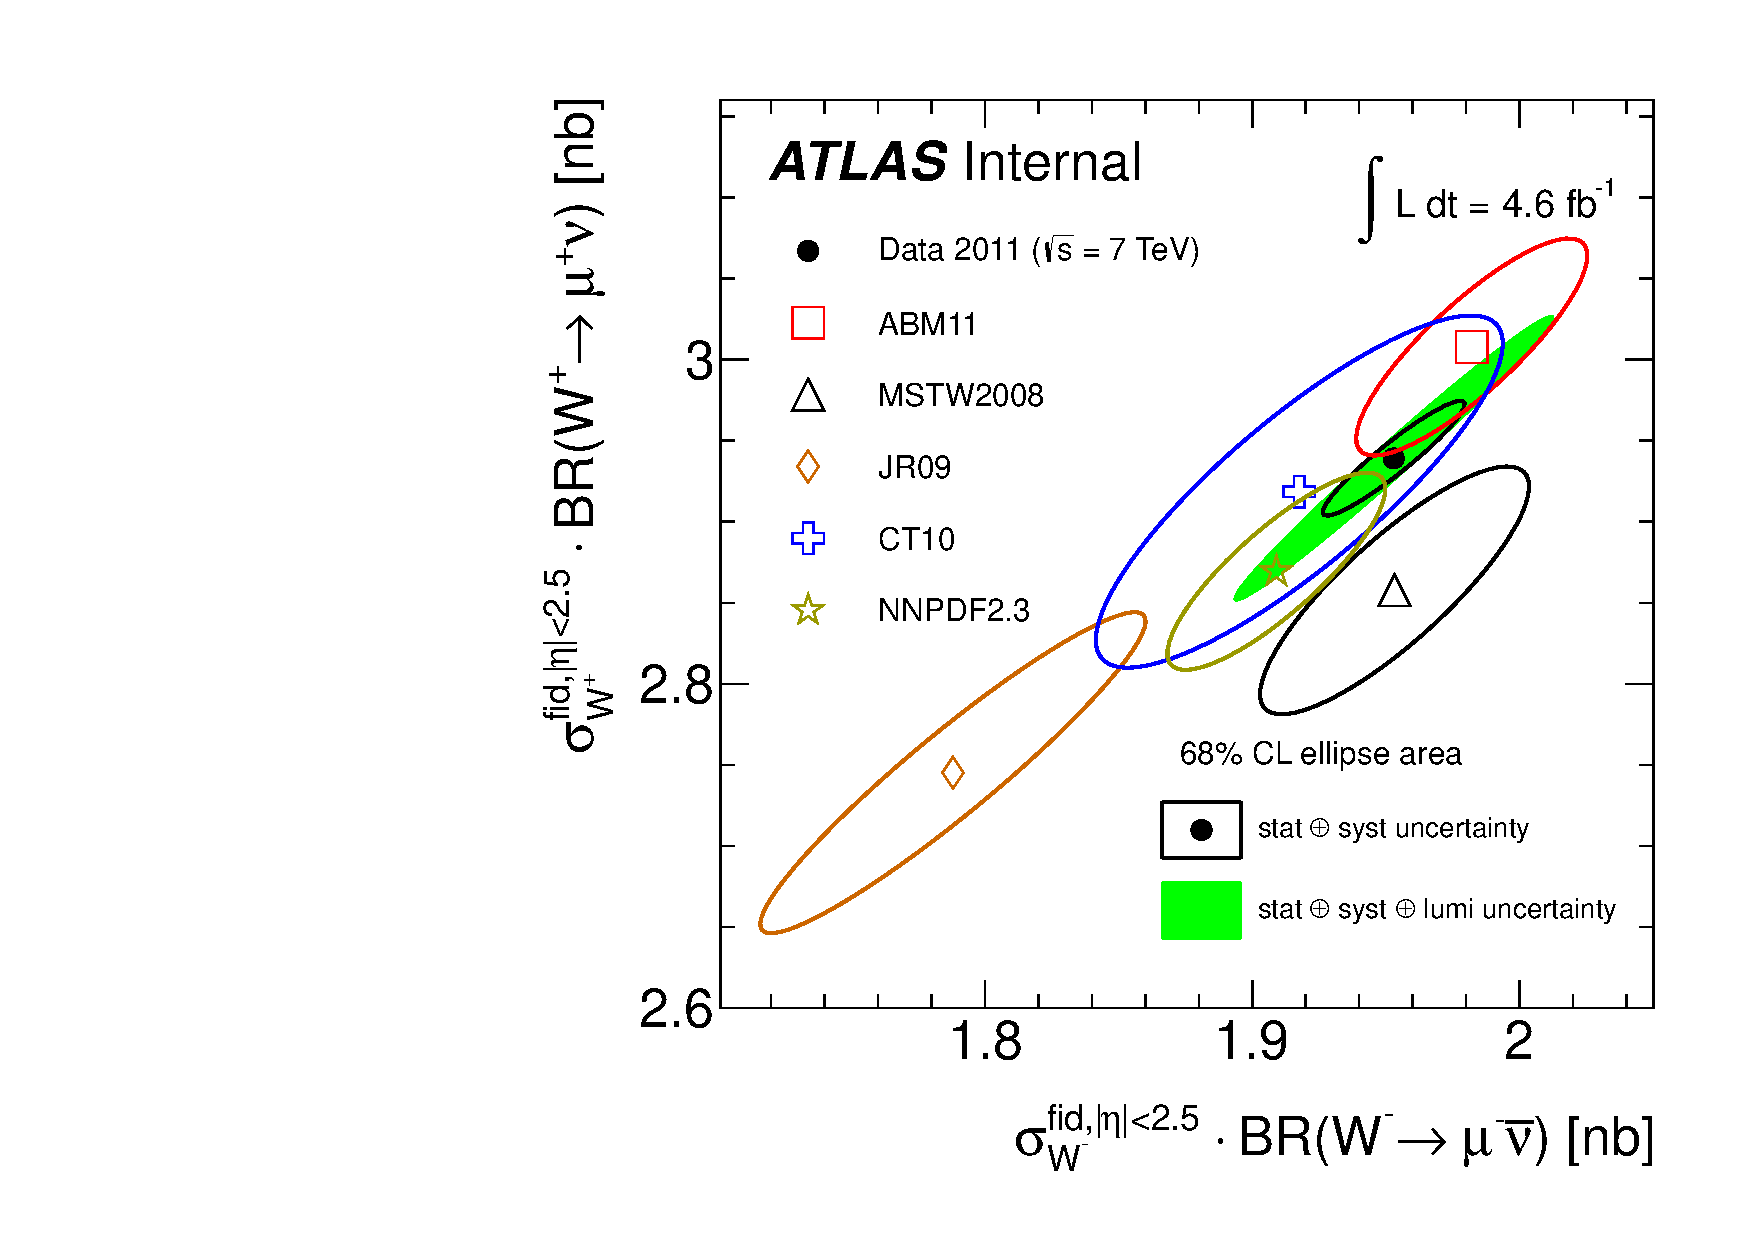
\includegraphics[width=0.6\textwidth]{res/fig/WpWm_ellipse}
        } 
        \subfigure[Cross-section ratios]{%
	  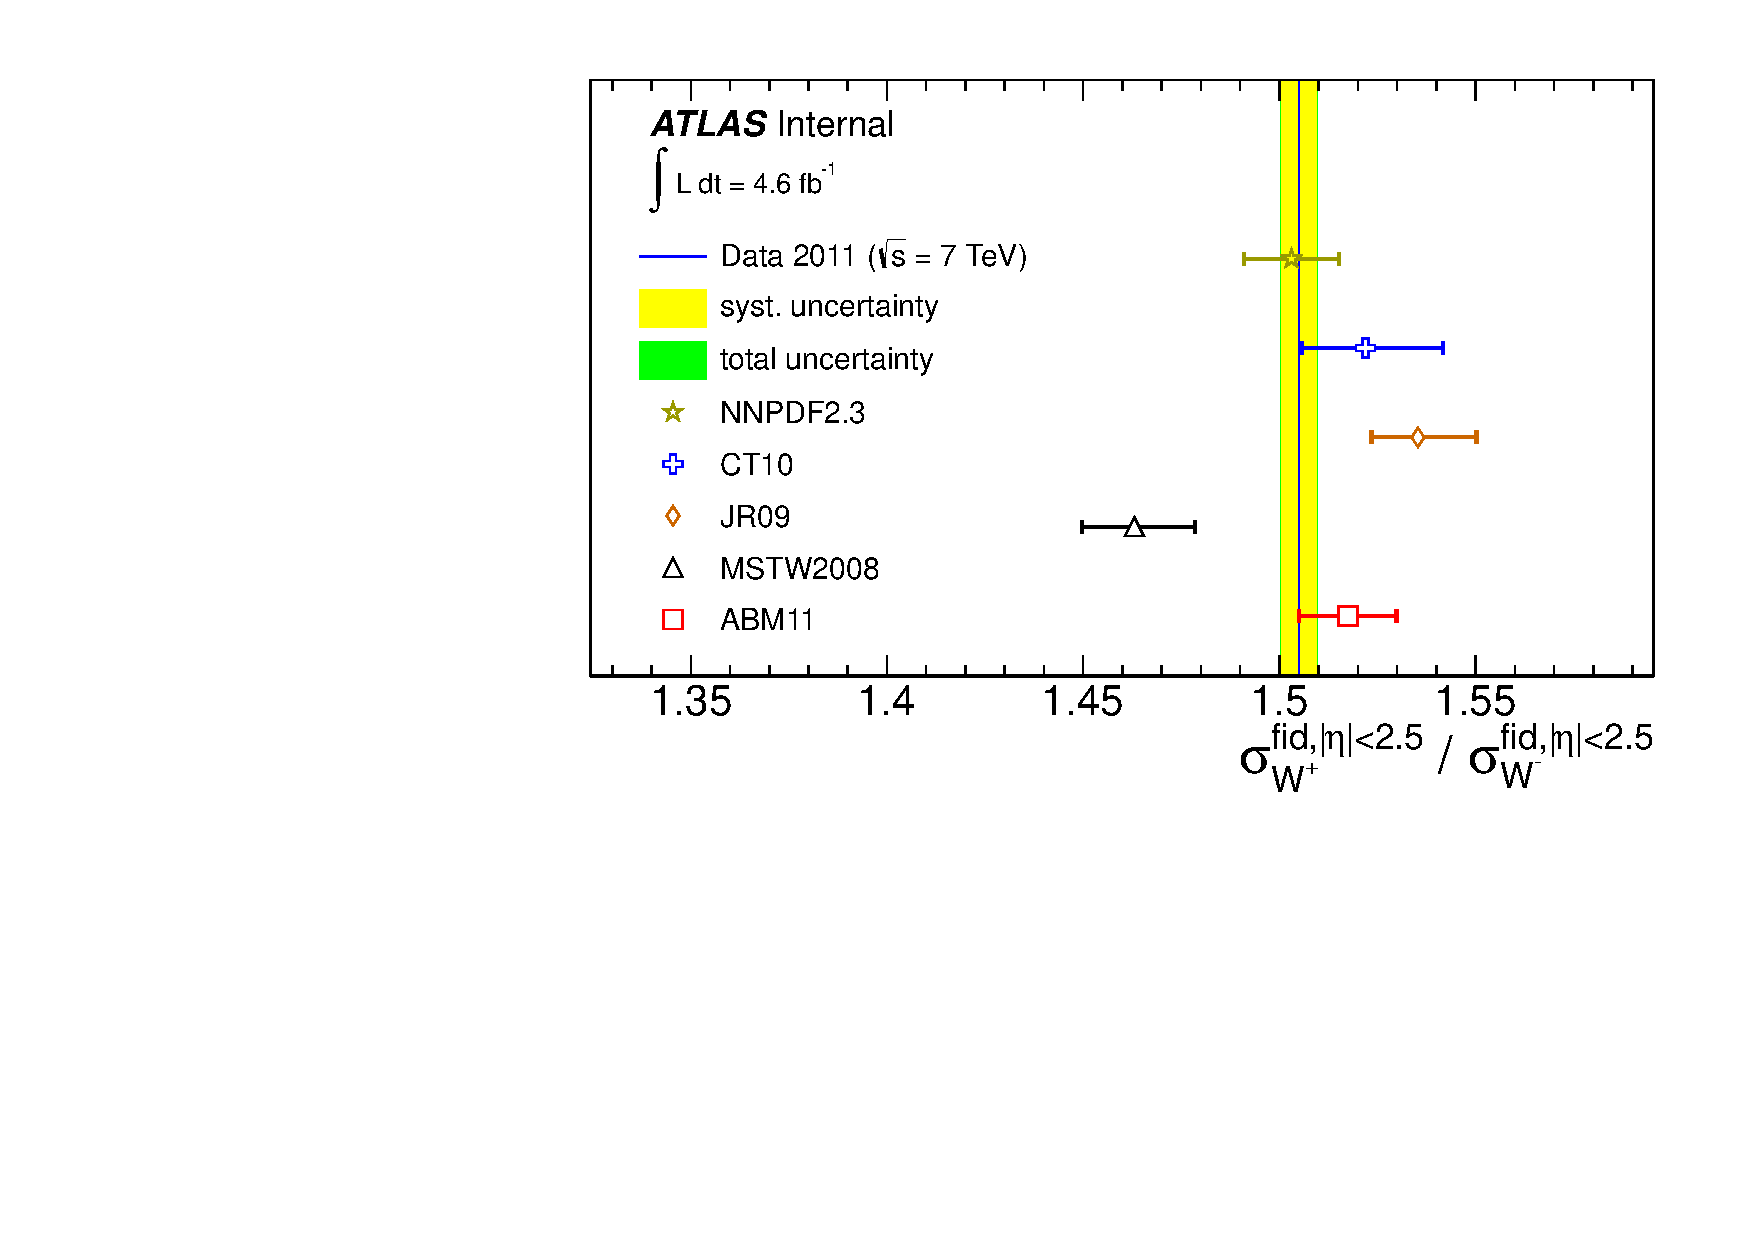
\includegraphics[width=0.6\textwidth]{res/fig/WpWm_ratio}
        }
\caption{ Fiducial cross-sections times leptonic branching ratios of $\sigma_{W^+}$ vs. $\sigma_{W^-}$ (top), and their ratios (bottom).
The data ellipses illustrate the 68\% CL coverage for the total uncertainties (full green) and excluding the luminosity uncertainty (open black).
Theoretical predictions based on various PDF sets are shown with open symbol of different colors.
}
\label{Fig:IntFidCrossSections}
 \end{center}
\end{figure}

%% \begin{figure}
%% \begin{center}
%% 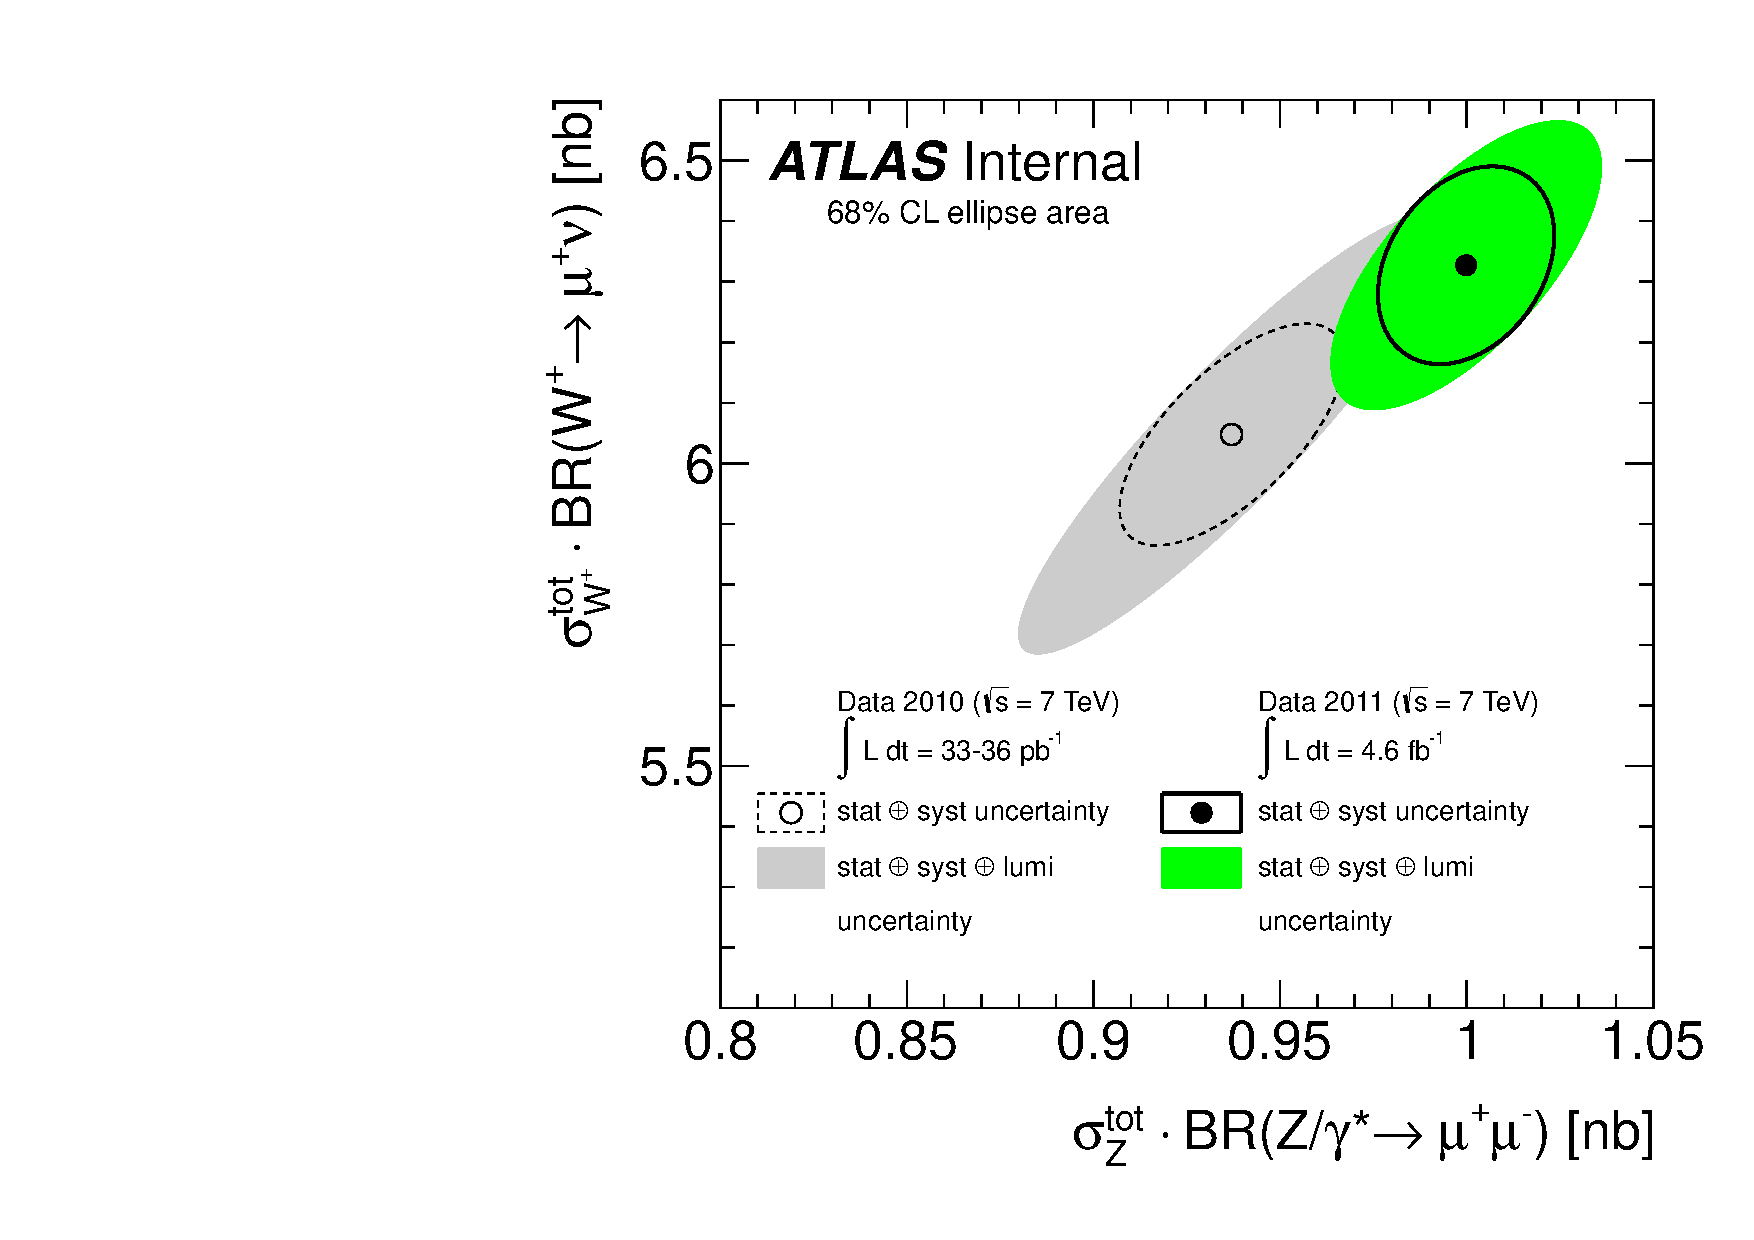
\includegraphics[width=0.47\textwidth]{res/fig/WpZtot_ellipse}\put(-40,100){\Large{\textbf{(a)}}}%
%% 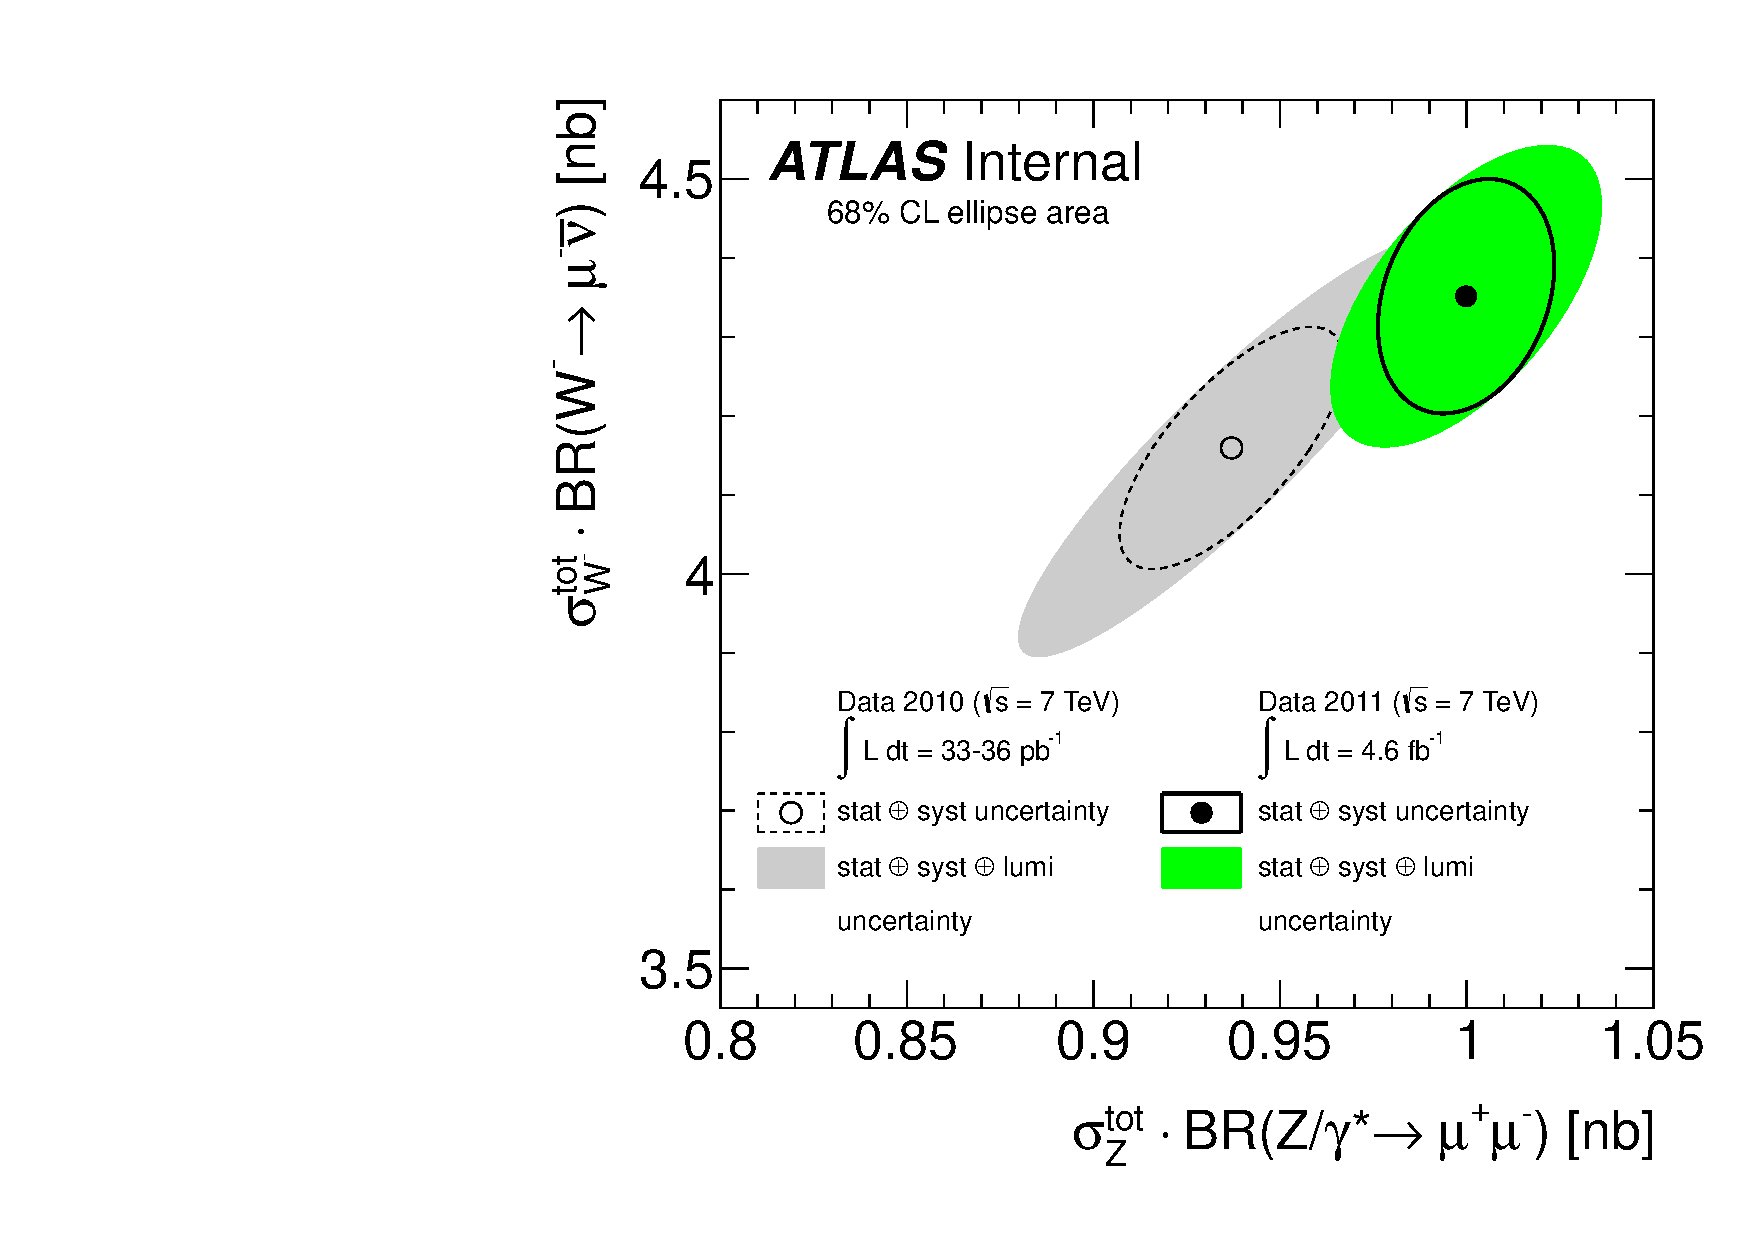
\includegraphics[width=0.47\textwidth]{res/fig/WmZtot_ellipse}\put(-40,100){\Large{\textbf{(b)}}}\\
%% 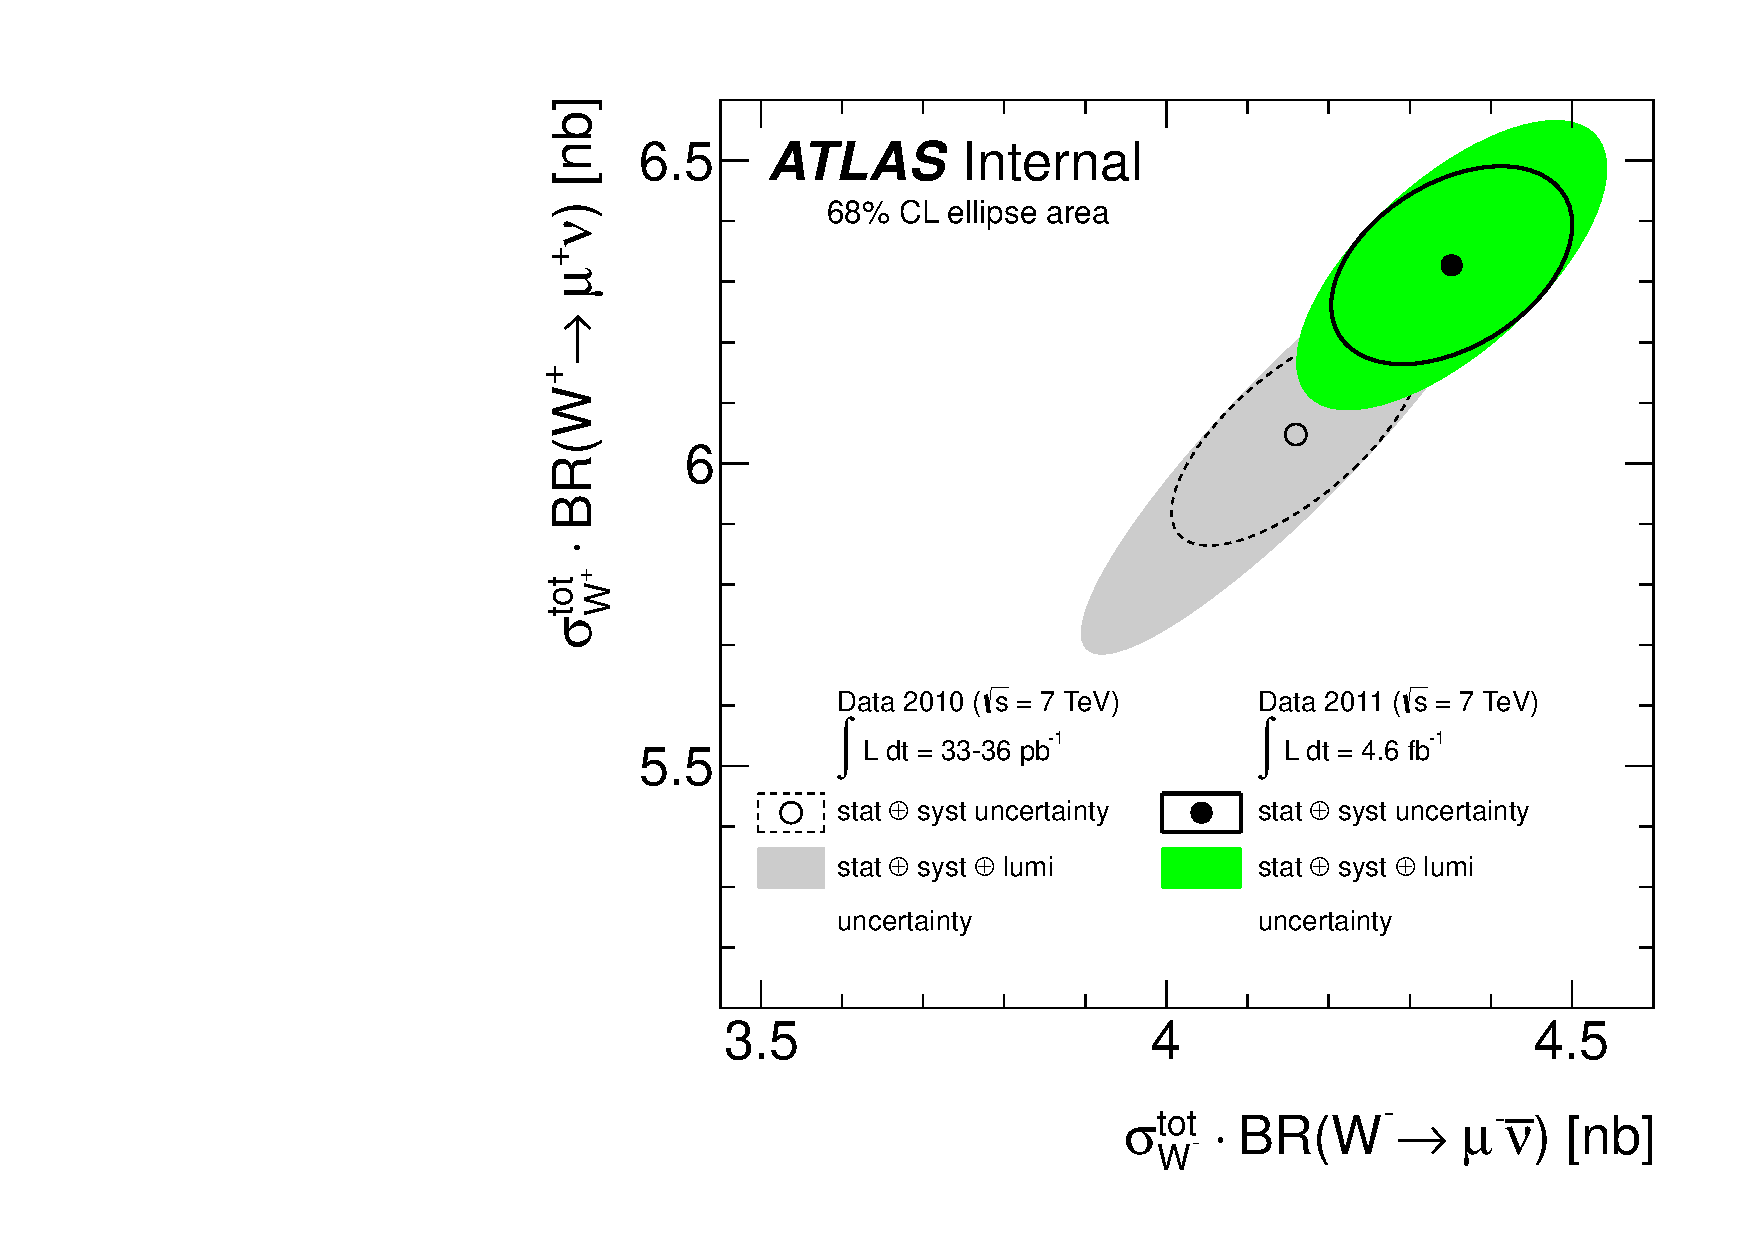
\includegraphics[width=0.47\textwidth]{res/fig/WpWmtot_ellipse}\put(-40,100){\Large{\textbf{(c)}}}%
%% 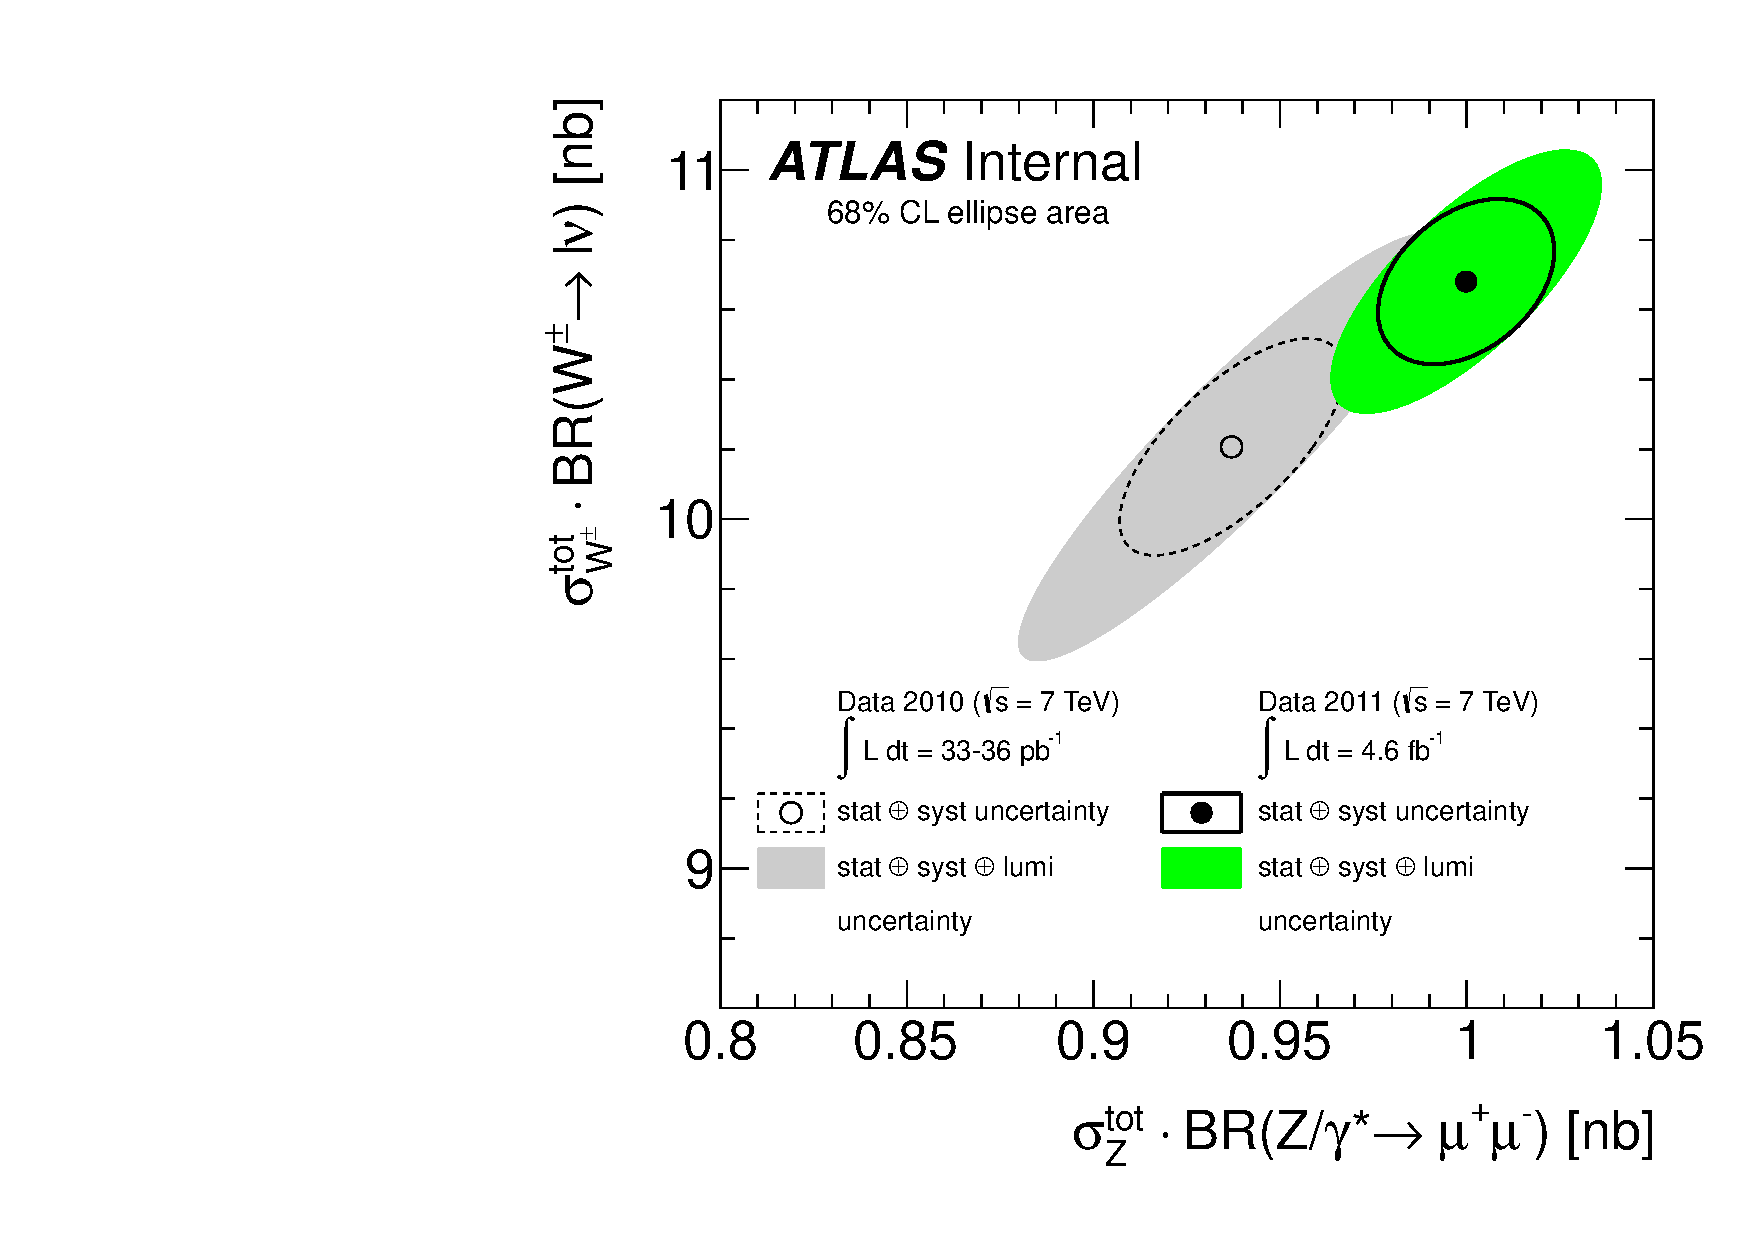
\includegraphics[width=0.47\textwidth]{res/fig/WZtot_ellipse}\put(-40,100){\Large{\textbf{(d)}}}
%% \end{center}
%% \caption{Total cross sections times leptonic branching ratios of $\sigma_{W^+}$ vs. $\sigma_{Z/\gamma^{*}}$ (a),
%% $\sigma_{W^-}$ vs. $\sigma_{Z/\gamma^{*}}$ (b), $\sigma_{W^+}$ vs. $\sigma_{W^-}$ (c) and $\sigma_{W}$ vs. $\sigma_{Z/\gamma^{*}}$ (d).
%% The earlier measurement \protect{\cite{Aad:2011dm}} (open circle) is compared to the new data (filled circle). The ellipses illustrate the 68\% CL coverage for the total uncertainties (filled ellipses) and excluding the luminosity uncertainty (open ellipses).}
%% \label{Fig:IntTotCrossSections}
%% \end{figure}

\subsection{ Single-differential Measurement }
% v21 mu-only

Fig.~\ref{fig:Comb:NNLO:W} shows single-differential $W^{\pm}$ cross-section as a function of $|\eta|$ and compares them with theoretical predictions using different PDF sets. For $W^-$, ABM11 and HERAPDF1.5 provide the best description of the data; MSTW2008 and CT10 are slightly worse but stay within their respective uncertainty envelopes; NNPDF2.3 undershoots the data in the central region, and JR09 fails everywhere but the most forward bins. For $W^+$, HERAPDF1.5 and CT10 provide the best description of the data; ABM11 slightly overshoots the data at forward $\eta$, while NNPDF2.3, MSTW2008 and especially JR09 undershoot across the entire $\eta$ range.

\begin{figure}[phtb]
  \begin{center}
          \subfigure[$d\sigma/d|\eta_{\mu^{-}}|$]{%
         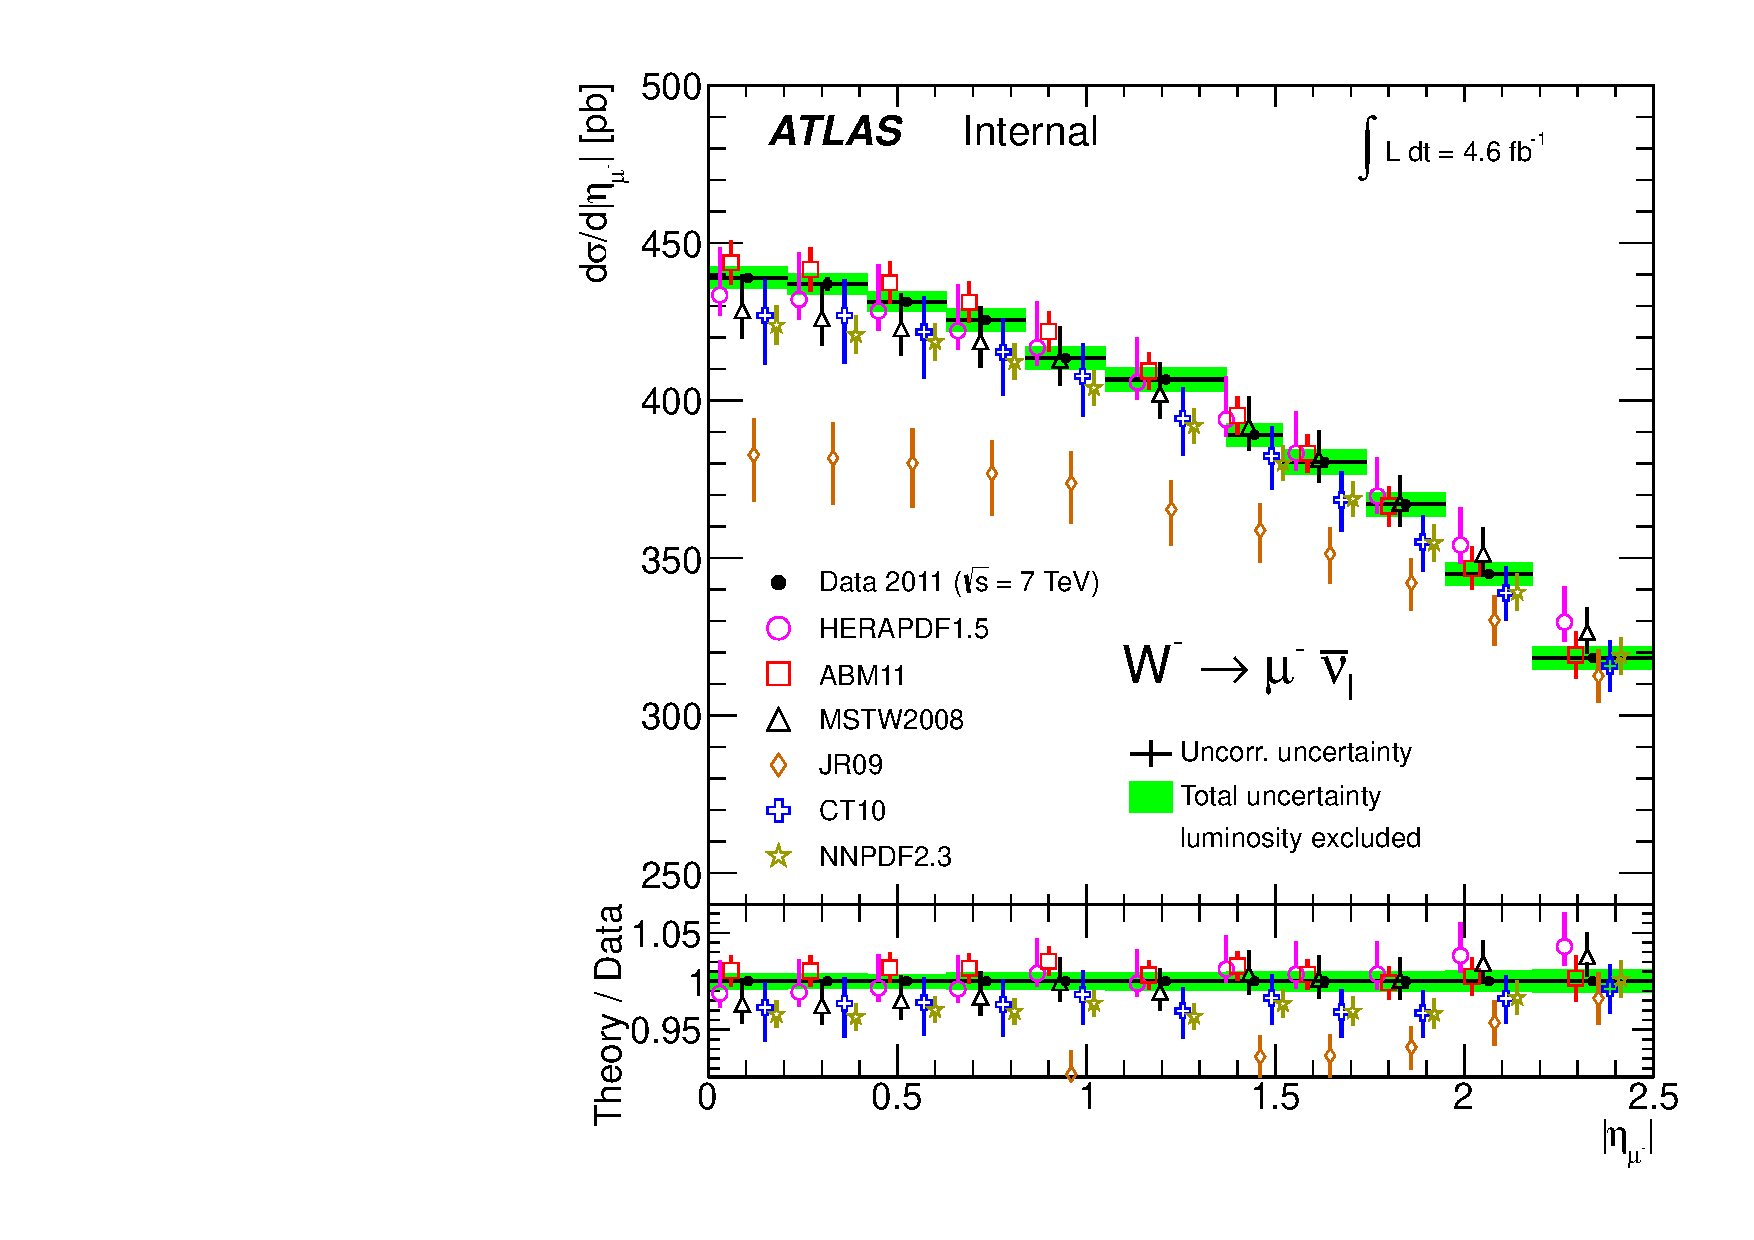
\includegraphics[width=0.60\textwidth]{res/fig/WMeta25_NNLO_combined}
        }               
        \subfigure[$d\sigma/d|\eta_{\mu^{+}}|$]{%
          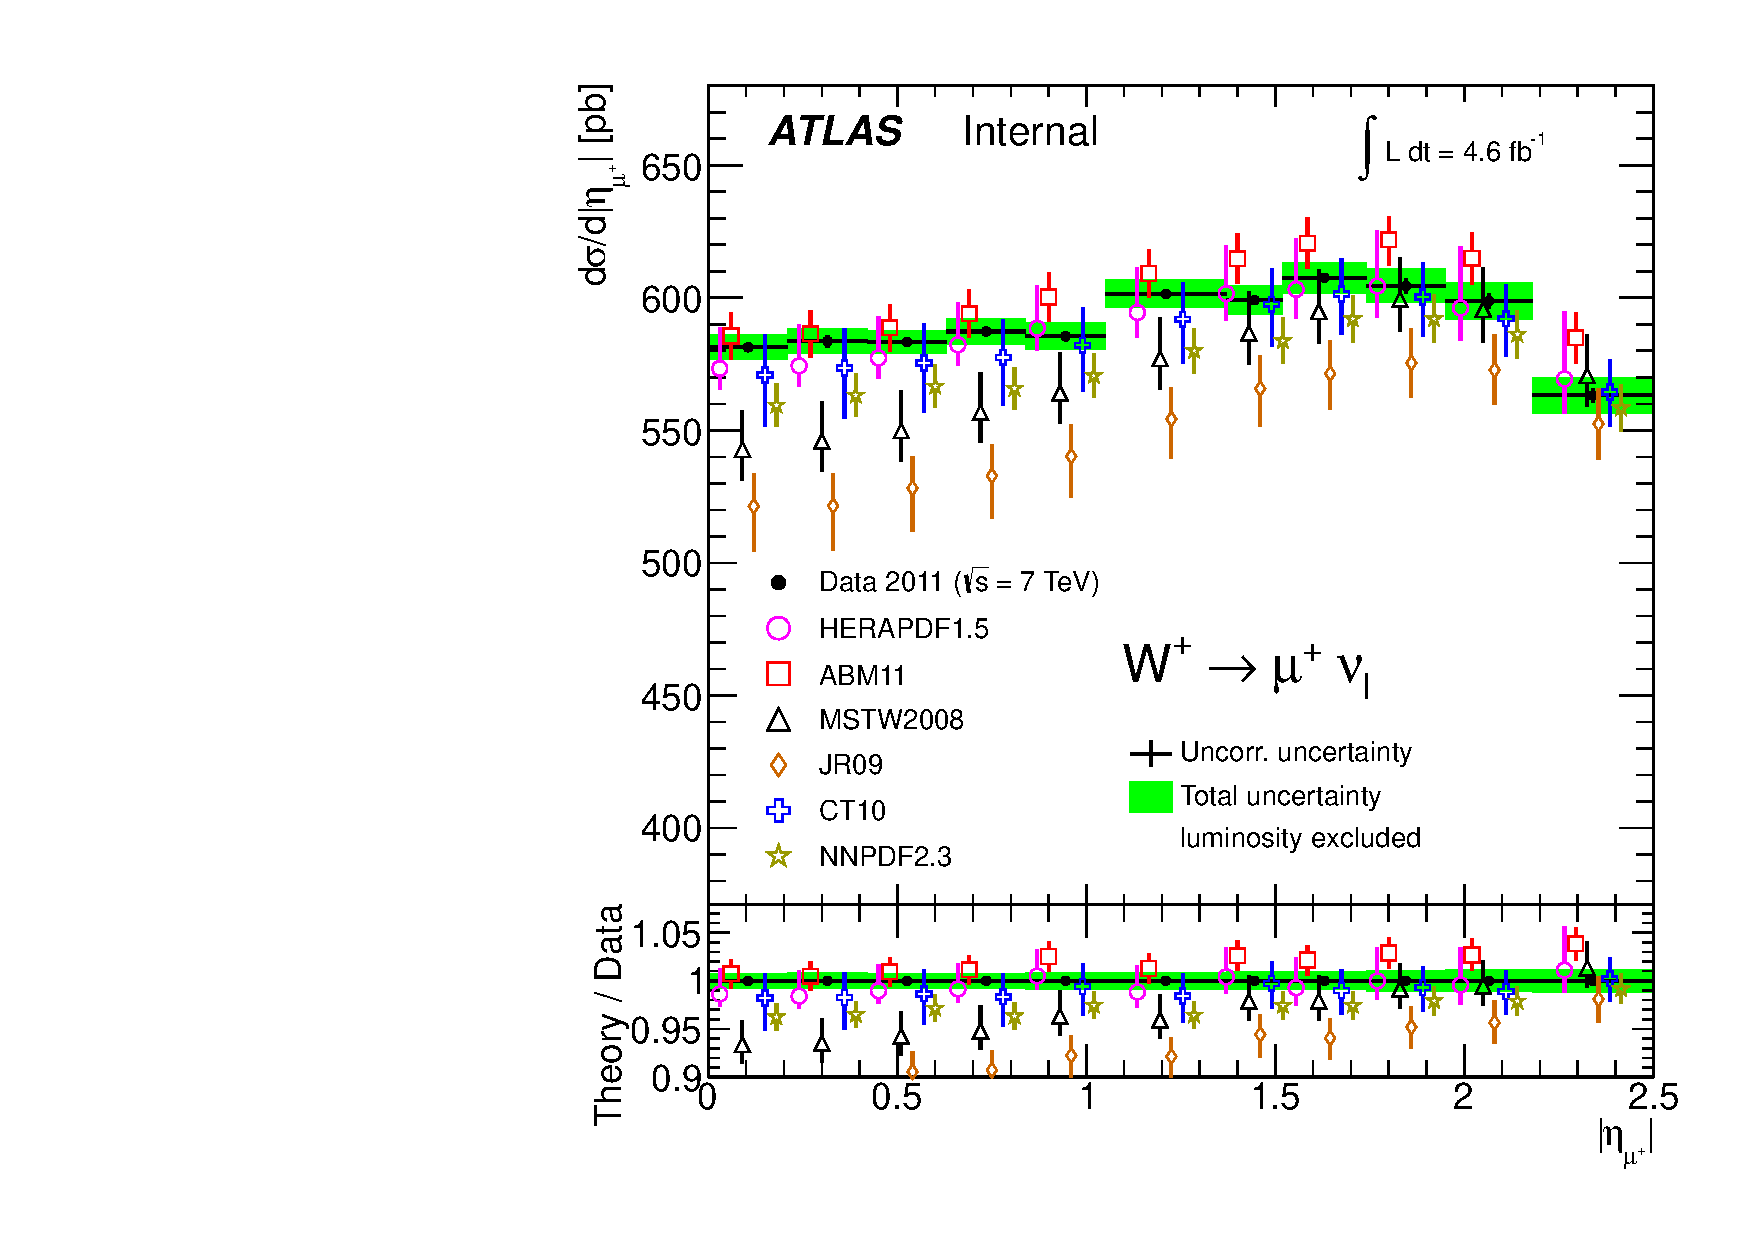
\includegraphics[width=0.60\textwidth]{res/fig/WPeta25_NNLO_combined}
        }
 \caption{ The single-differential cross-section measurement for \Wpmmn. NNLO QCD predictions using various PDF sets (open symbols) are compared to the data (full points). The predictions are displaced within each bin for clarity. }
\label{fig:Comb:NNLO:W}
 \end{center}
\end{figure}

\subsection{ W Charge Asymmetry }
% v21 mu-only

W charge asymmetry is derived from single-differential cross-sections and aims to reduce those systematics that are highly correlated between $W^+$ and $W^-$. Formally, the asymmetry is defined as:
 
$$A_{\mu} = \frac{d\sigma_{W^{+}}/d|\eta_{\mu^{+}}| - d\sigma_{W^{-}}/d|\eta_{\mu^{-}}|}{d\sigma_{W^{+}}/d|\eta_{\mu^{+}}| + d\sigma_{W^{-}}/d|\eta_{\mu^{-}}|}$$

Fig.~\ref{fig:Comb:NNLO:Wasym25} shows $A_{\mu}$ as a function of $|\eta|$ for different PDF sets. NNPDF2.3 provides the best description of the data, followed by HERAPDF1.5 and CT10. JR09 overshoots the data at central $\eta$, while ABM11 overshoots in the forward regions. MSTW2008 fails to adequately describe the asymmetry.

\begin{figure}
\begin{center}
   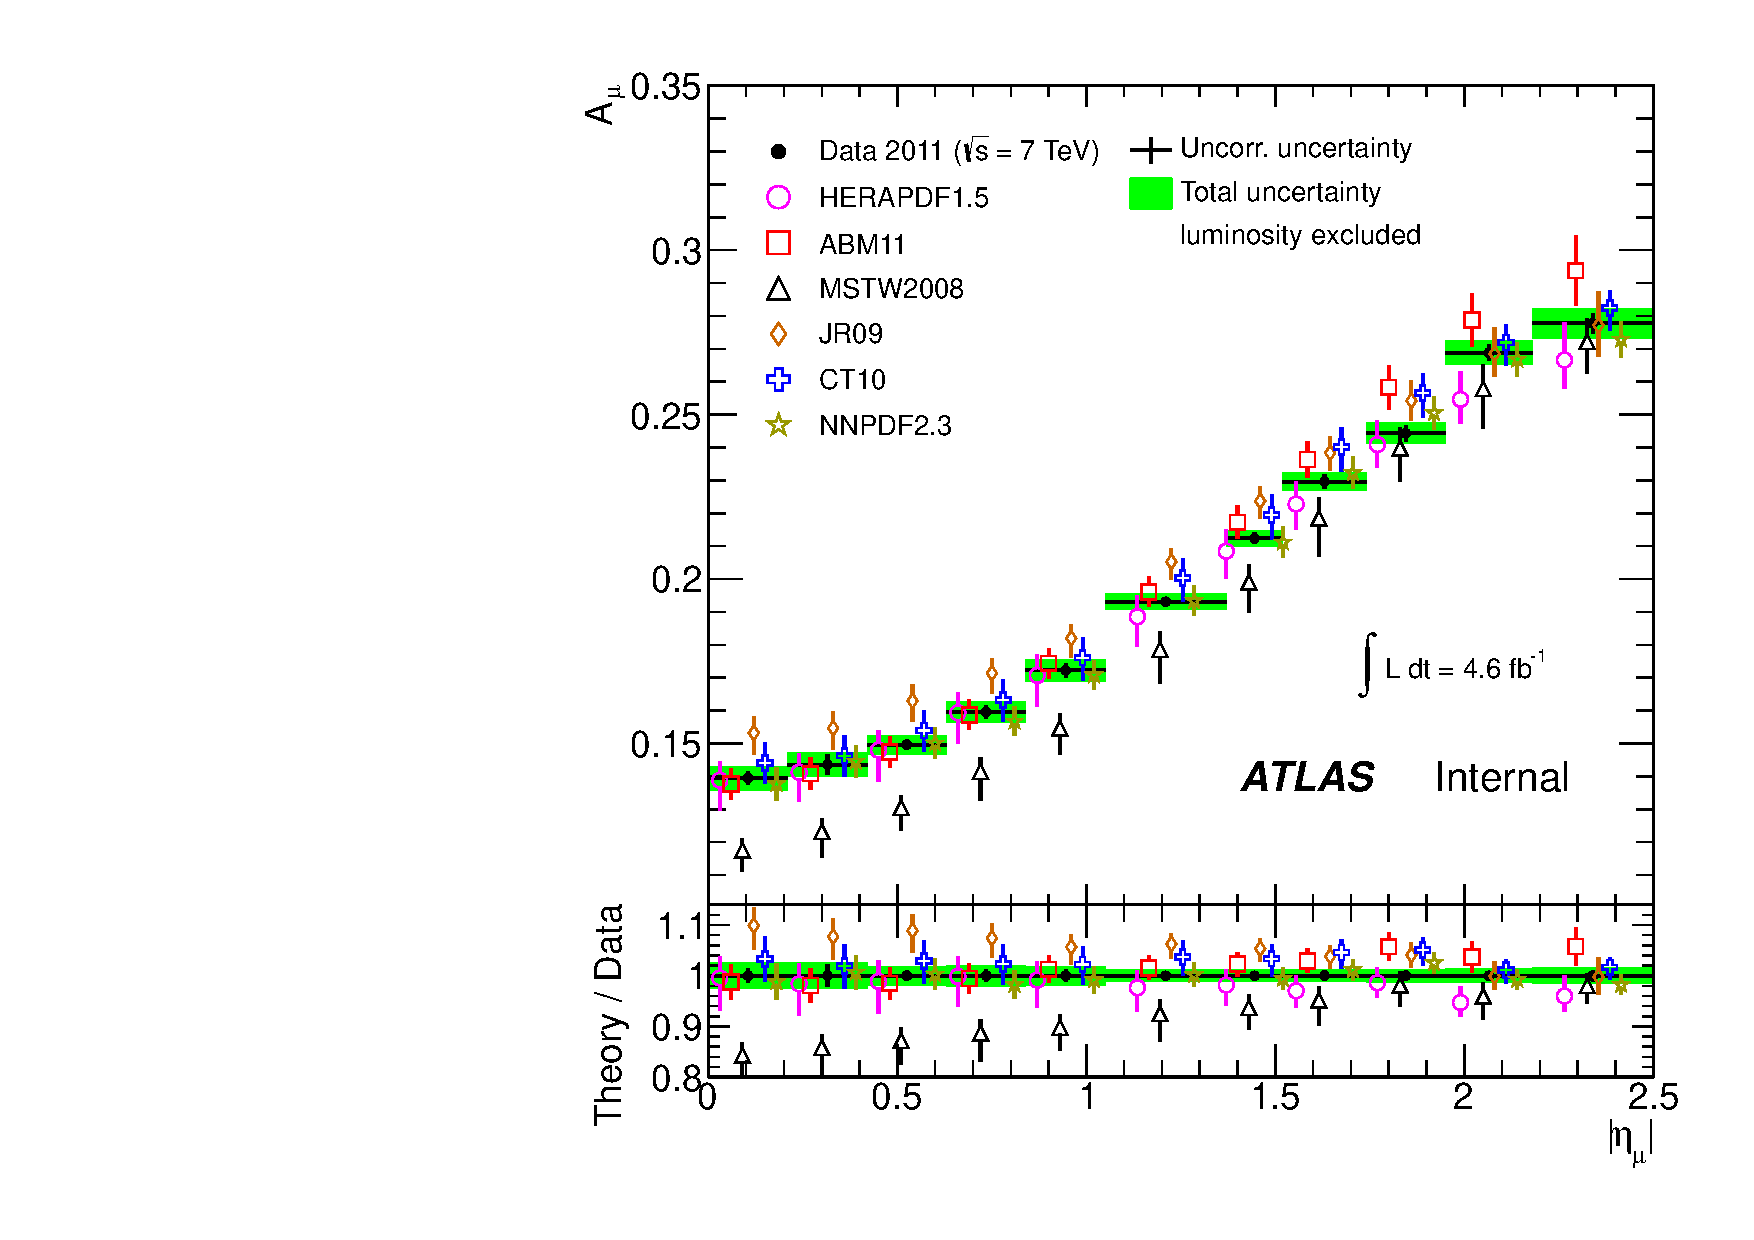
\includegraphics[width=0.75\textwidth]{res/fig/Wasym25_NNLO_combined}
\end{center}
\caption{ Fiducial $W$ charge asymmetry as a function of $|\eta_{\mu}|$.
NNLO QCD predictions using various PDF sets (open symbols) are compared to the data (full points).
The predictions are displaced within each bin for clarity.
}
\label{fig:Comb:NNLO:Wasym25}
\end{figure}

\clearpage
\subsection{ Double-differential Measurement }
% v14 mu+e (waiting for updates)

Figs.~\ref{fig:Comb:NNLO:W2dNEG_1}~-~\ref{fig:Comb:NNLO:W2dPOS_3} show double-differential $W^{\pm}$ cross-sections in slices of muon $p_T$. The data lies between the predictions of various PDF sets for $30<p_T<45$ GeV. However, at lower and higher values of $p_T$, all PDFs tend to undershoot the data. This is consistent with the fact that the existing tunes of DYNNLO program fail to describe boson $p_T$ and polarization accurately. Moreover, the Jacobian $p_T$ is smeared in data due to soft radiation / parton showering, which cannot be described by fixed-order predictions.

\begin{figure}[phtb]
  \begin{center}
        \subfigure[\ptOne]{%
	  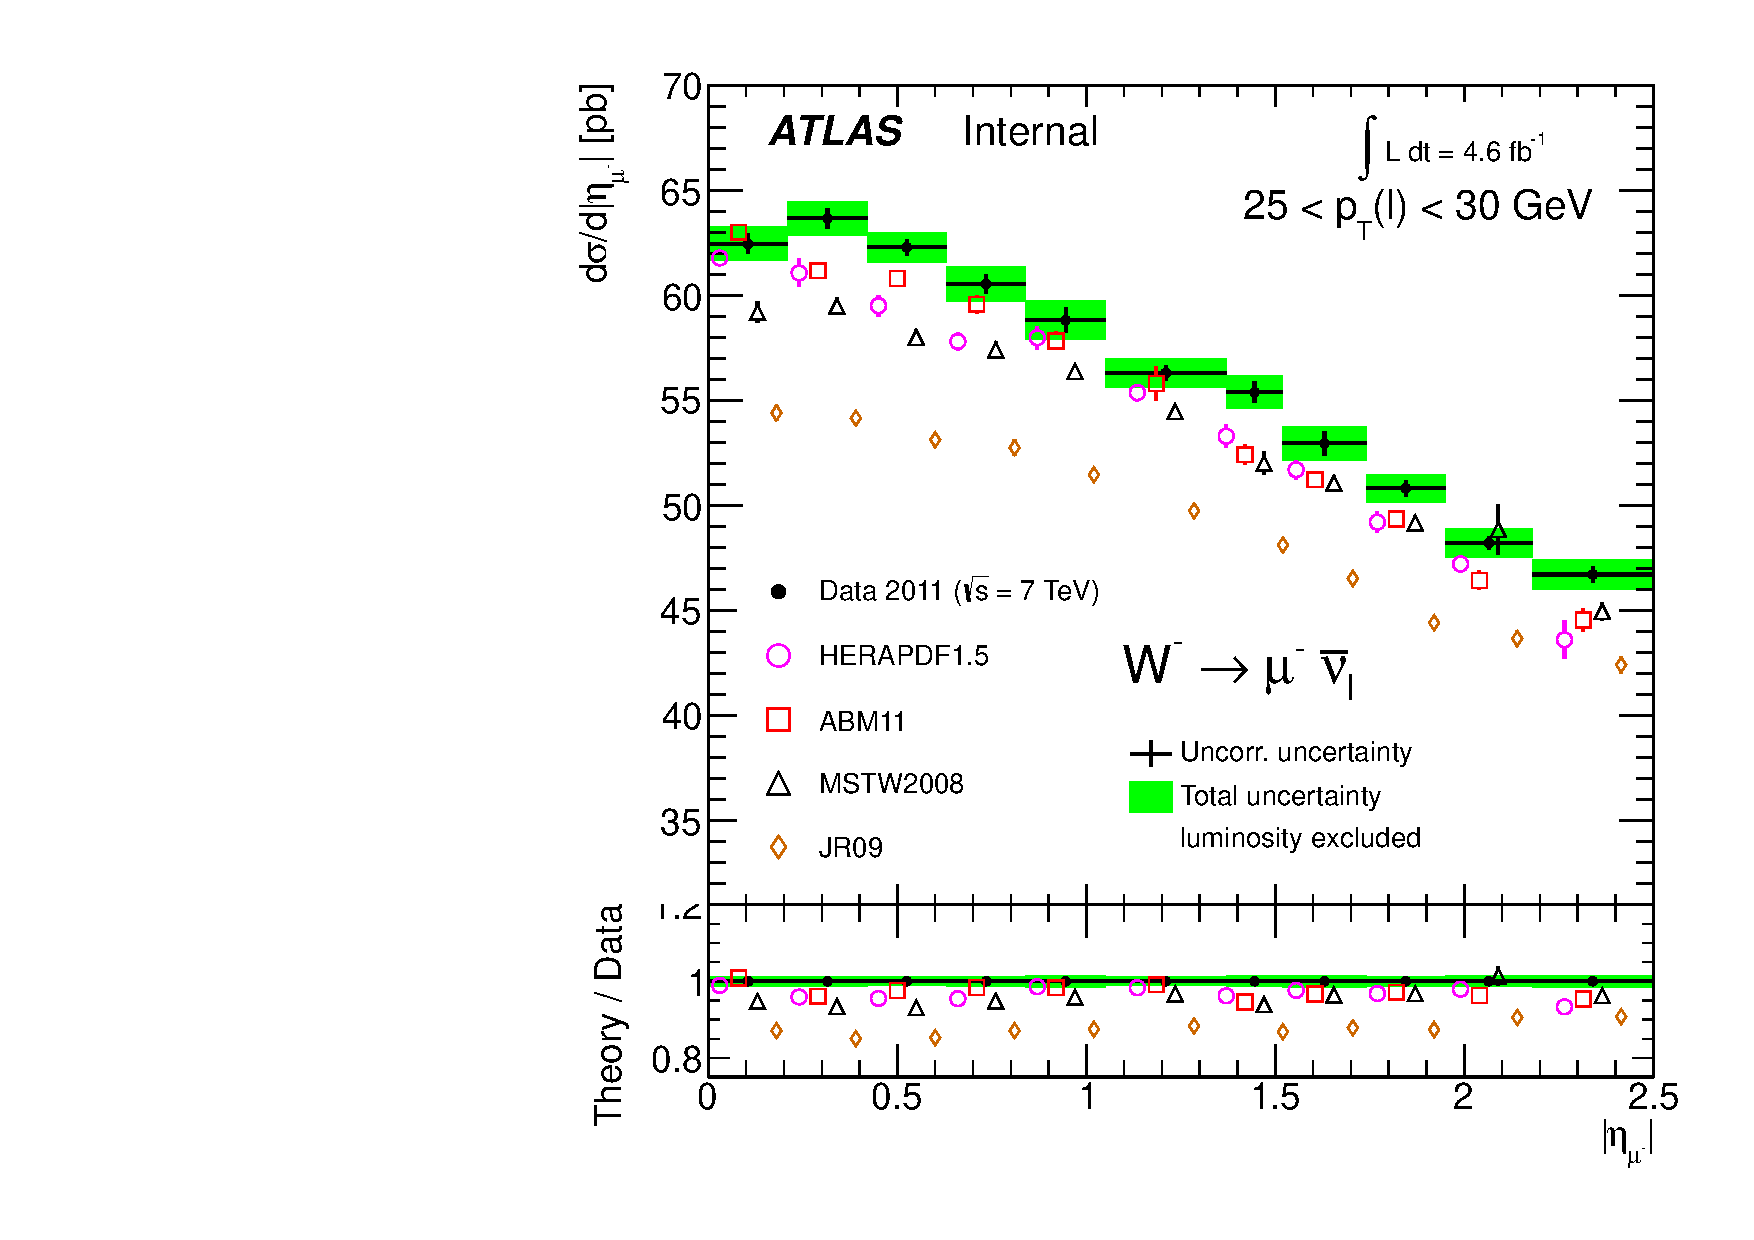
\includegraphics[width=0.55\textwidth]{res/fig/WMetaPt25_30_NNLO_combined}
        }
       \subfigure[\ptTwo]{%
	  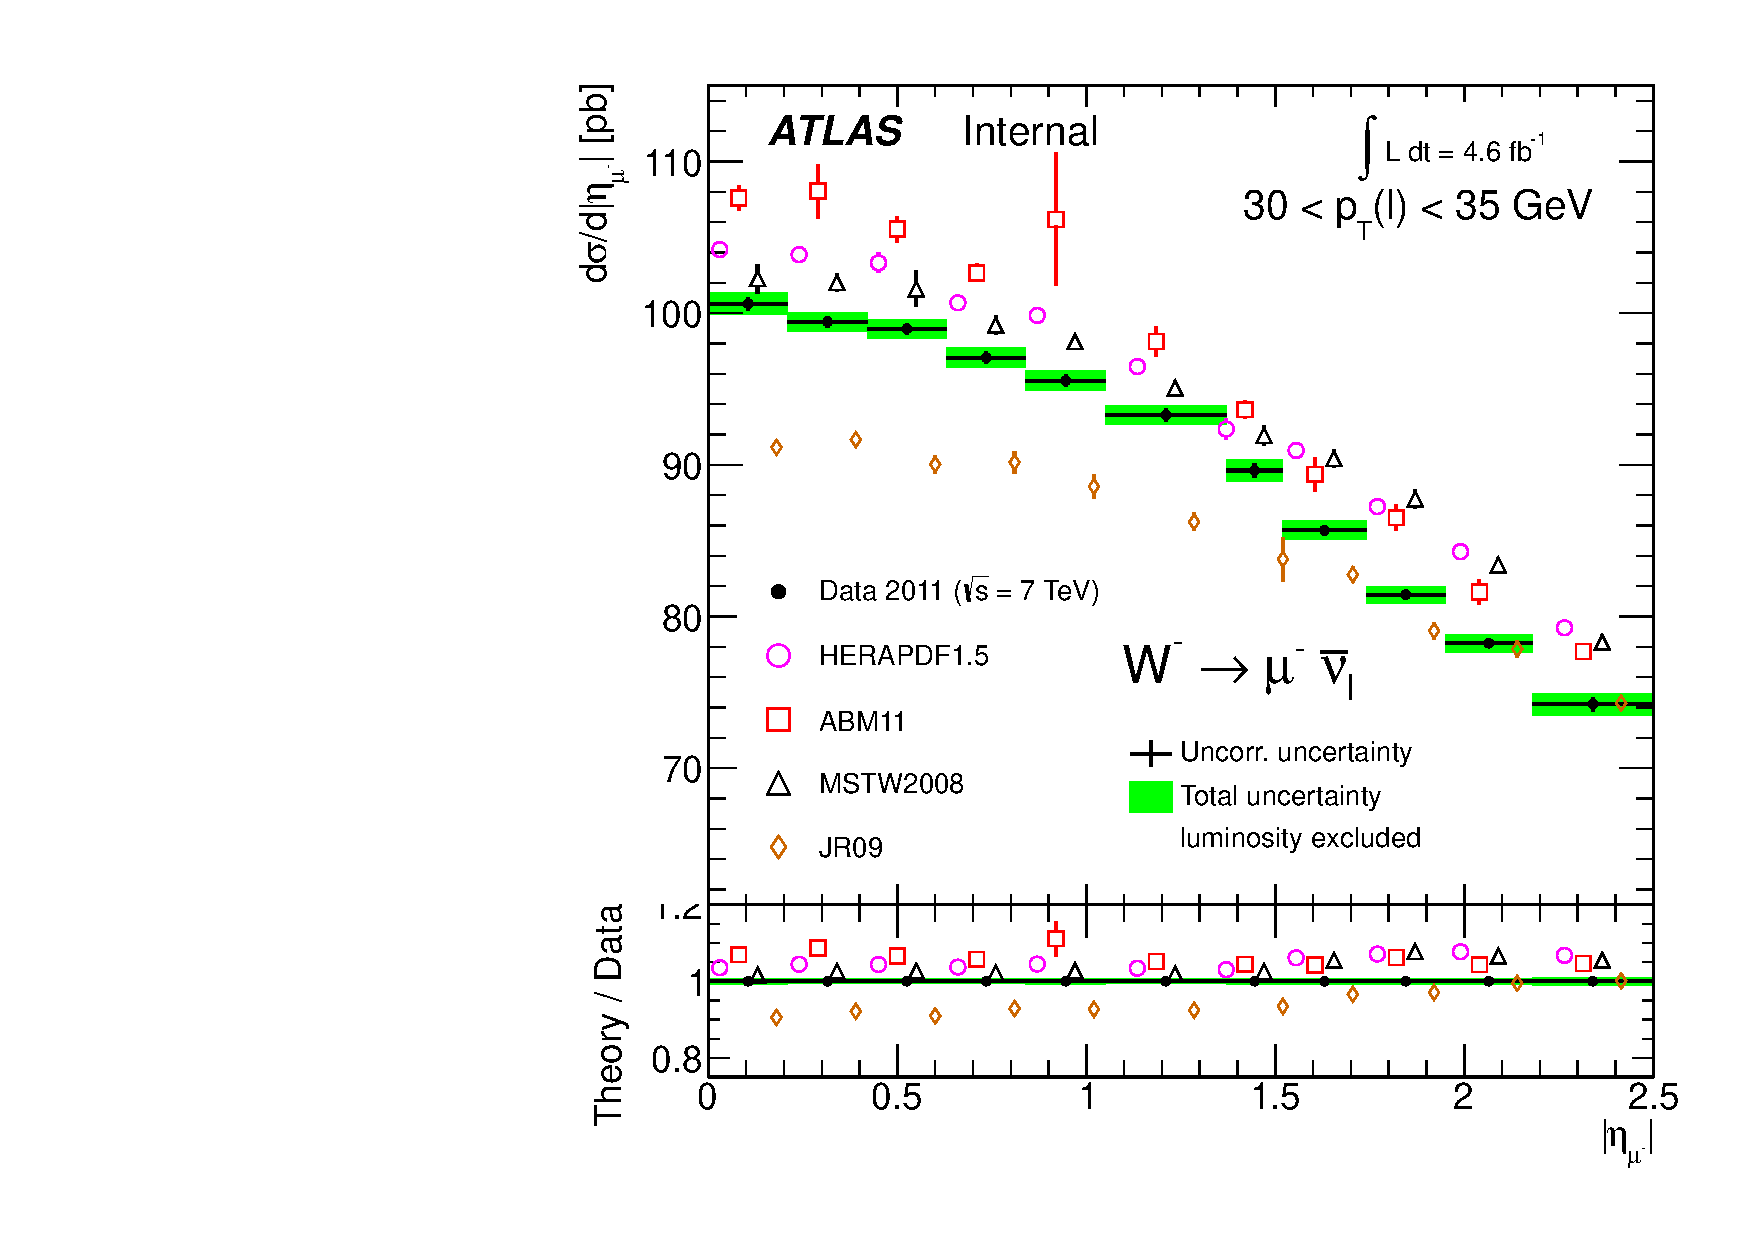
\includegraphics[width=0.55\textwidth]{res/fig/WMetaPt30_35_NNLO_combined}
        }
 \caption{ The double-differential cross-section measurement for \Wminusmunu\ in $p_T$ slices: \ptOne\ and \ptTwo. NNLO QCD predictions using various PDF sets (open symbols) are compared to the data (full points). The predictions are displaced within each bin for clarity. For technical reasons, the uncertainty on predictions excludes the uncertainty from the PDF error envelope. }
 \label{fig:Comb:NNLO:W2dNEG_1}
 \end{center}
\end{figure}

\begin{figure}[phtb]
  \begin{center}
       \subfigure[\ptThree]{%
	  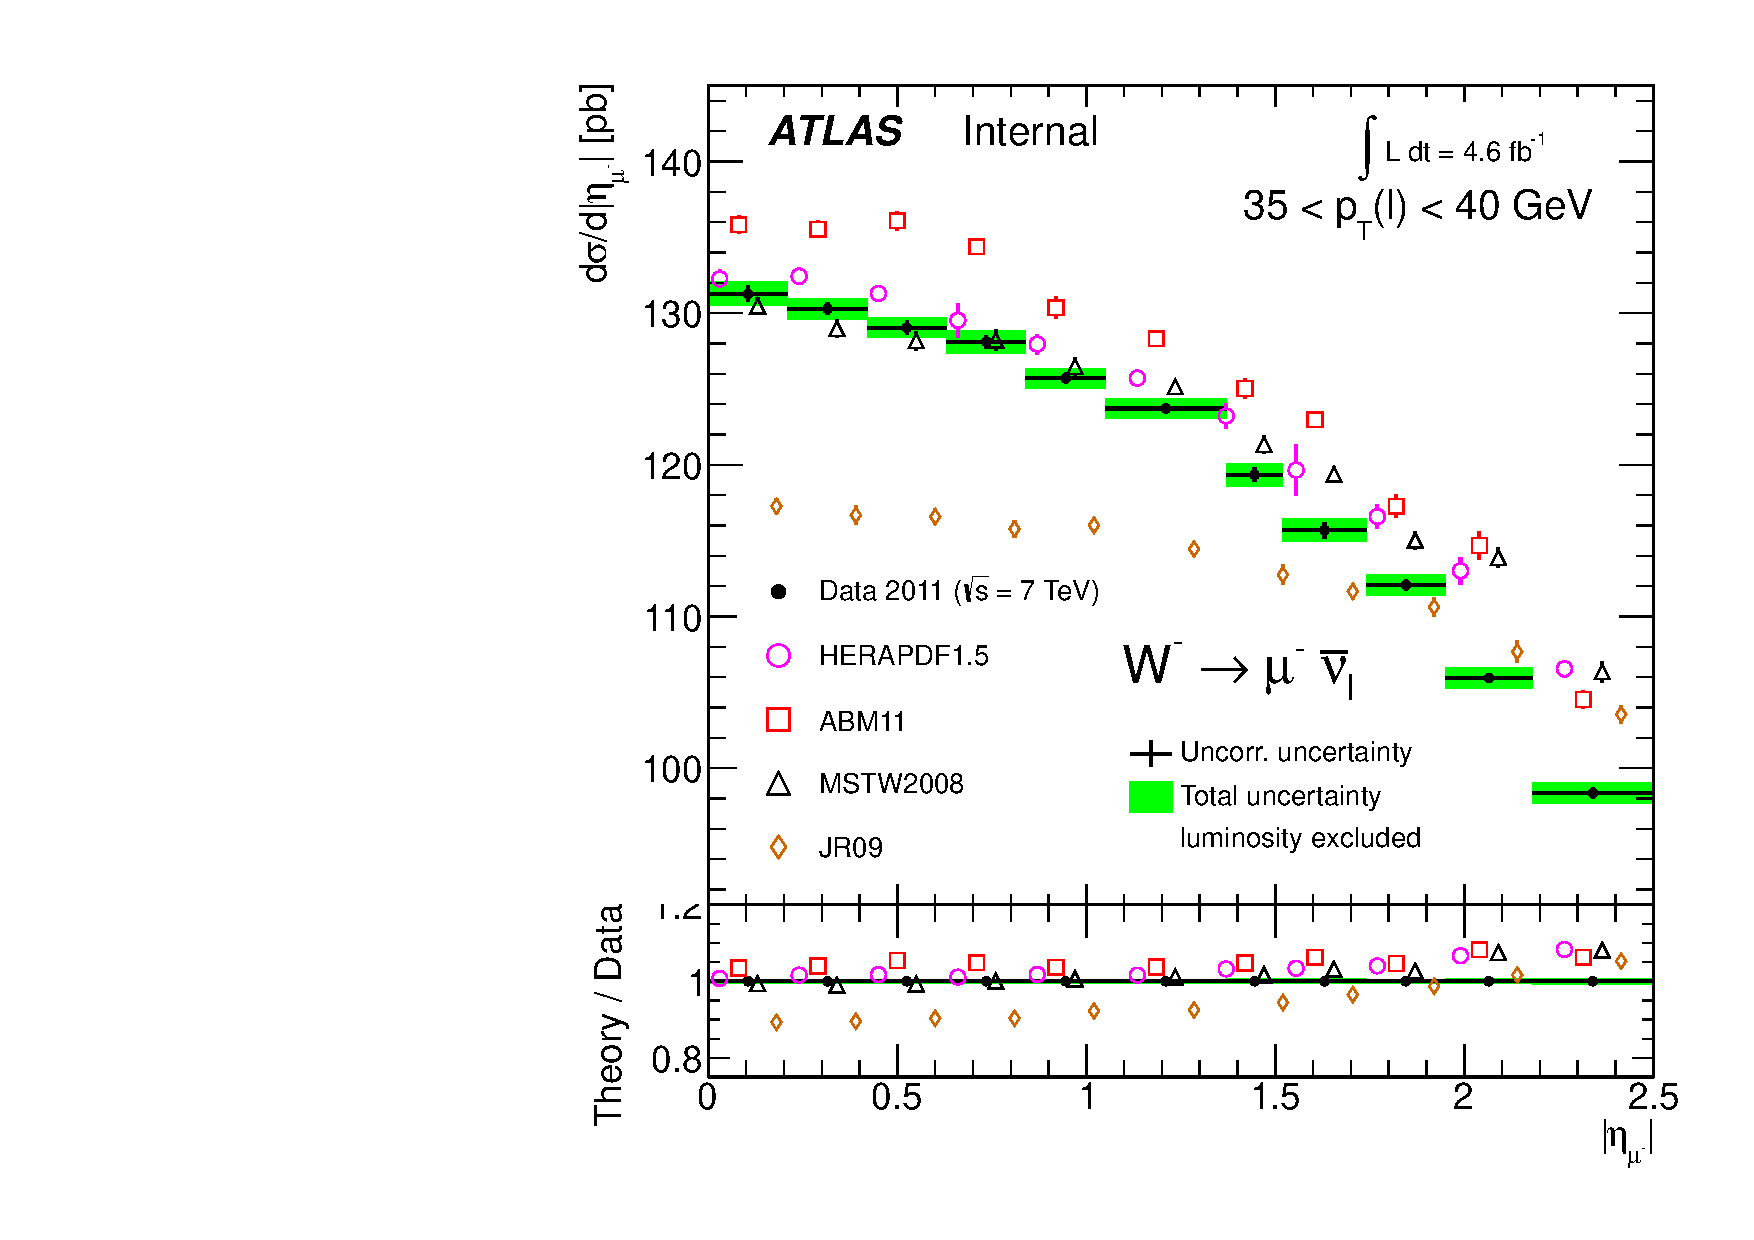
\includegraphics[width=0.55\textwidth]{res/fig/WMetaPt35_40_NNLO_combined}
        }
       \subfigure[\ptFour]{%
	  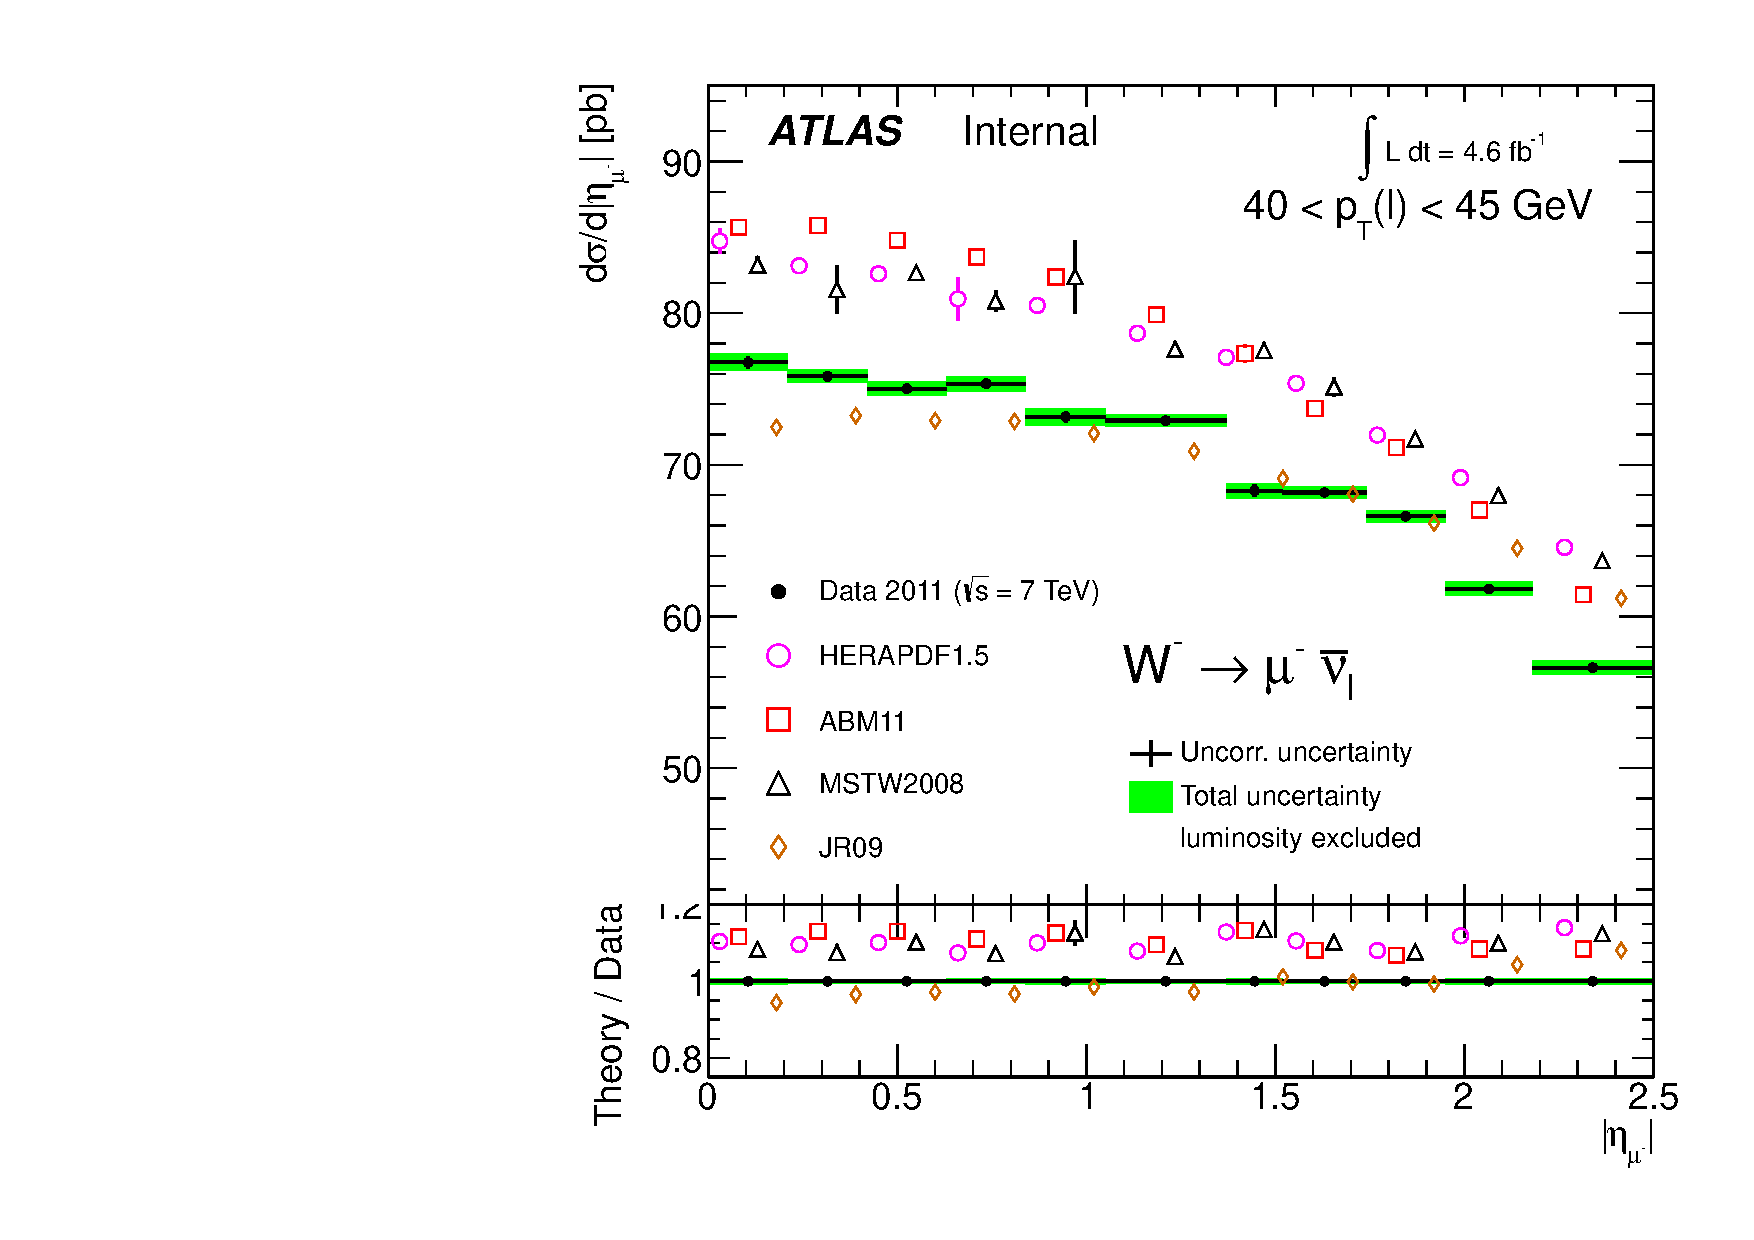
\includegraphics[width=0.55\textwidth]{res/fig/WMetaPt40_45_NNLO_combined}
        }
 \caption{ The double-differential cross-section measurement for \Wminusmunu\ in $p_T$ slices: \ptThree\ and \ptFour. NNLO QCD predictions using various PDF sets (open symbols) are compared to the data (full points). The predictions are displaced within each bin for clarity. For technical reasons, the uncertainty on predictions excludes the uncertainty from the PDF error envelope. }
 \label{fig:Comb:NNLO:W2dNEG_2}
 \end{center}
\end{figure}

\begin{figure}[phtb]
  \begin{center}
       \subfigure[\ptFive]{%
	  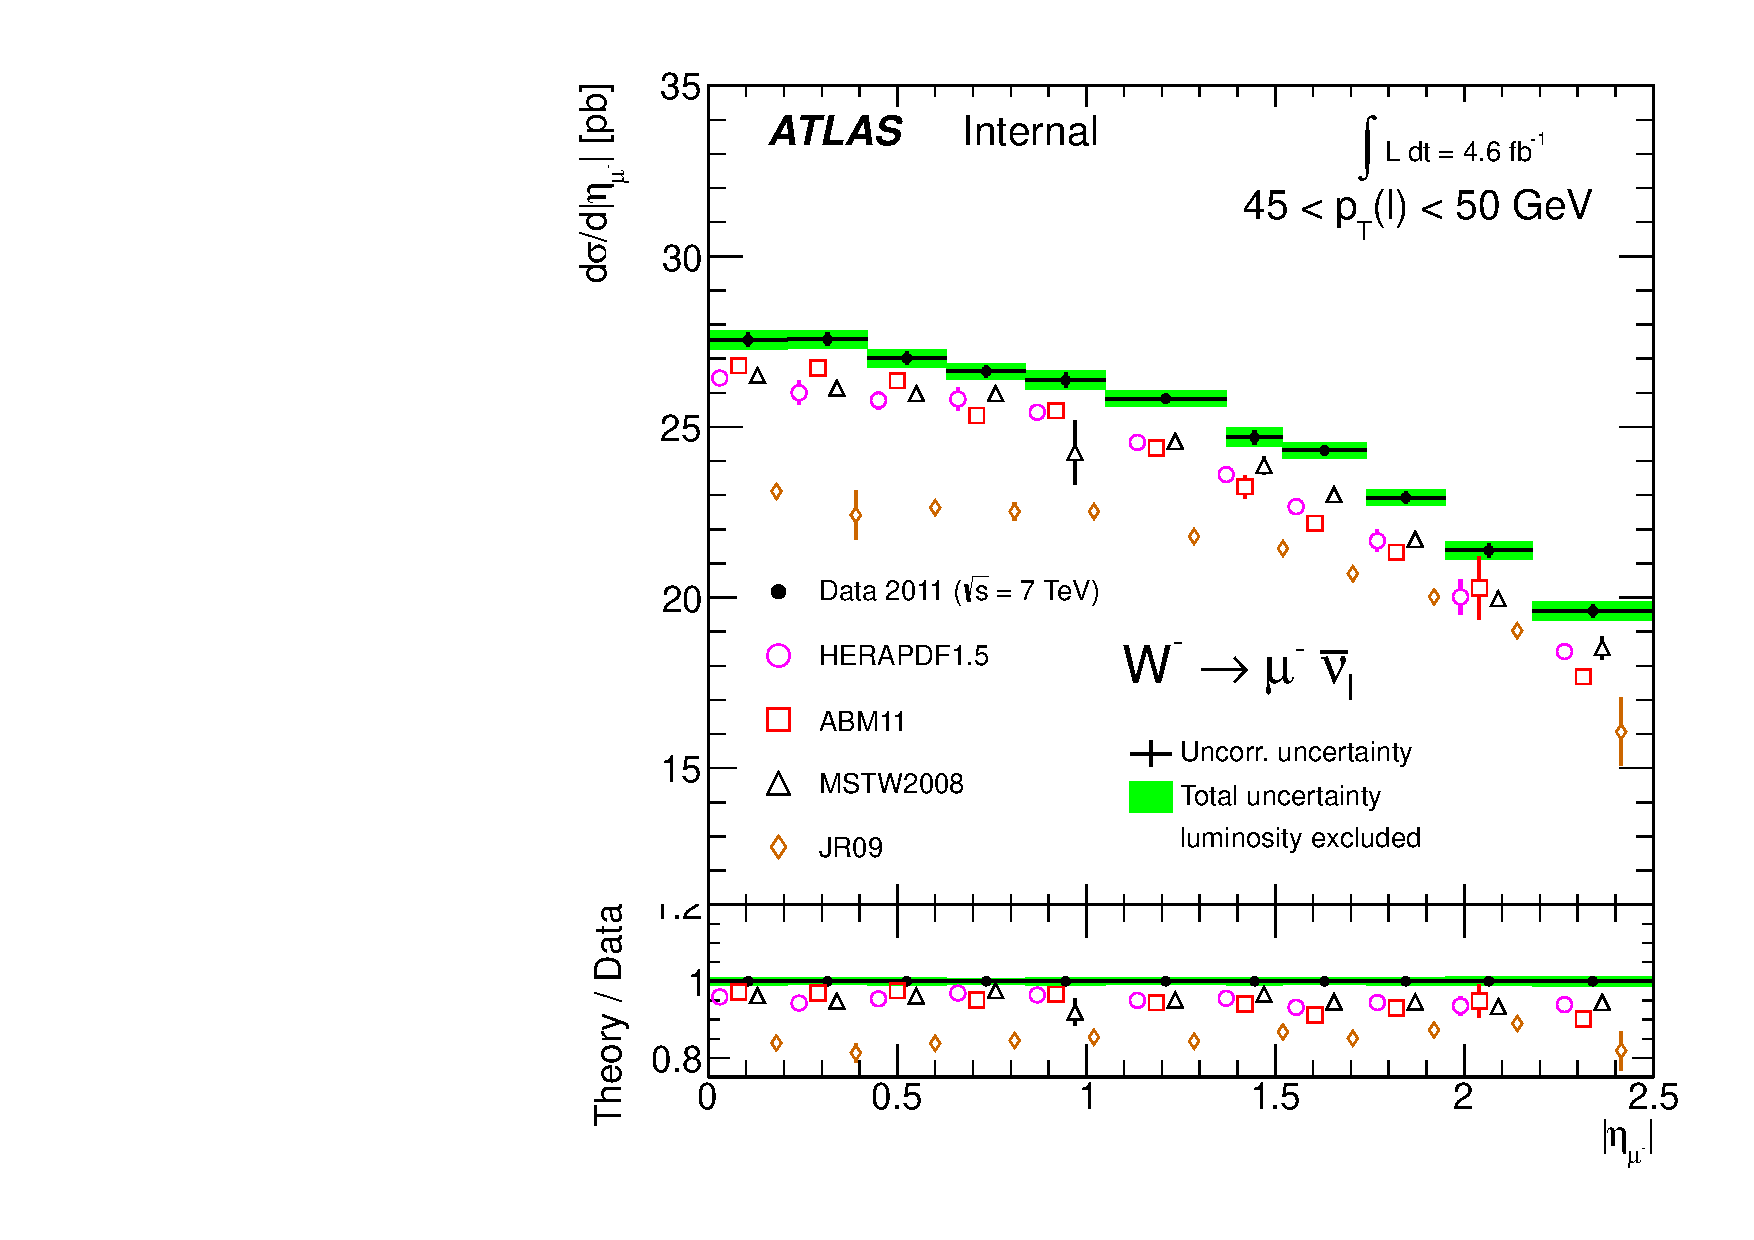
\includegraphics[width=0.55\textwidth]{res/fig/WMetaPt45_50_NNLO_combined}
        }
       \subfigure[\ptSix]{%
	  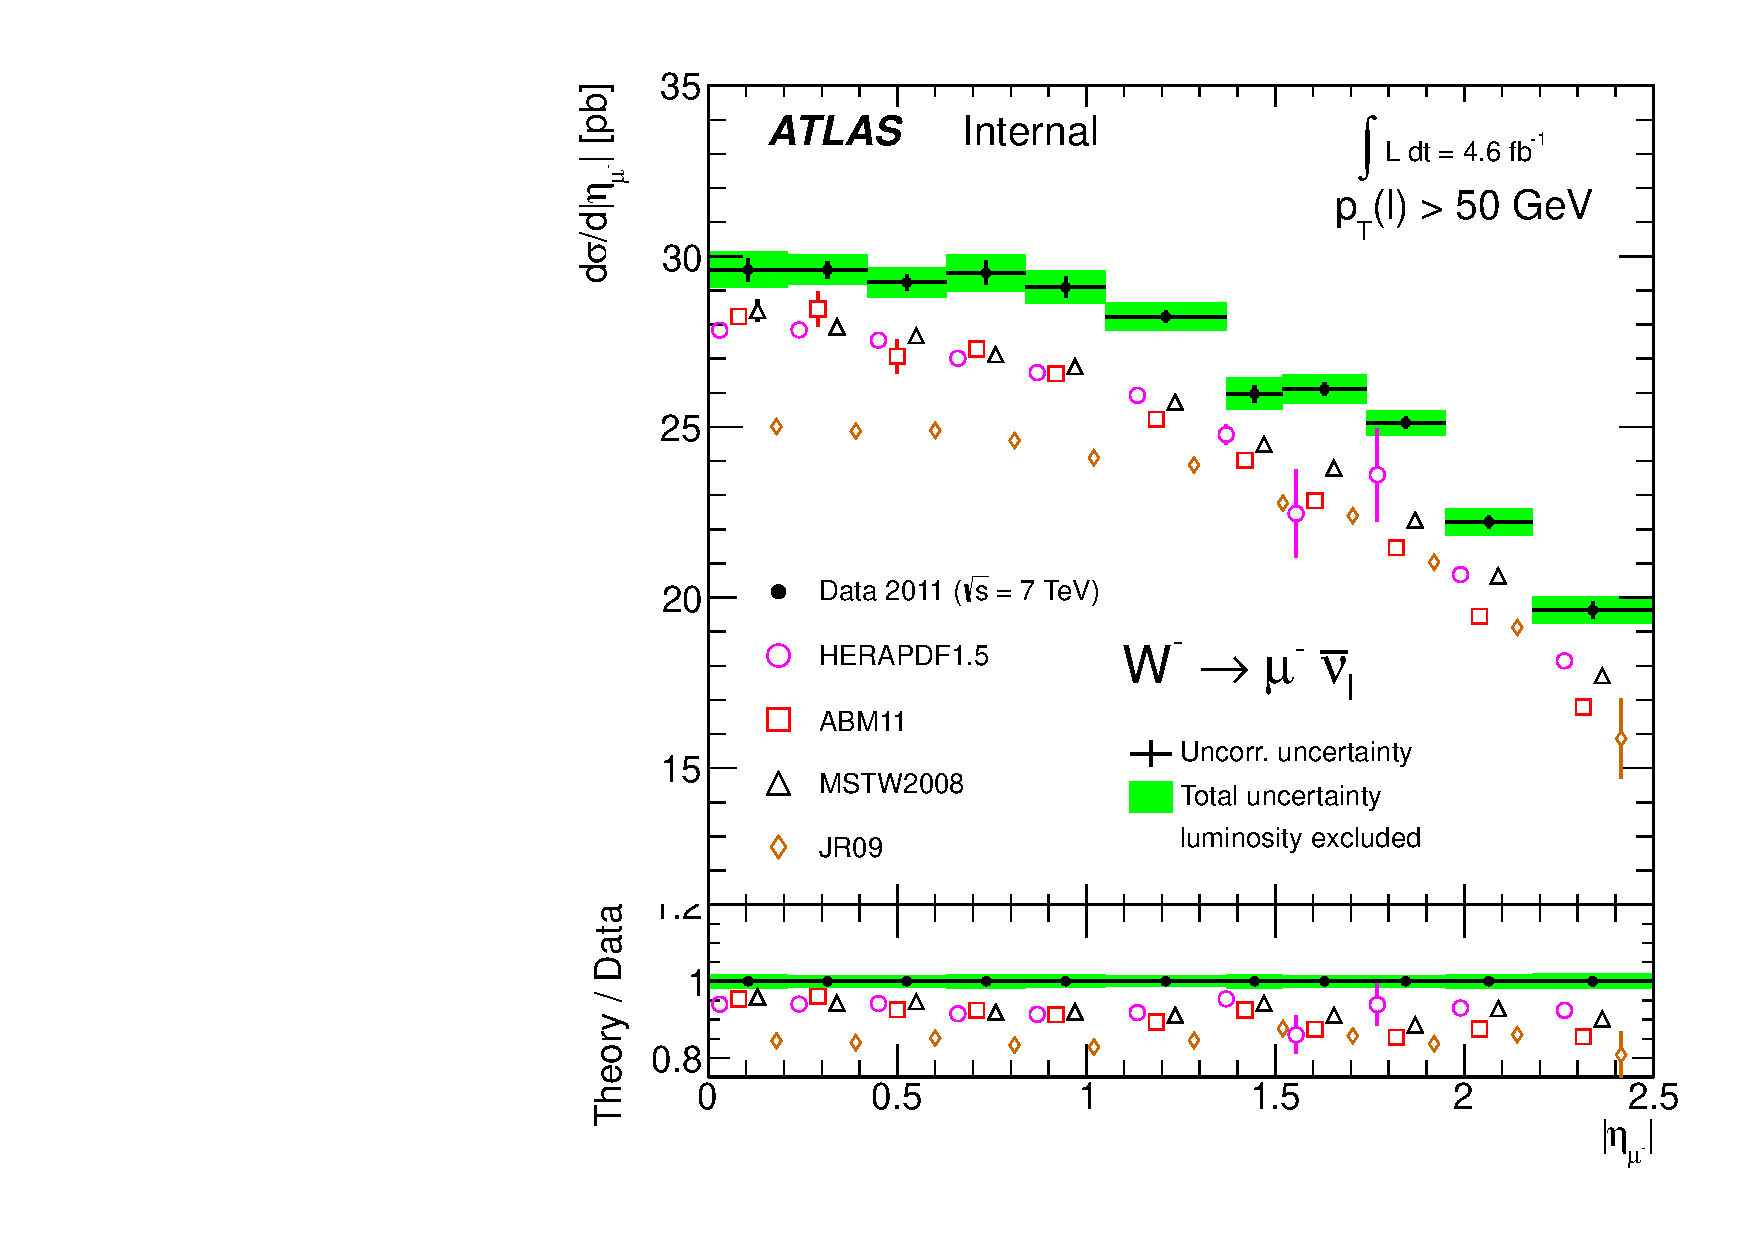
\includegraphics[width=0.55\textwidth]{res/fig/WMetaPt50_NNLO_combined}
       } 
 \caption{ The double-differential cross-section measurement for \Wminusmunu\ in $p_T$ slices: \ptFive\ and \ptSix. NNLO QCD predictions using various PDF sets (open symbols) are compared to the data (full points). The predictions are displaced within each bin for clarity. For technical reasons, the uncertainty on predictions excludes the uncertainty from the PDF error envelope. }
 \label{fig:Comb:NNLO:W2dNEG_3}
 \end{center}
\end{figure}

%% \begin{figure}[phtb]
%%   \begin{center}
%%         \subfigure[\ptOne]{%
%% 	  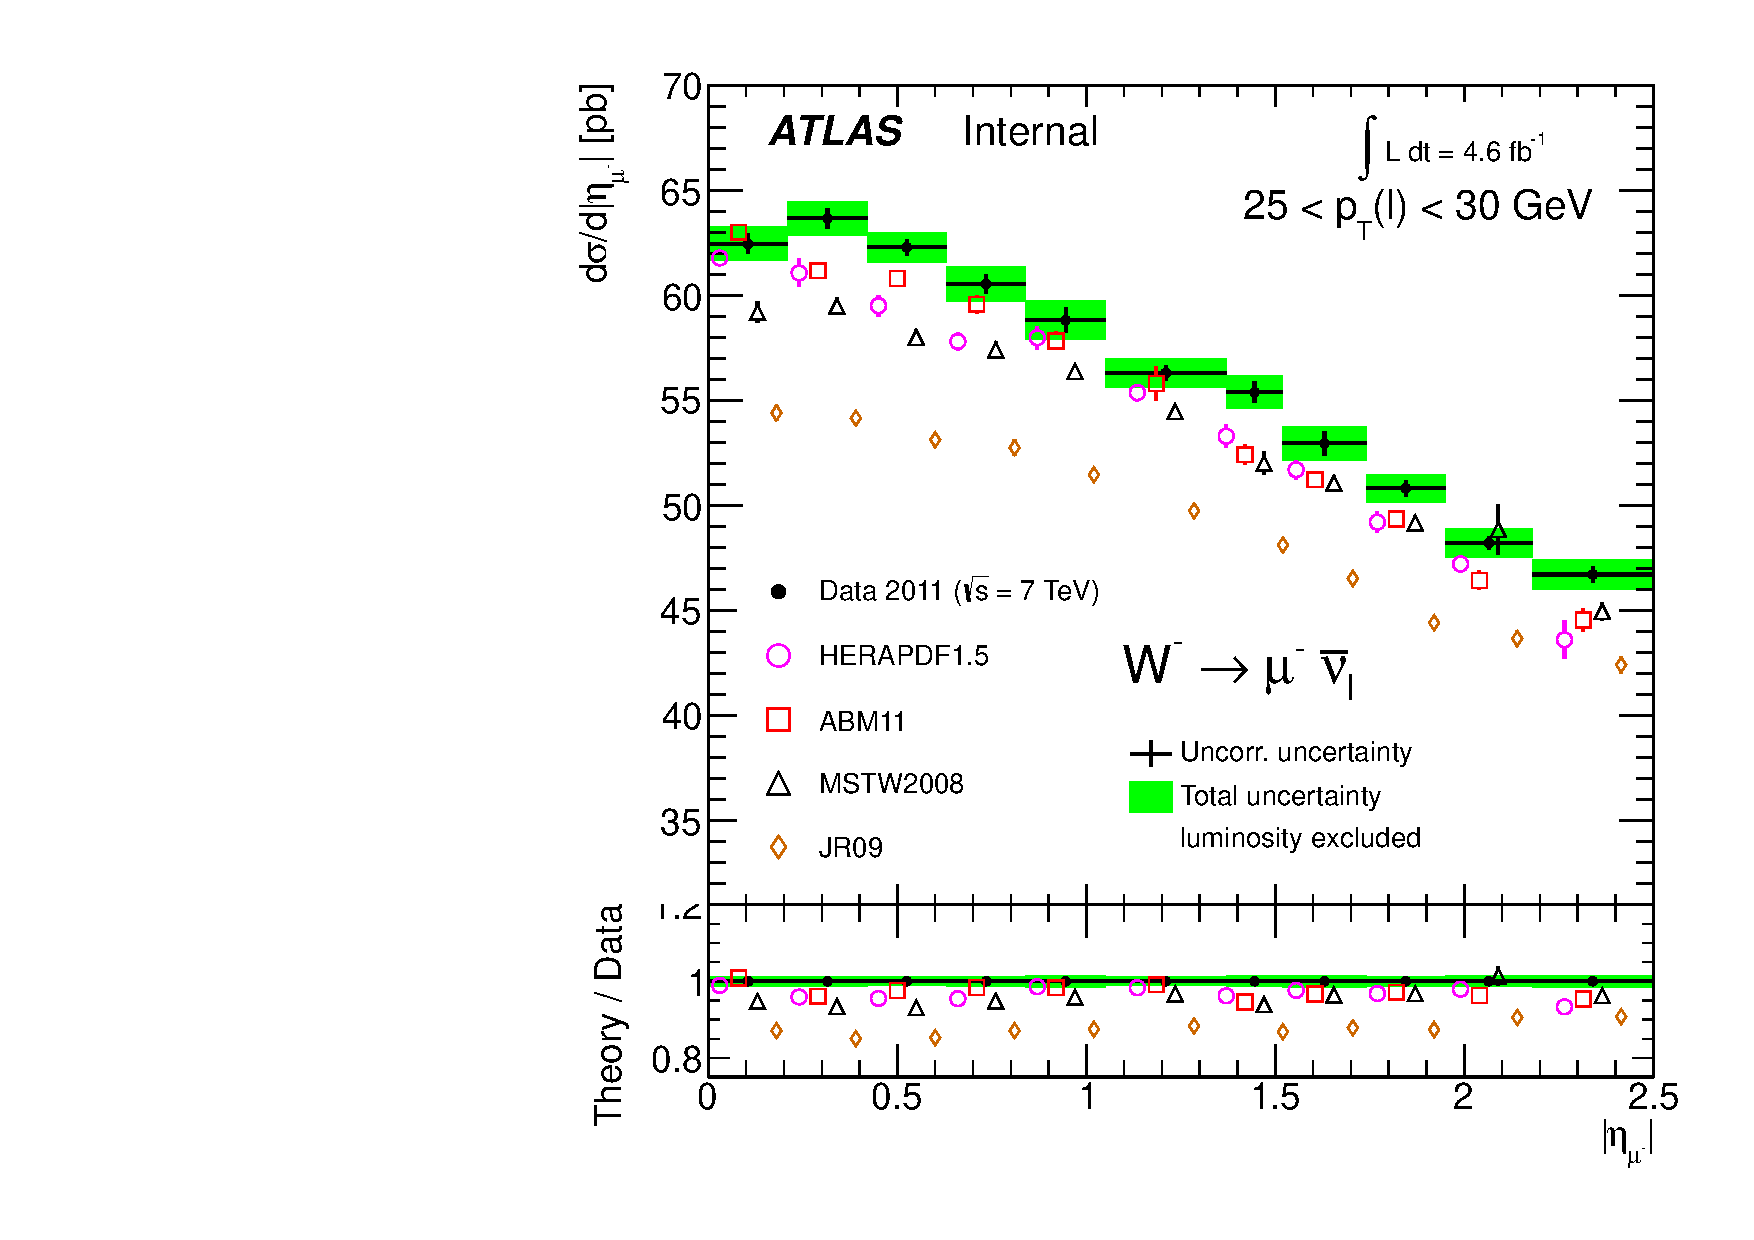
\includegraphics[width=0.36\textwidth]{res/fig/WMetaPt25_30_NNLO_combined}
%%         }
%%        \subfigure[\ptTwo]{%
%% 	  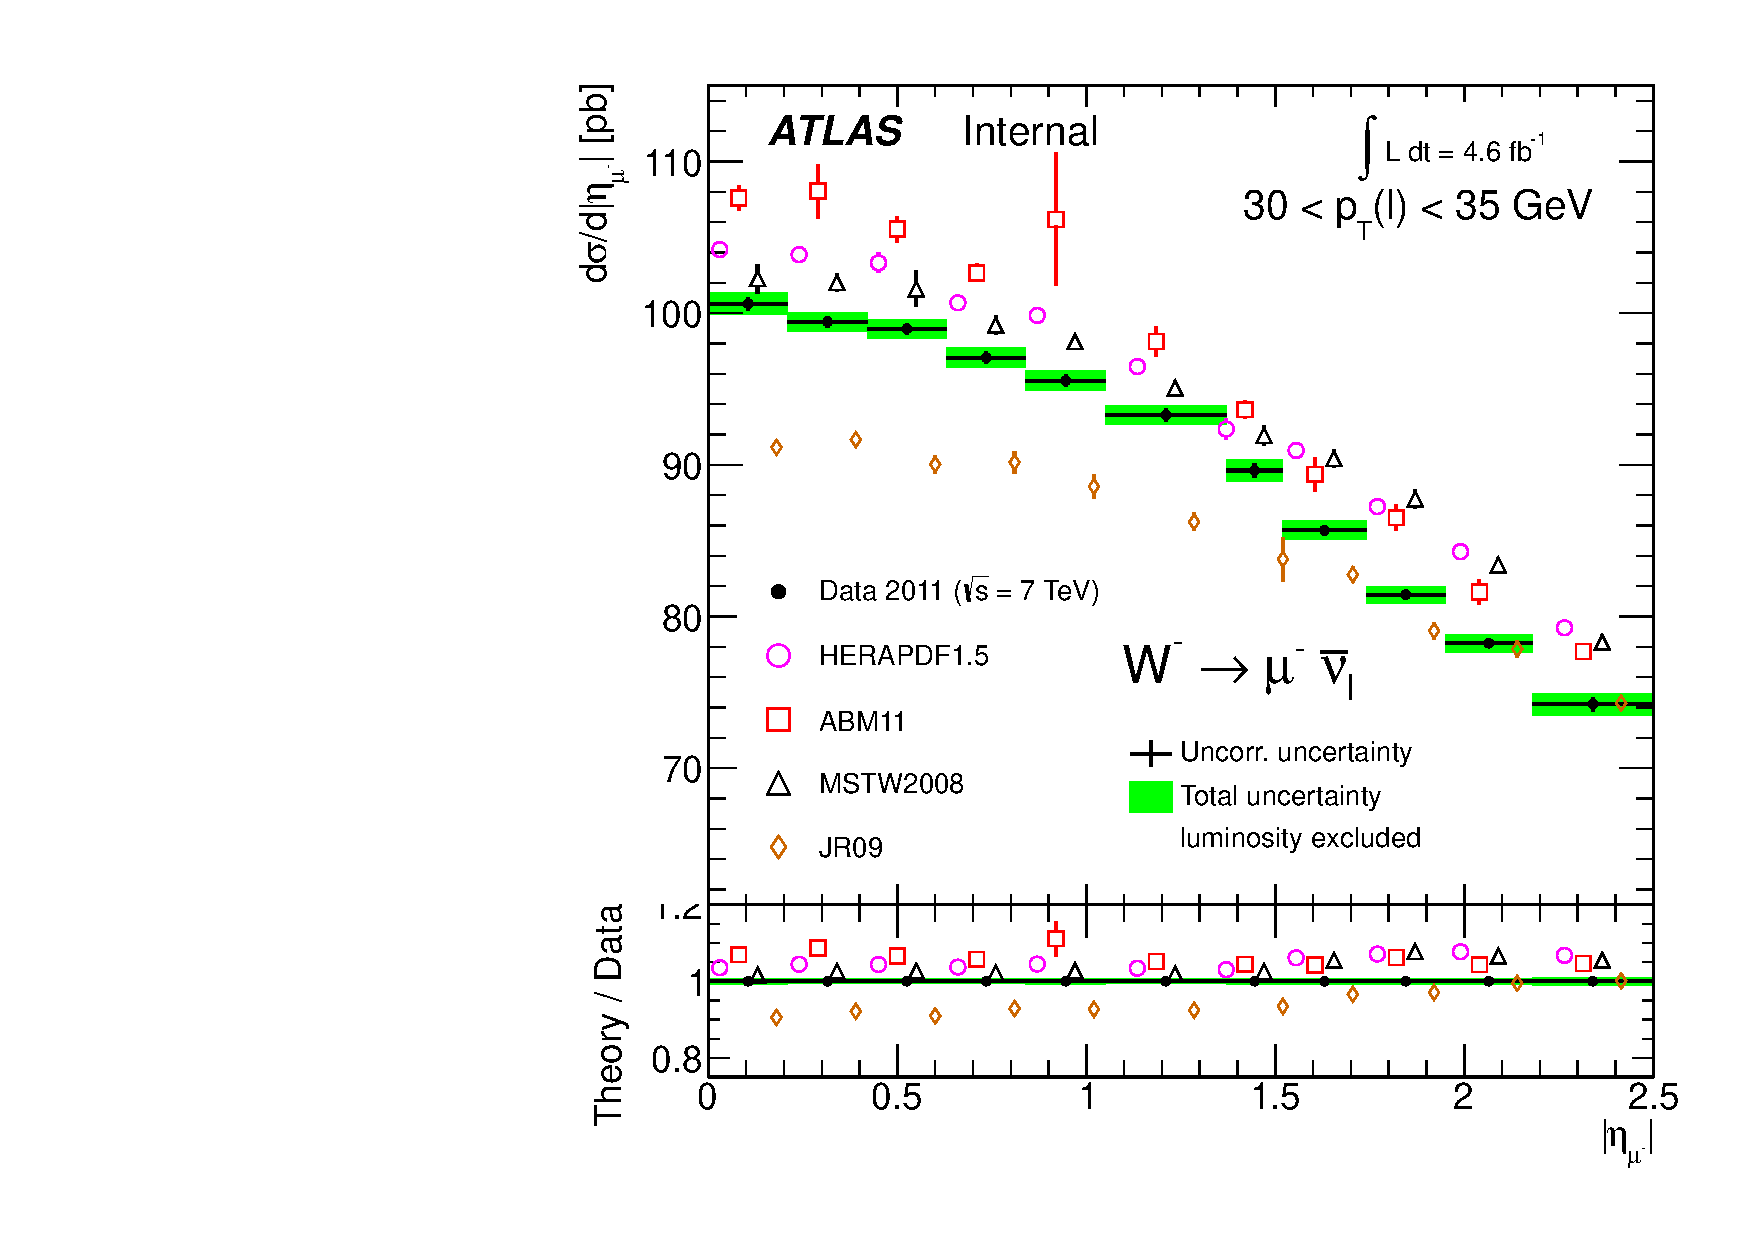
\includegraphics[width=0.36\textwidth]{res/fig/WMetaPt30_35_NNLO_combined}
%%         } \\
%%        \subfigure[\ptThree]{%
%% 	  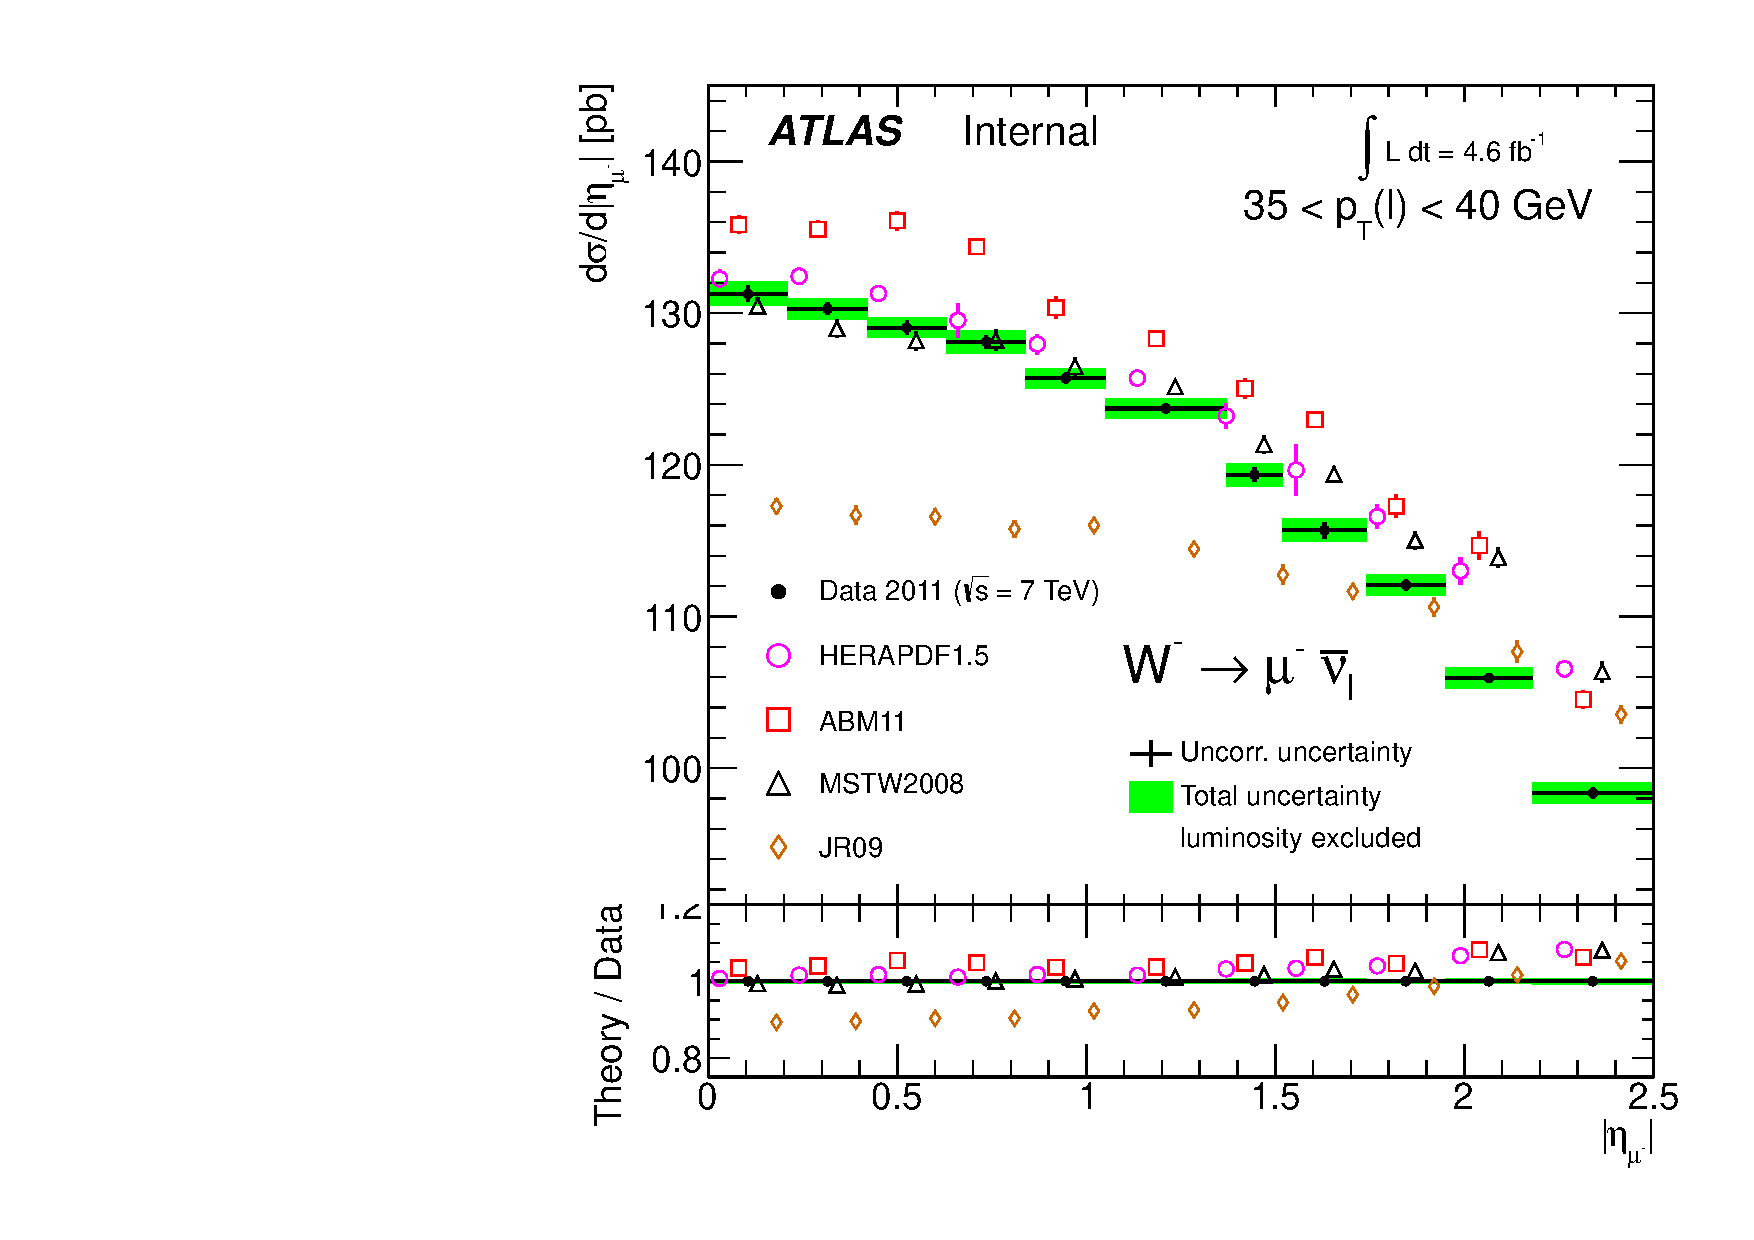
\includegraphics[width=0.36\textwidth]{res/fig/WMetaPt35_40_NNLO_combined}
%%         }
%%        \subfigure[\ptFour]{%
%% 	  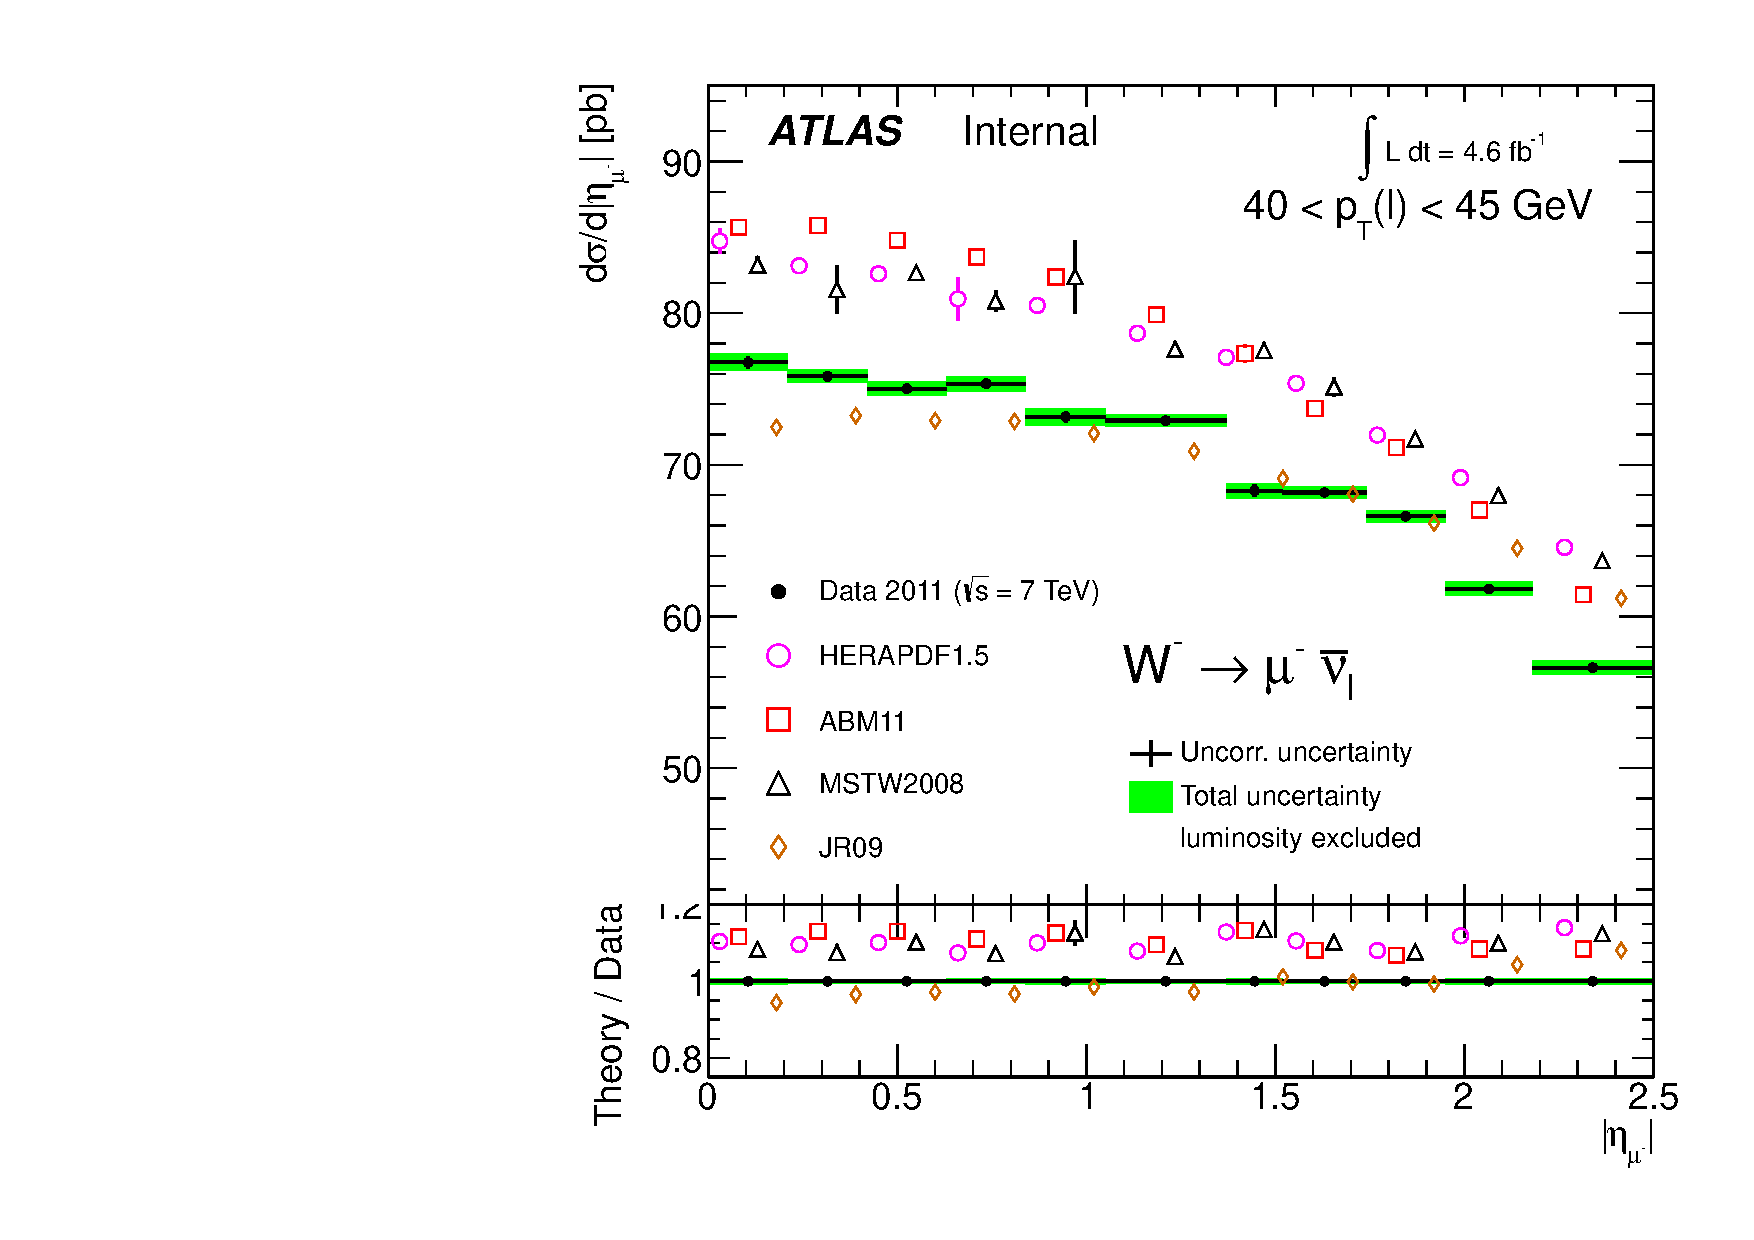
\includegraphics[width=0.36\textwidth]{res/fig/WMetaPt40_45_NNLO_combined}
%%         } \\
%%        \subfigure[\ptFive]{%
%% 	  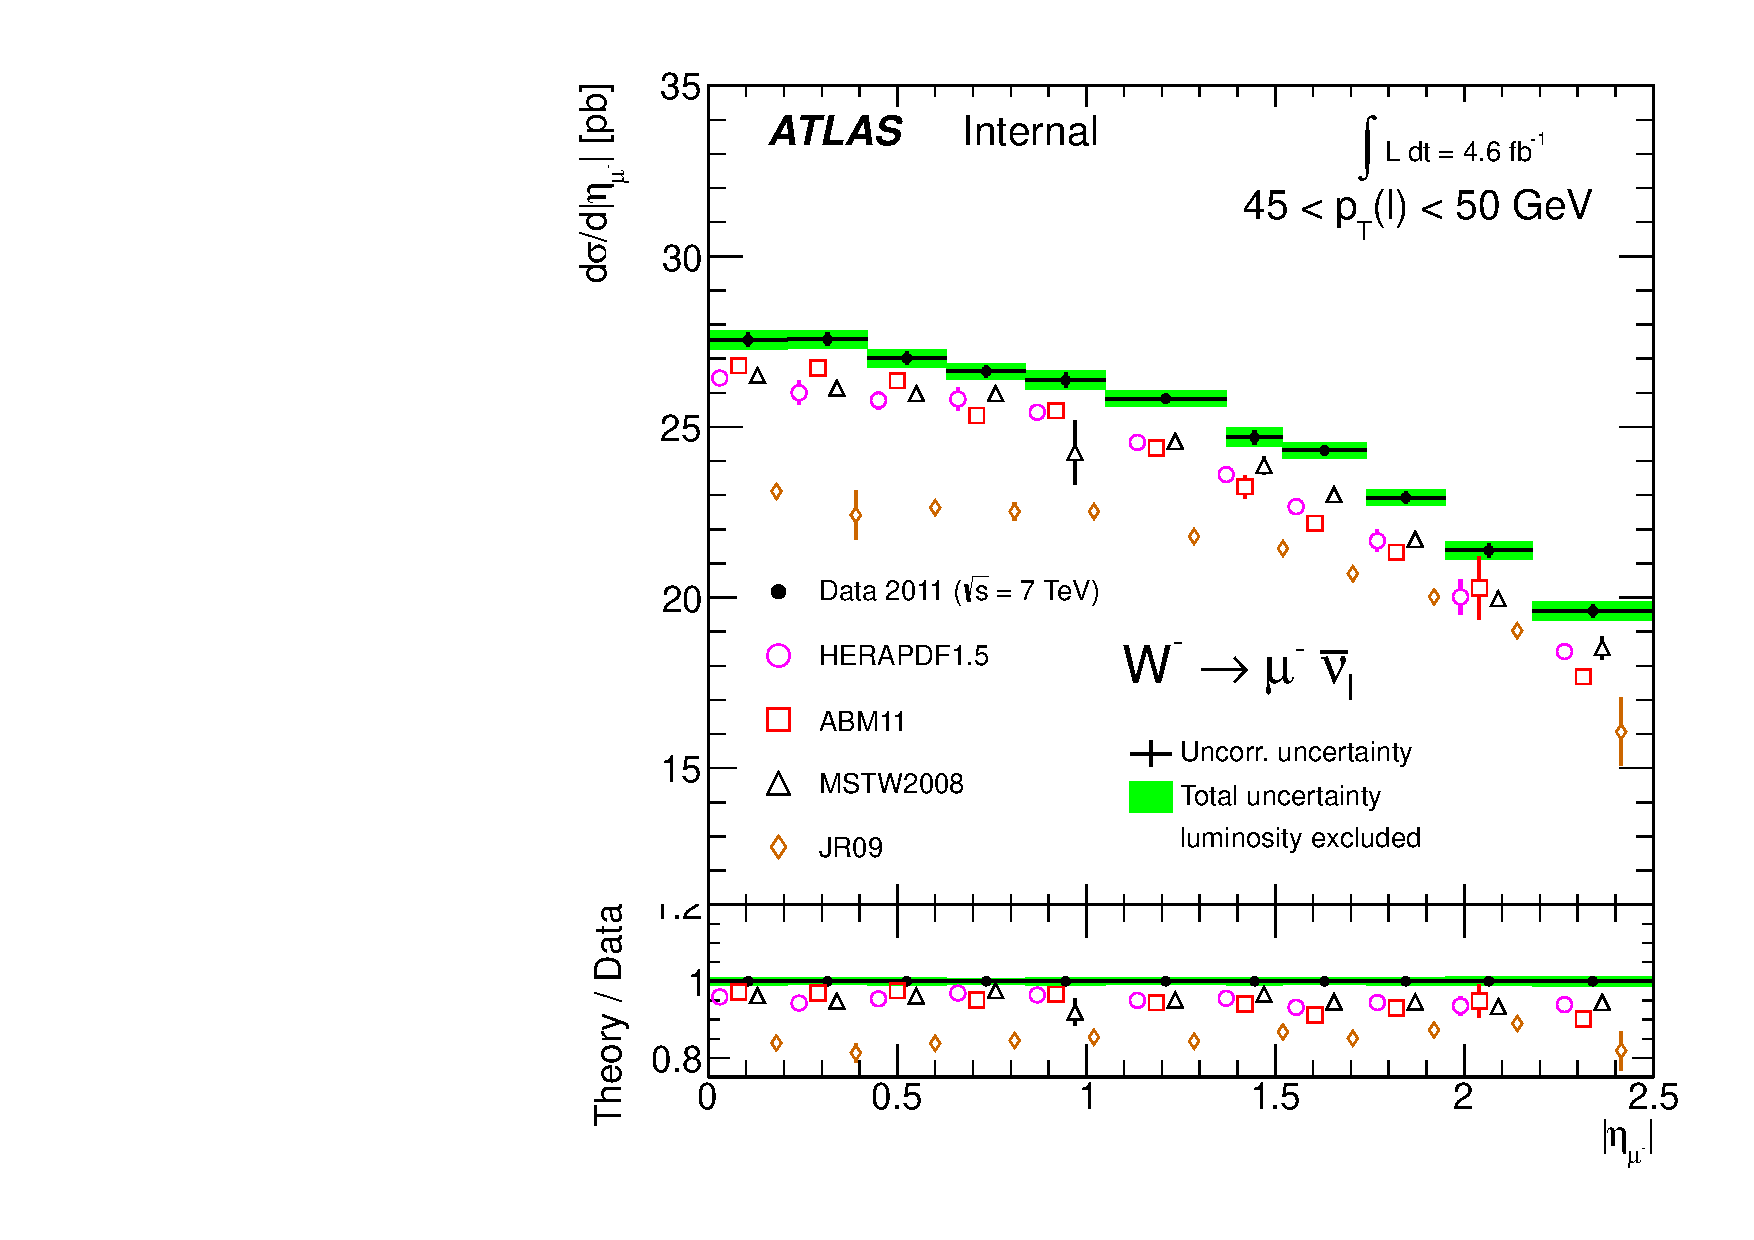
\includegraphics[width=0.36\textwidth]{res/fig/WMetaPt45_50_NNLO_combined}
%%         }
%%        \subfigure[\ptSix]{%
%% 	  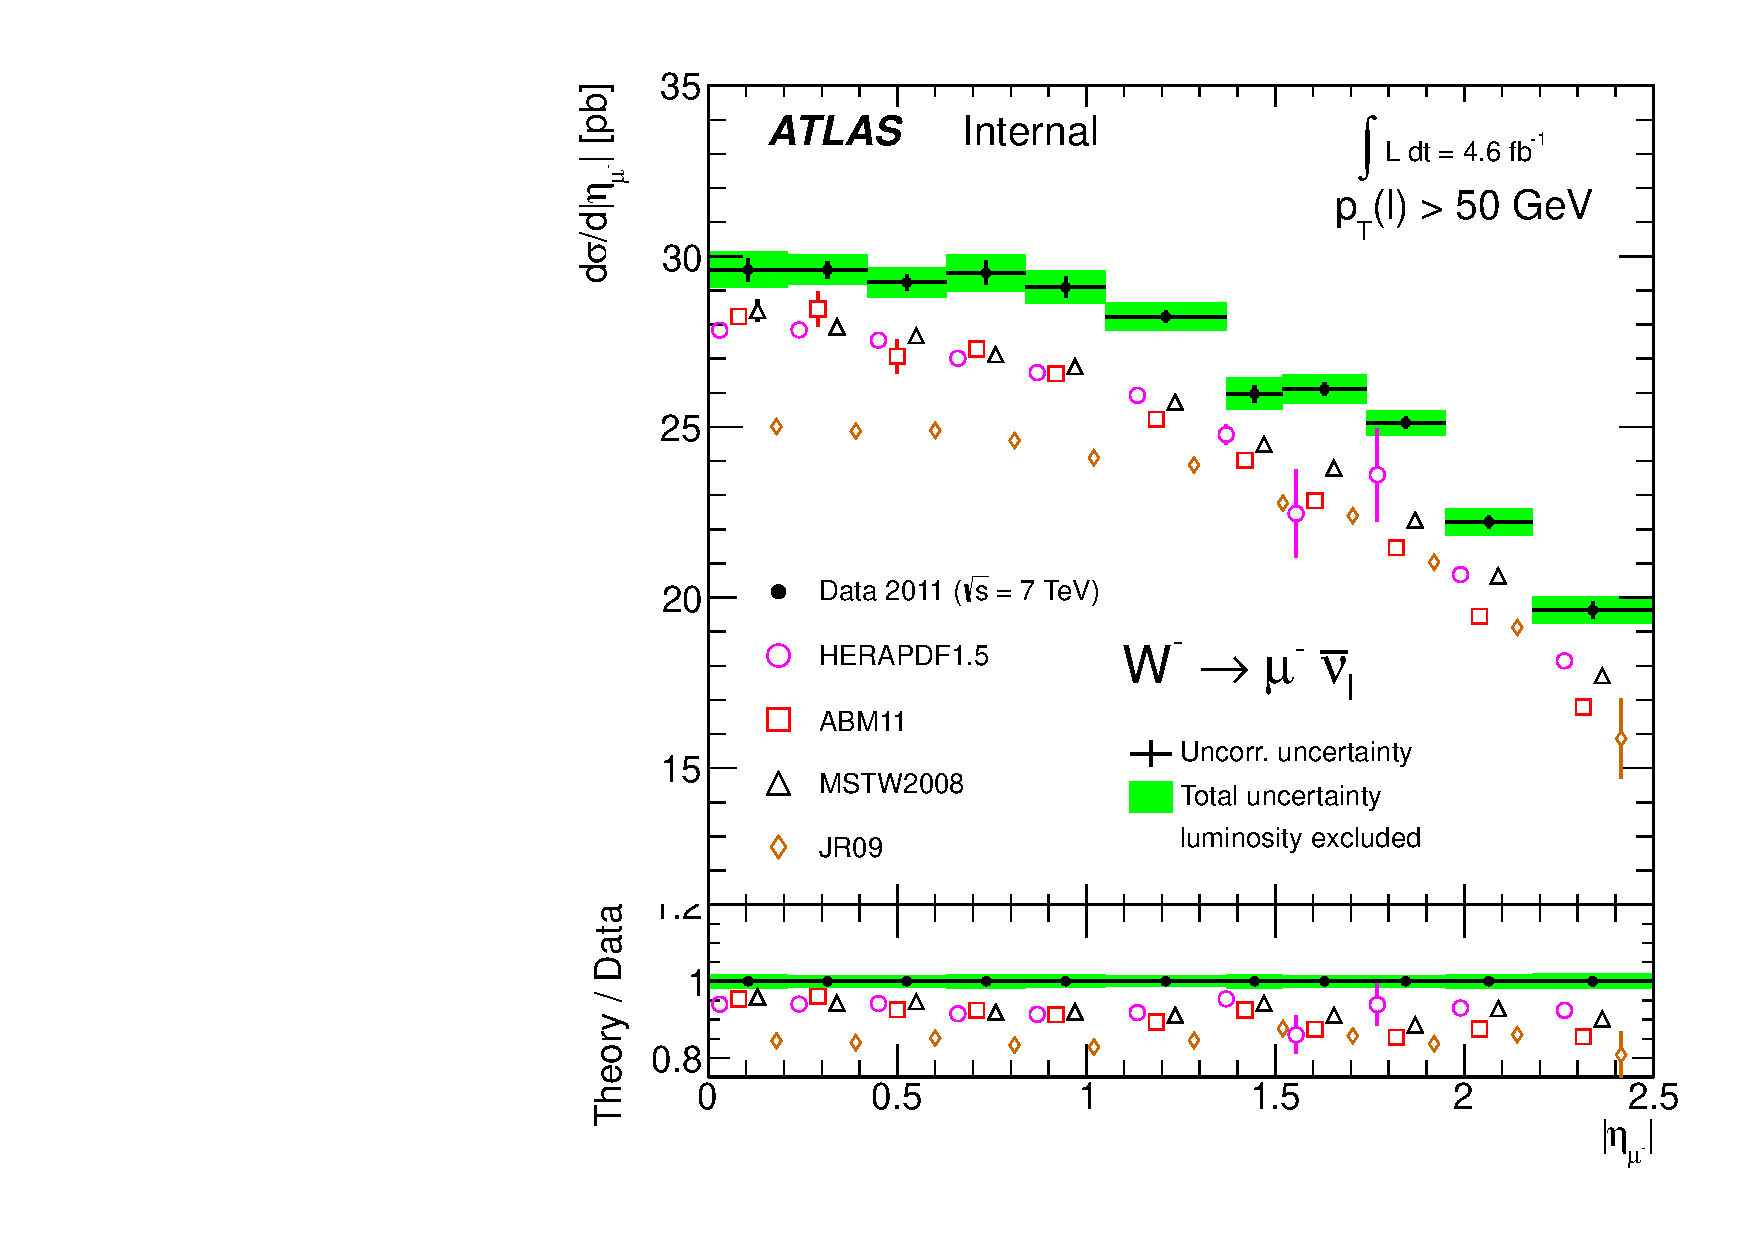
\includegraphics[width=0.36\textwidth]{res/fig/WMetaPt50_NNLO_combined}
%%        } 
%%  \caption{ The double-differential cross-section measurement for \Wminusmunu\ in $p_T$ slices. NNLO QCD predictions using various PDF sets (open symbols) are compared to the data (full points). The predictions are displaced within each bin for clarity. For technical reasons, the uncertainty on predictions excludes the uncertainty from the PDF error envelope. }
%%  \label{fig:Comb:NNLO:W2dNEG}
%%  \end{center}
%% \end{figure}

\begin{figure}[phtb]
  \begin{center}
        \subfigure[\ptOne]{%
	  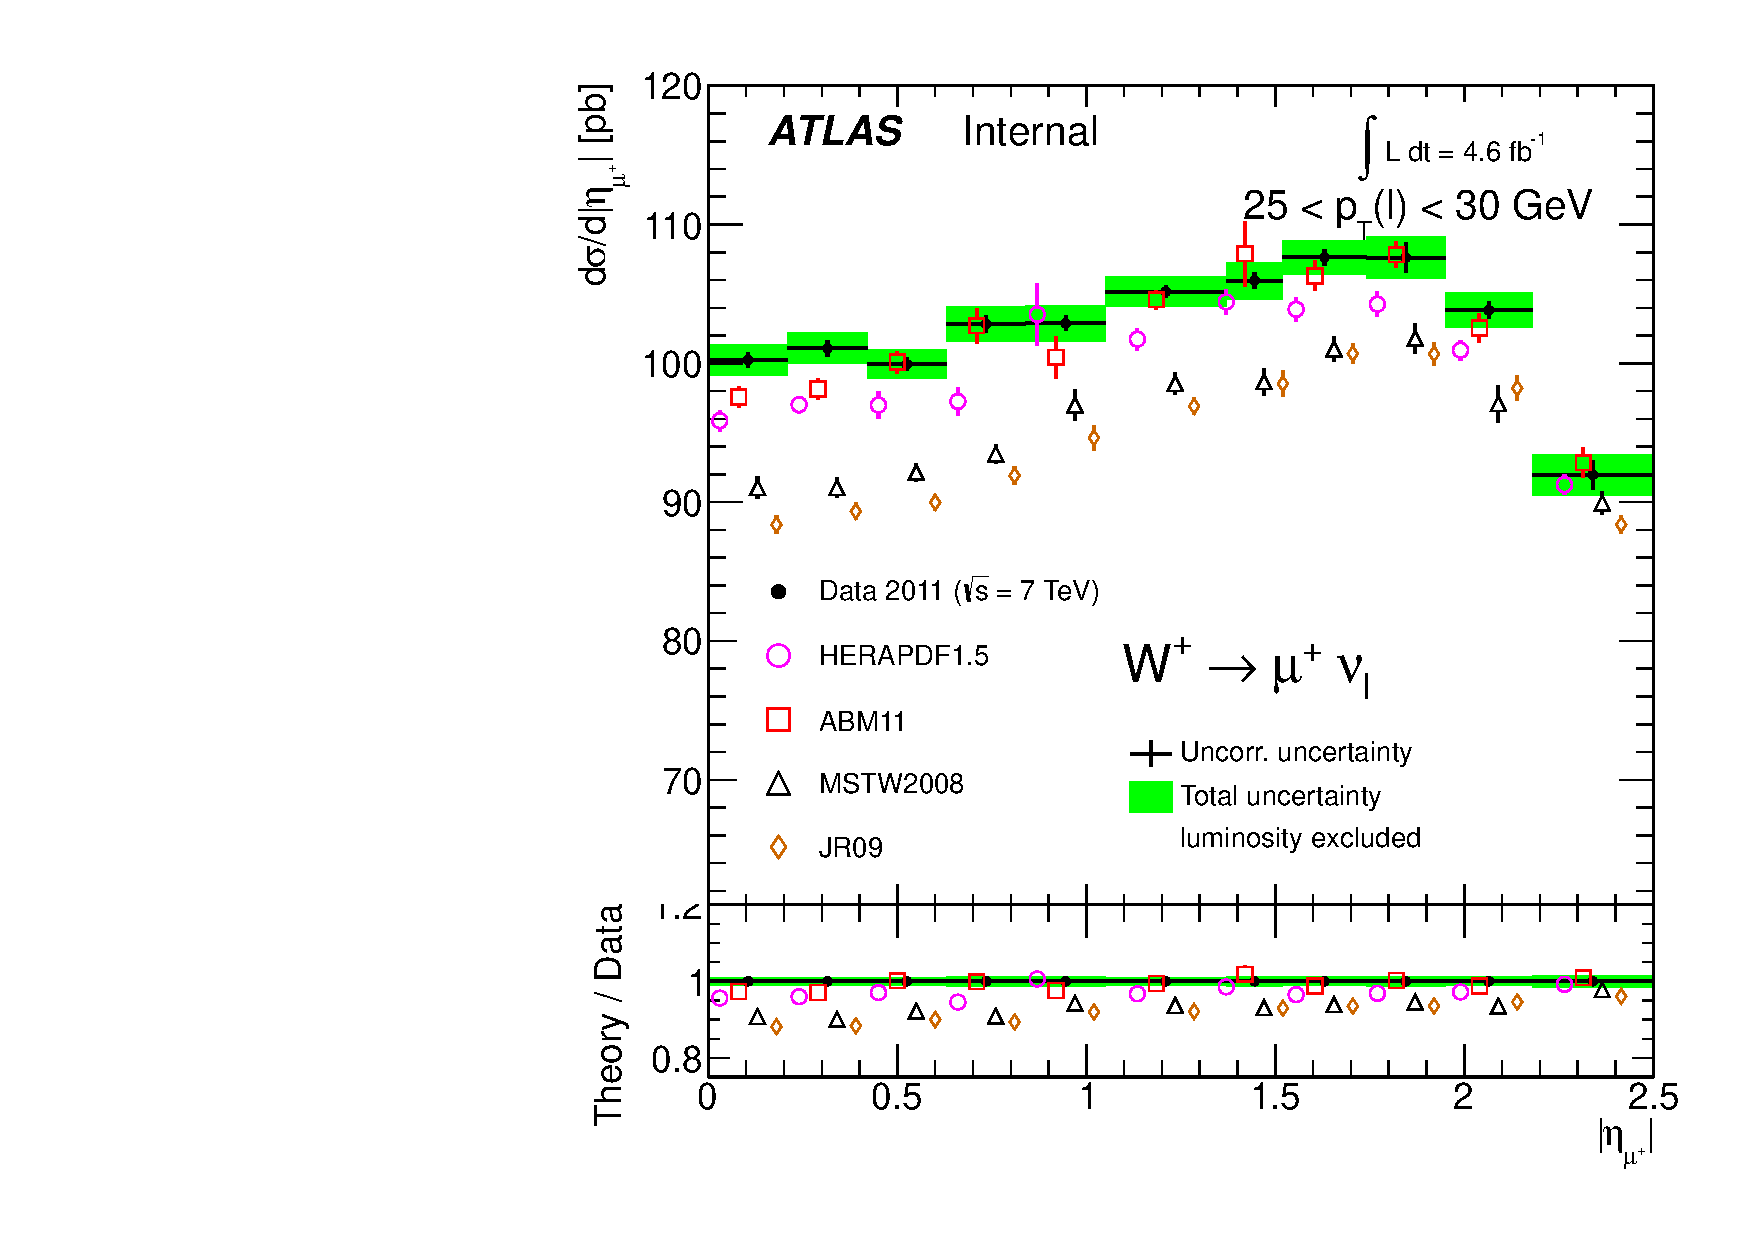
\includegraphics[width=0.55\textwidth]{res/fig/WPetaPt25_30_NNLO_combined}
        }
       \subfigure[\ptTwo]{%
	  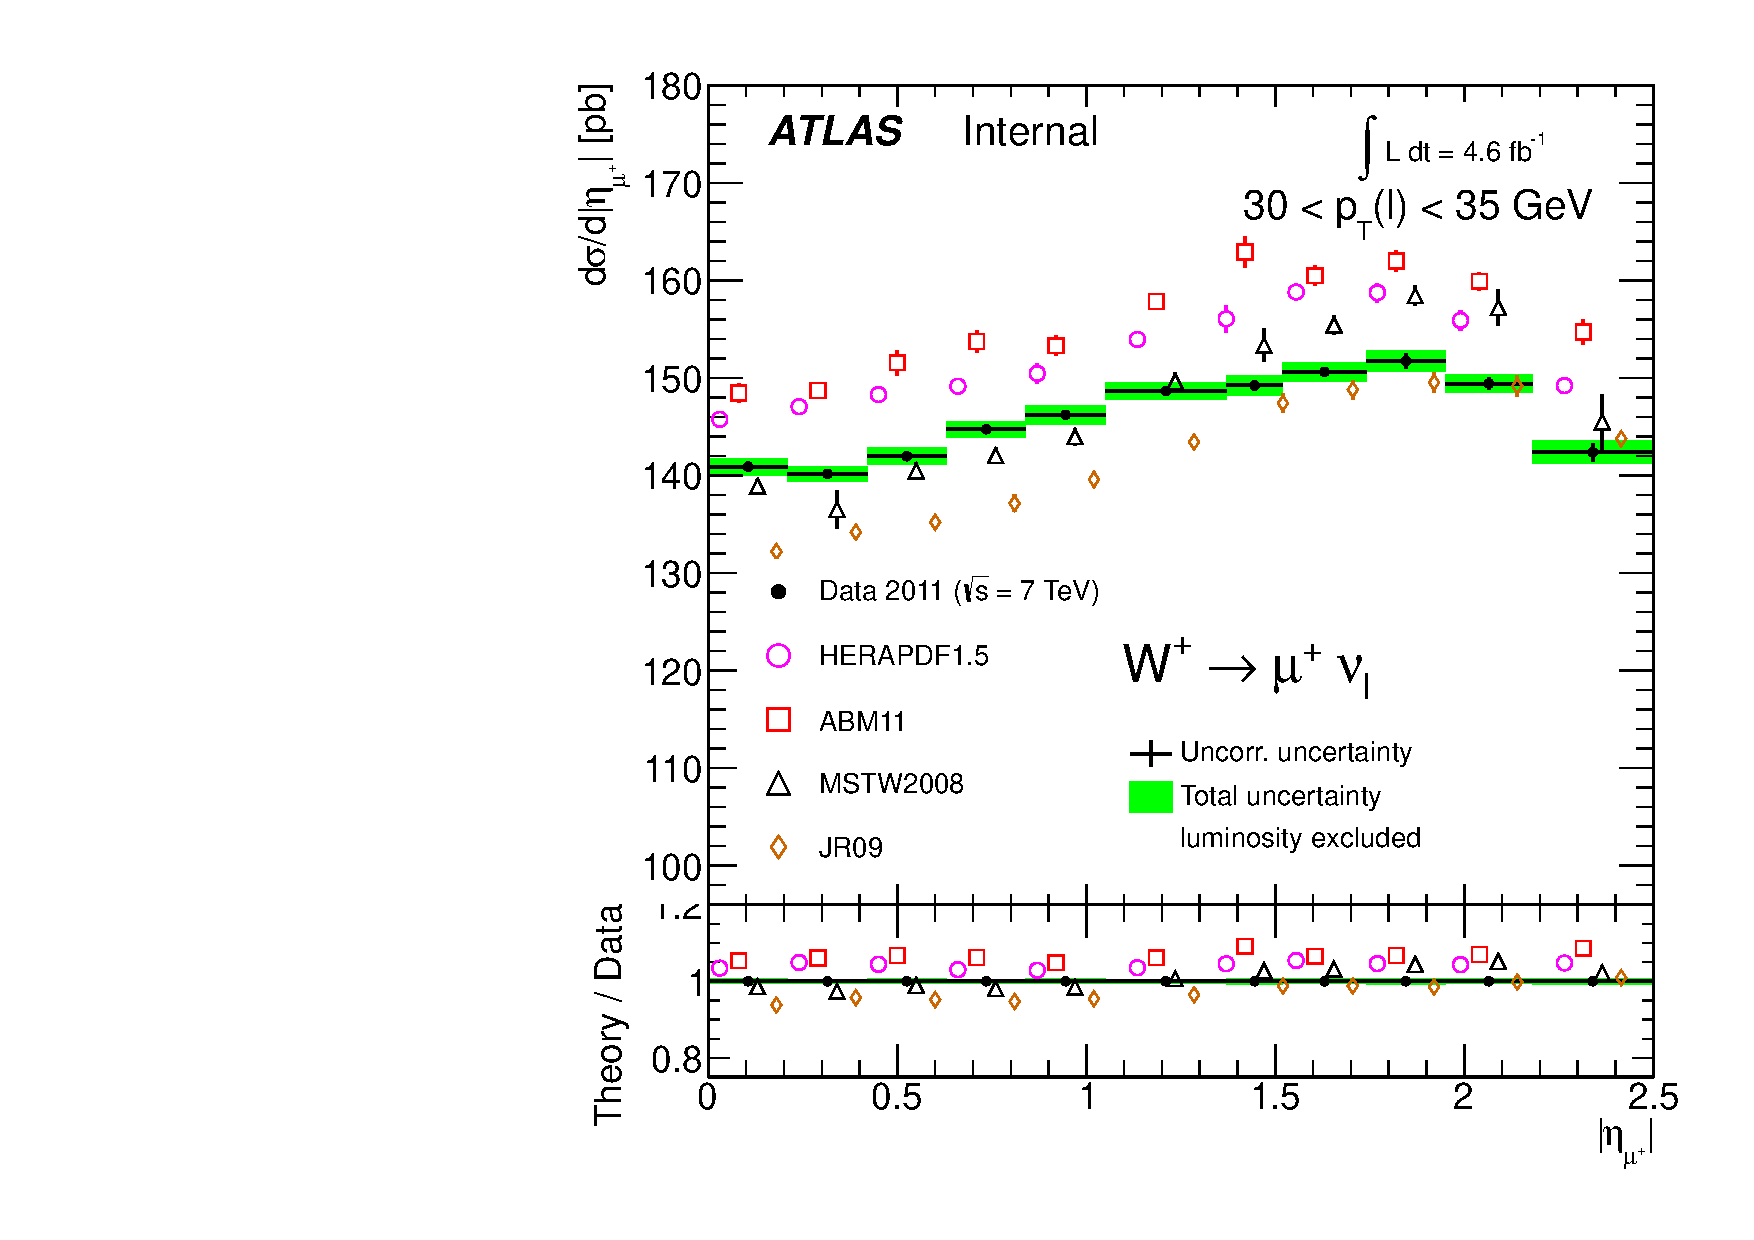
\includegraphics[width=0.55\textwidth]{res/fig/WPetaPt30_35_NNLO_combined}
        }
 \caption{ The double-differential cross-section measurement for \Wplusmunu\ in $p_T$ slices: \ptOne\ and \ptTwo. NNLO QCD predictions using various PDF sets (open symbols) are compared to the data (full points). For technical reasons, the uncertainty on predictions excludes the uncertainty from the PDF error envelope. }
 \label{fig:Comb:NNLO:W2dPOS_1}
 \end{center}
\end{figure}

\begin{figure}[phtb]
  \begin{center}
       \subfigure[\ptThree]{%
	  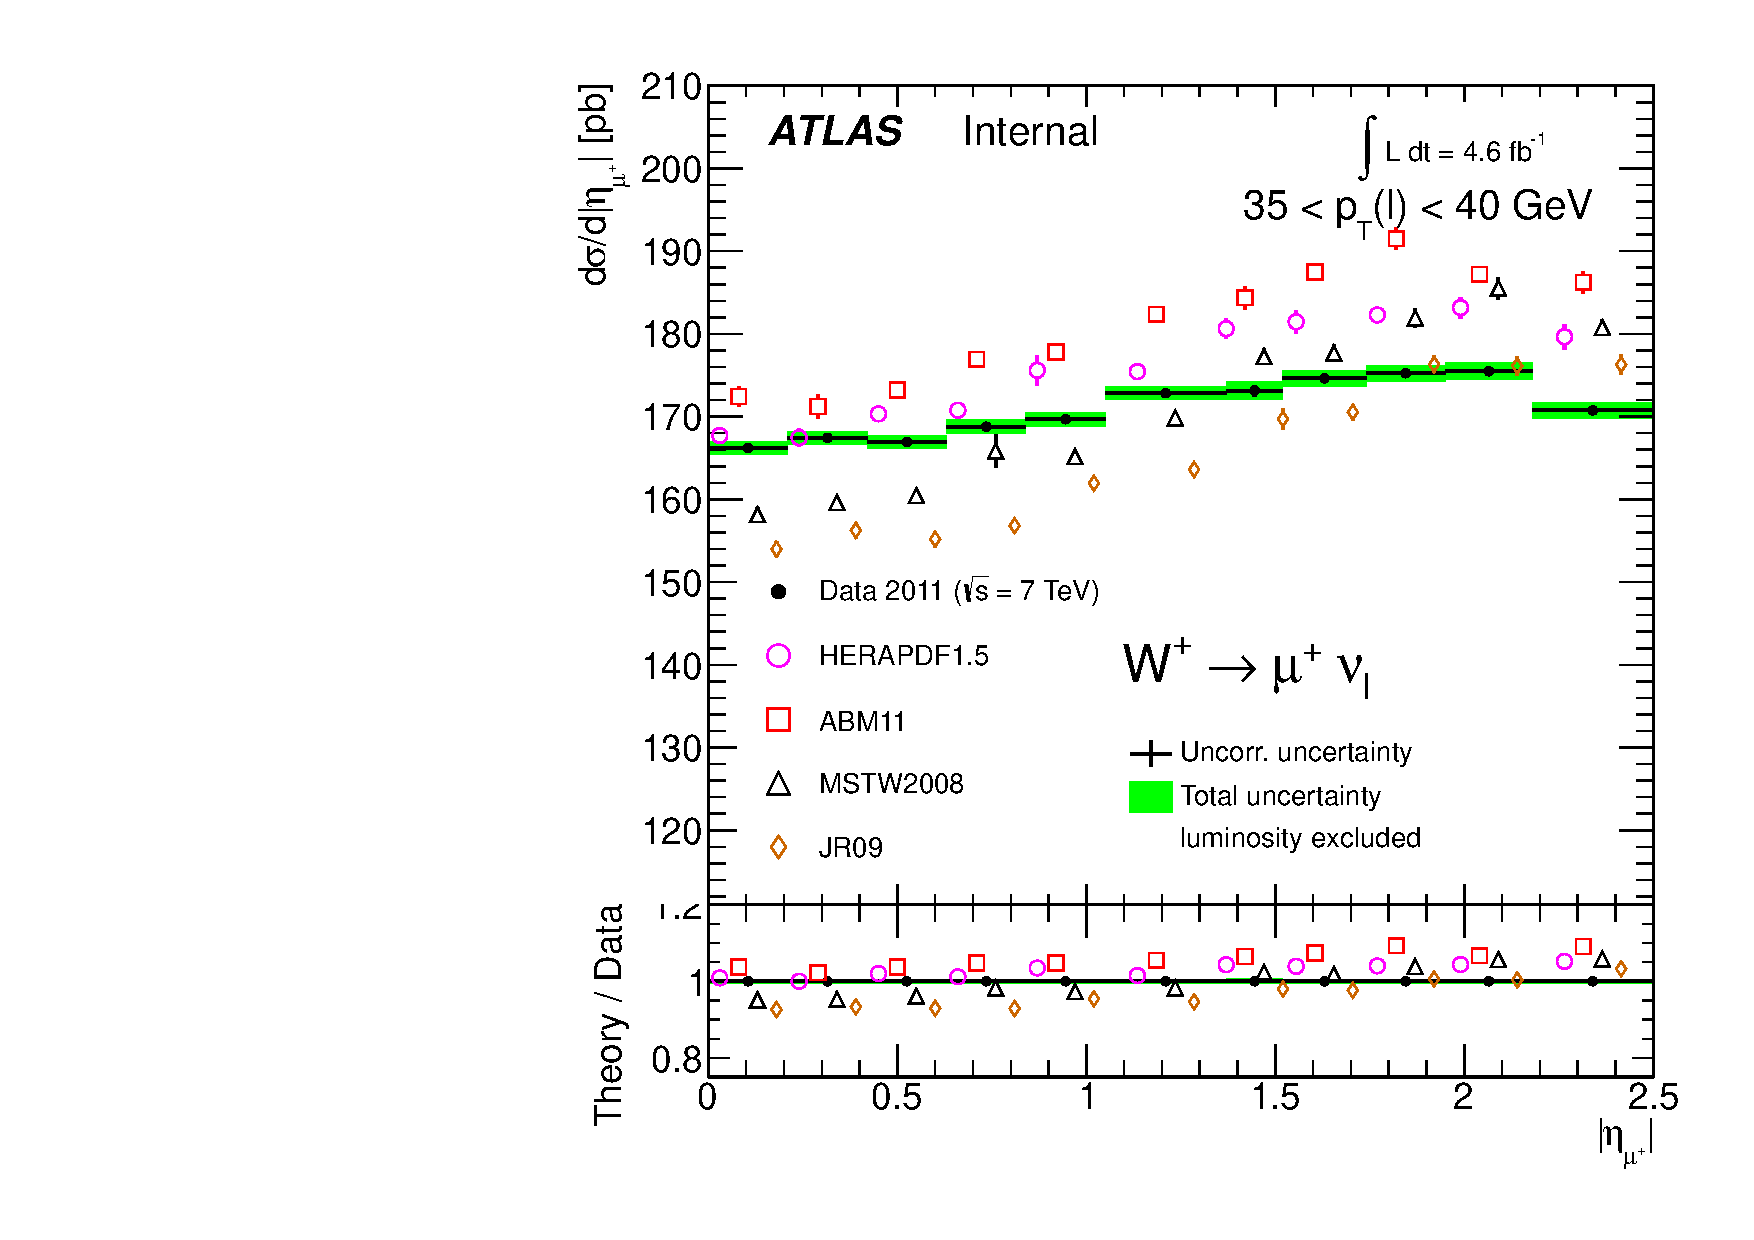
\includegraphics[width=0.55\textwidth]{res/fig/WPetaPt35_40_NNLO_combined}
        }
       \subfigure[\ptFour]{%
	  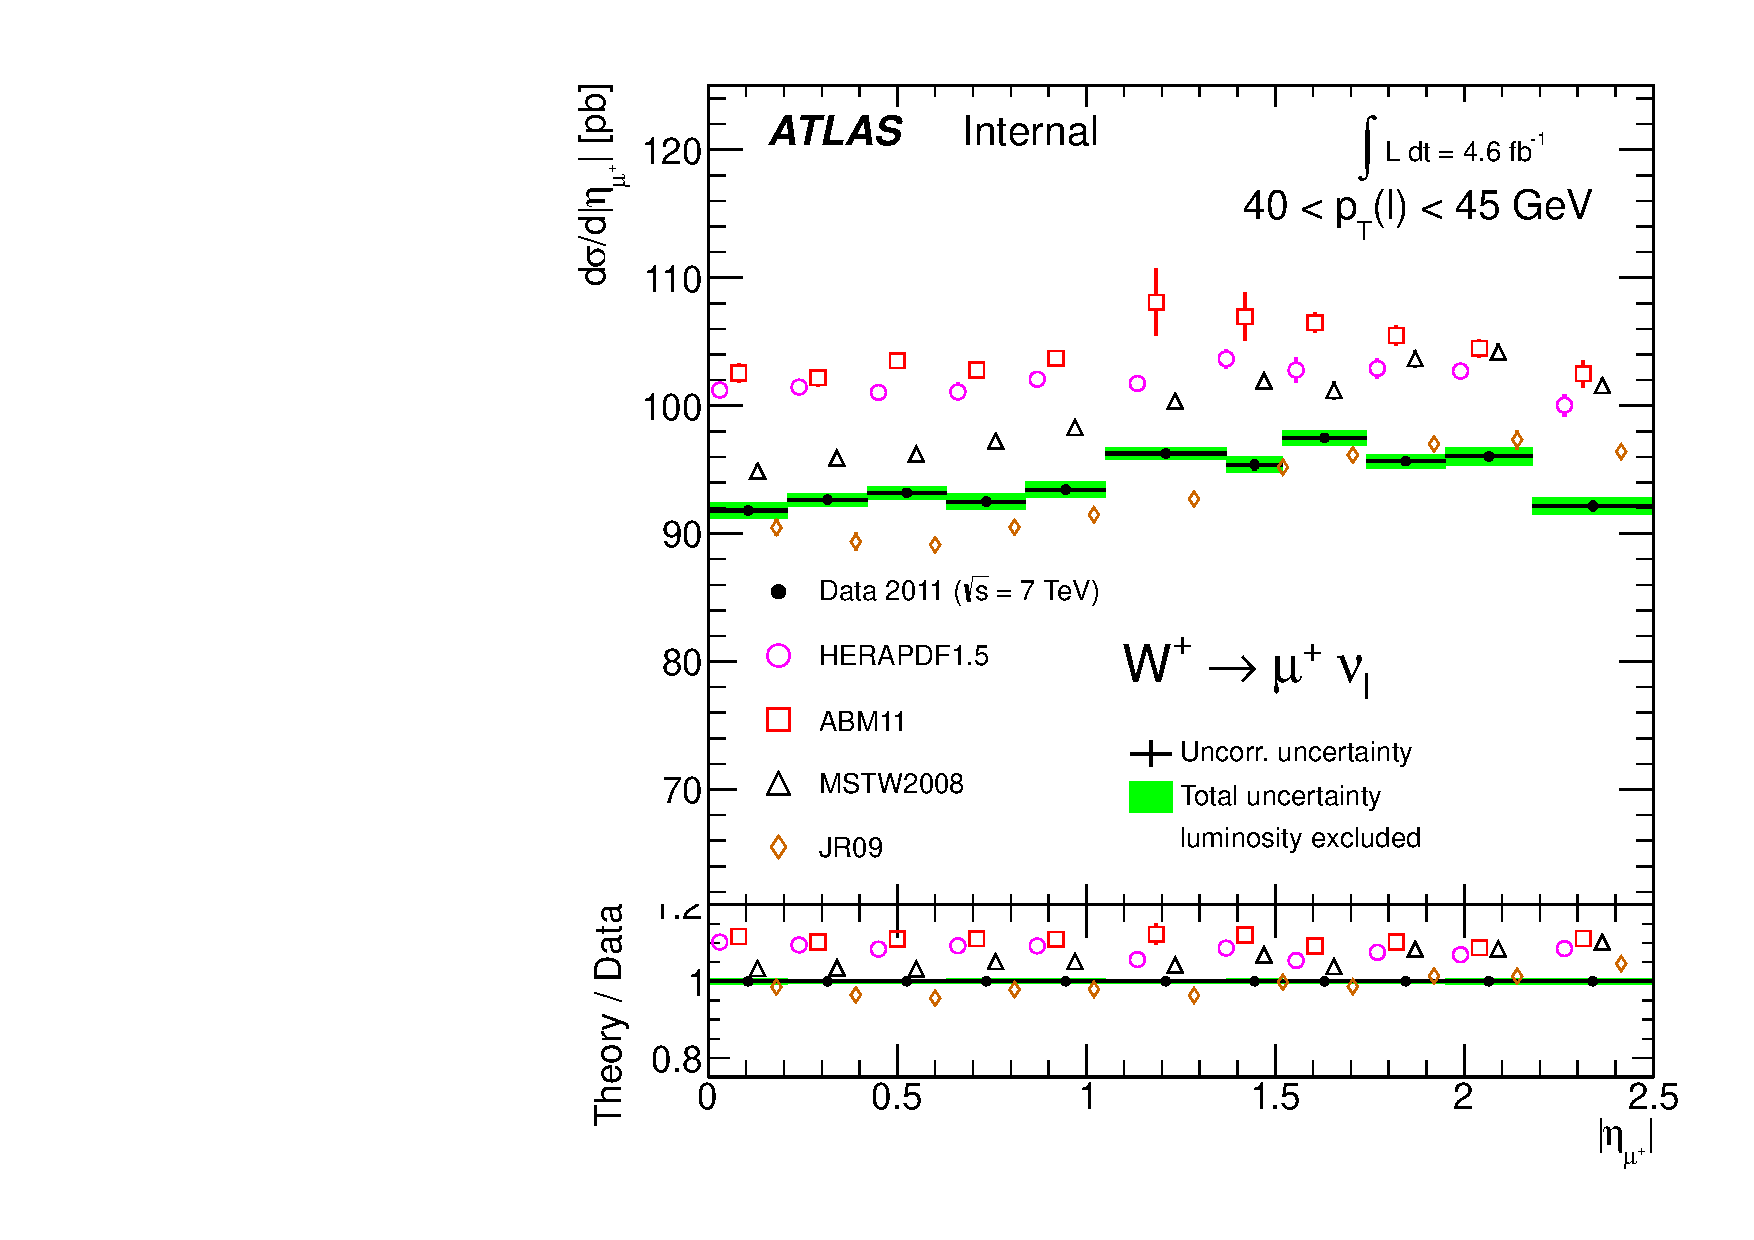
\includegraphics[width=0.55\textwidth]{res/fig/WPetaPt40_45_NNLO_combined}
        }
 \caption{ The double-differential cross-section measurement for \Wplusmunu\ in $p_T$ slices: \ptThree\ and \ptFour. NNLO QCD predictions using various PDF sets (open symbols) are compared to the data (full points). For technical reasons, the uncertainty on predictions excludes the uncertainty from the PDF error envelope. }
 \label{fig:Comb:NNLO:W2dPOS_2}
 \end{center}
\end{figure}

\begin{figure}[phtb]
  \begin{center}
       \subfigure[\ptFive]{%
	  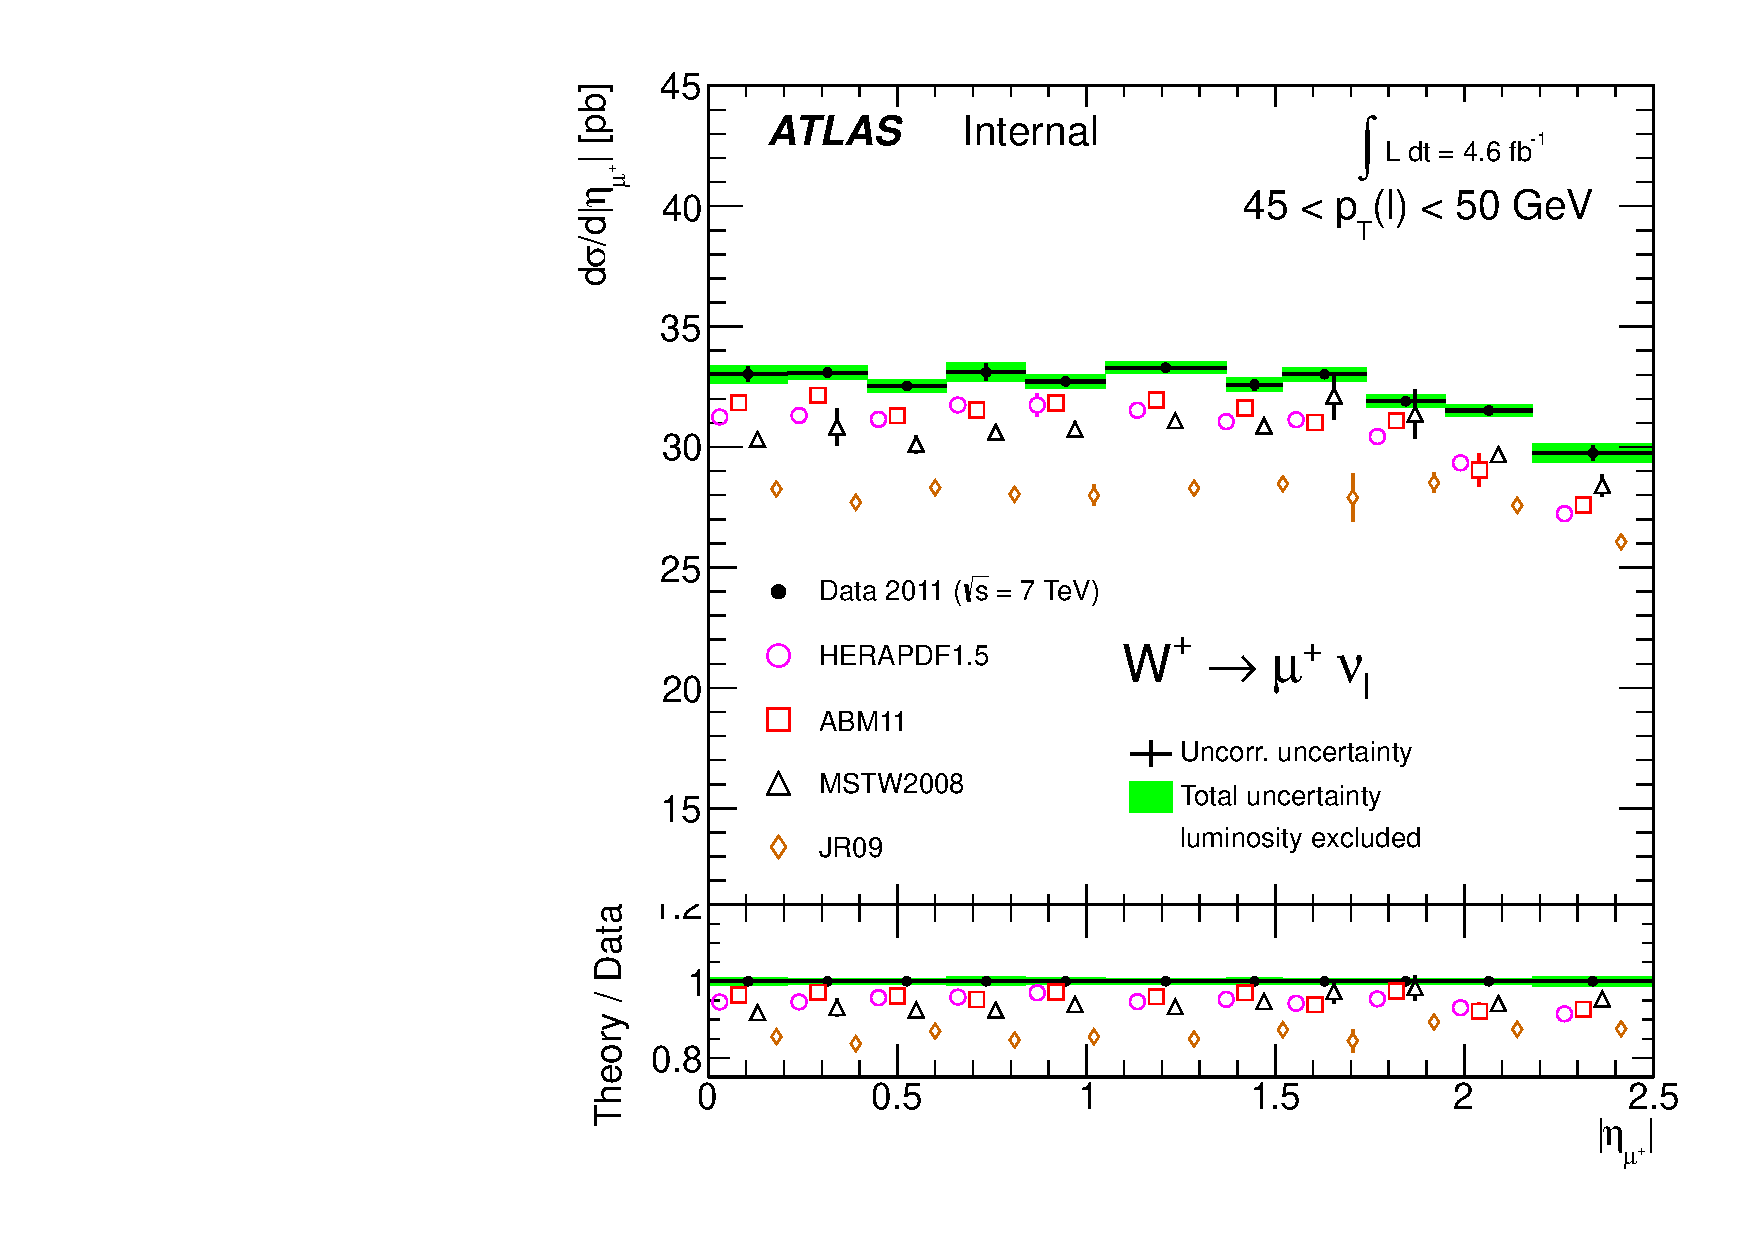
\includegraphics[width=0.55\textwidth]{res/fig/WPetaPt45_50_NNLO_combined}
        }
       \subfigure[\ptSix]{%
	  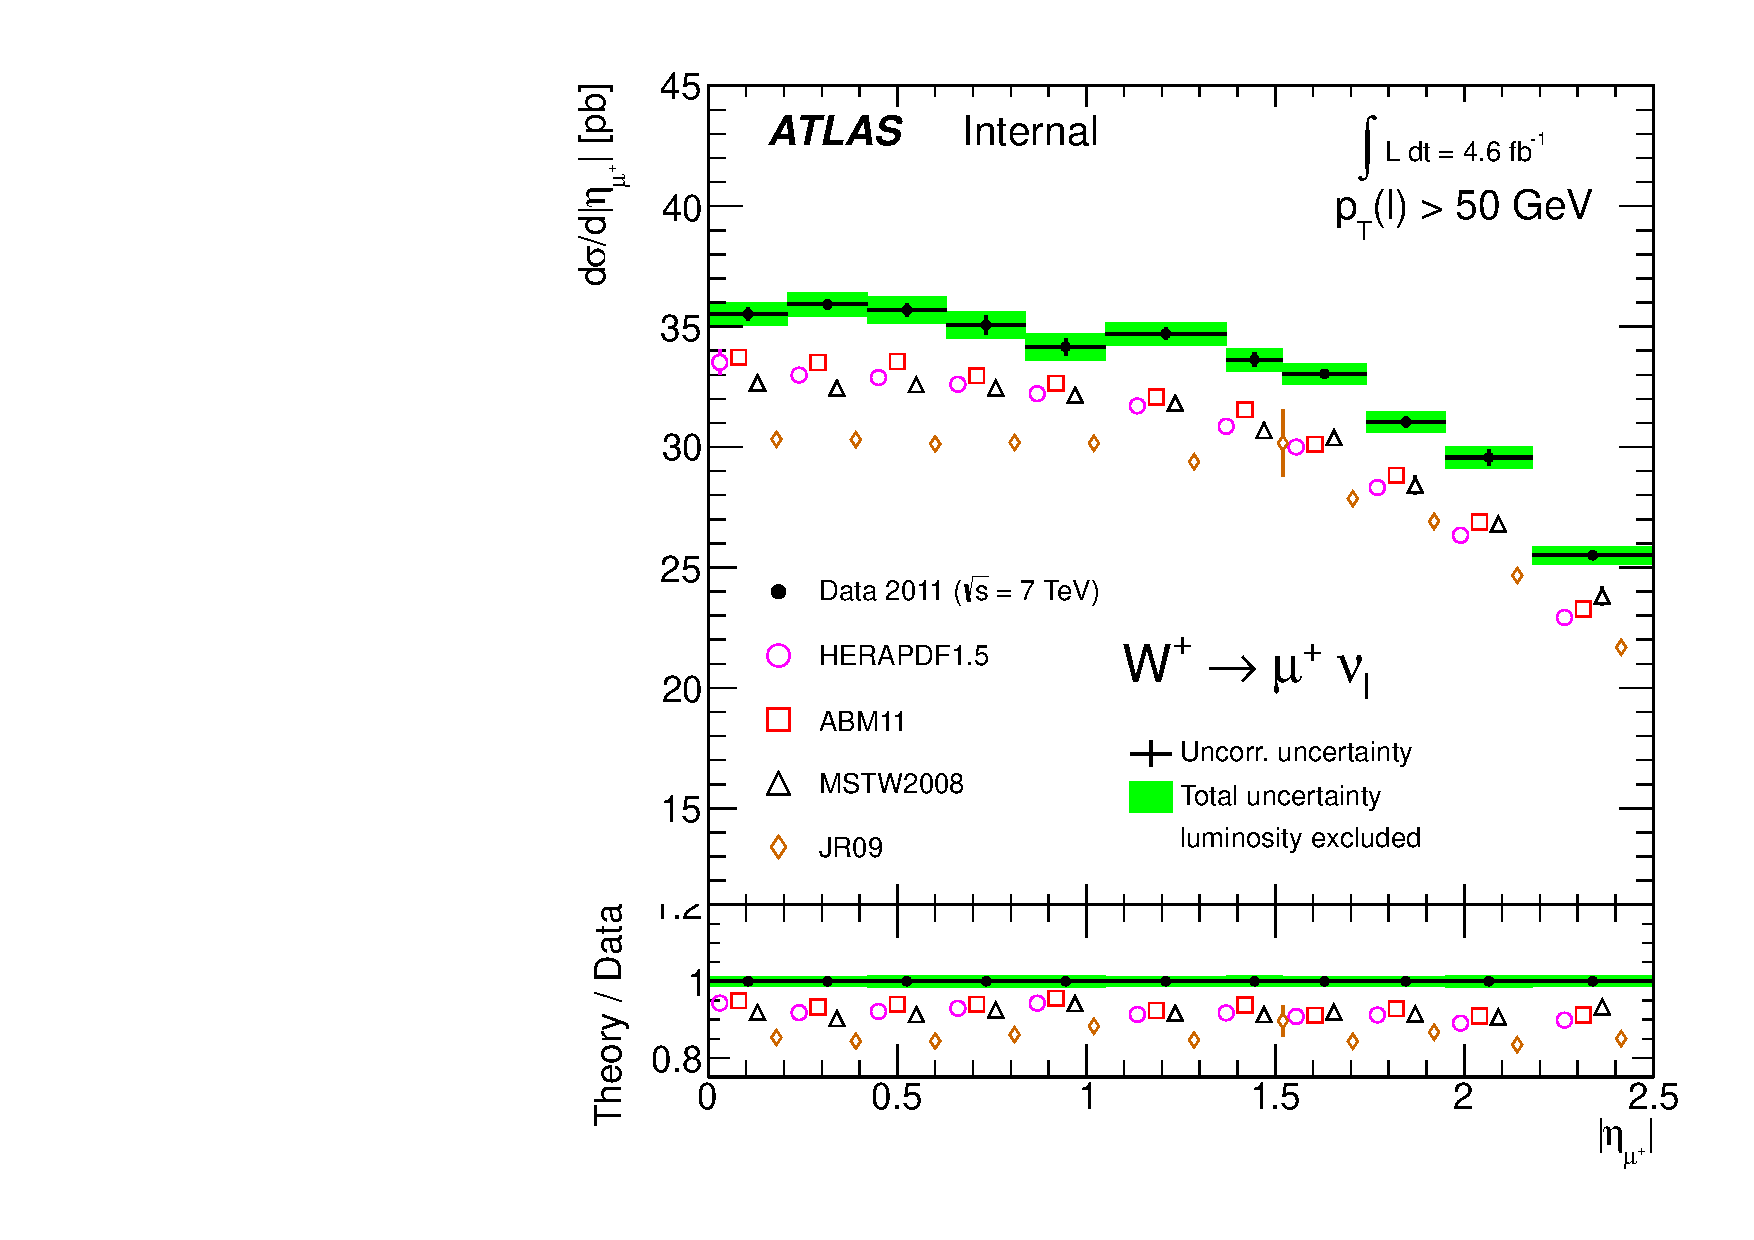
\includegraphics[width=0.55\textwidth]{res/fig/WPetaPt50_NNLO_combined}
       } 
 \caption{ The double-differential cross-section measurement for \Wplusmunu\ in $p_T$ slices: \ptFive\ and \ptSix. NNLO QCD predictions using various PDF sets (open symbols) are compared to the data (full points). For technical reasons, the uncertainty on predictions excludes the uncertainty from the PDF error envelope. }
 \label{fig:Comb:NNLO:W2dPOS_3}
 \end{center}
\end{figure}

%% \begin{figure}[phtb]
%%   \begin{center}
%%         \subfigure[\ptOne]{%
%% 	  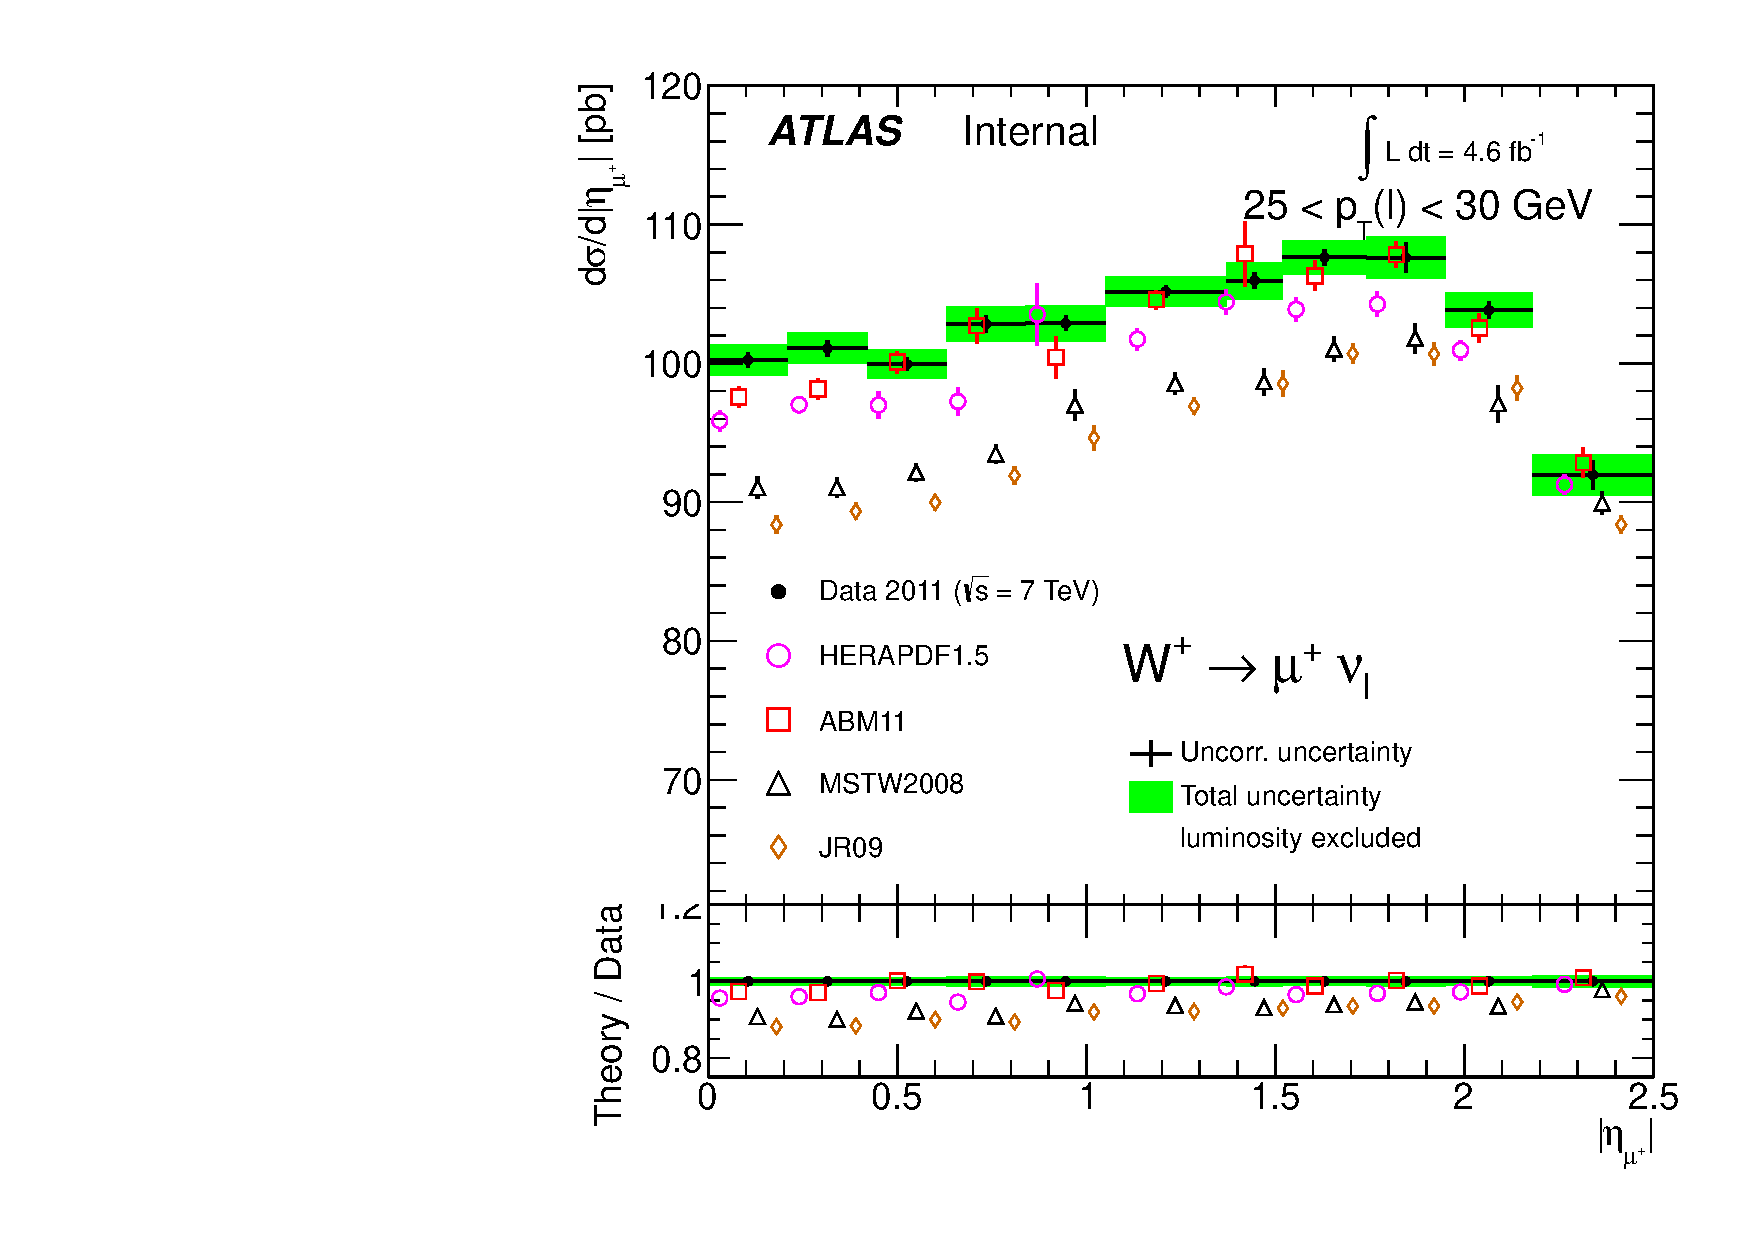
\includegraphics[width=0.36\textwidth]{res/fig/WPetaPt25_30_NNLO_combined}
%%         }
%%        \subfigure[\ptTwo]{%
%% 	  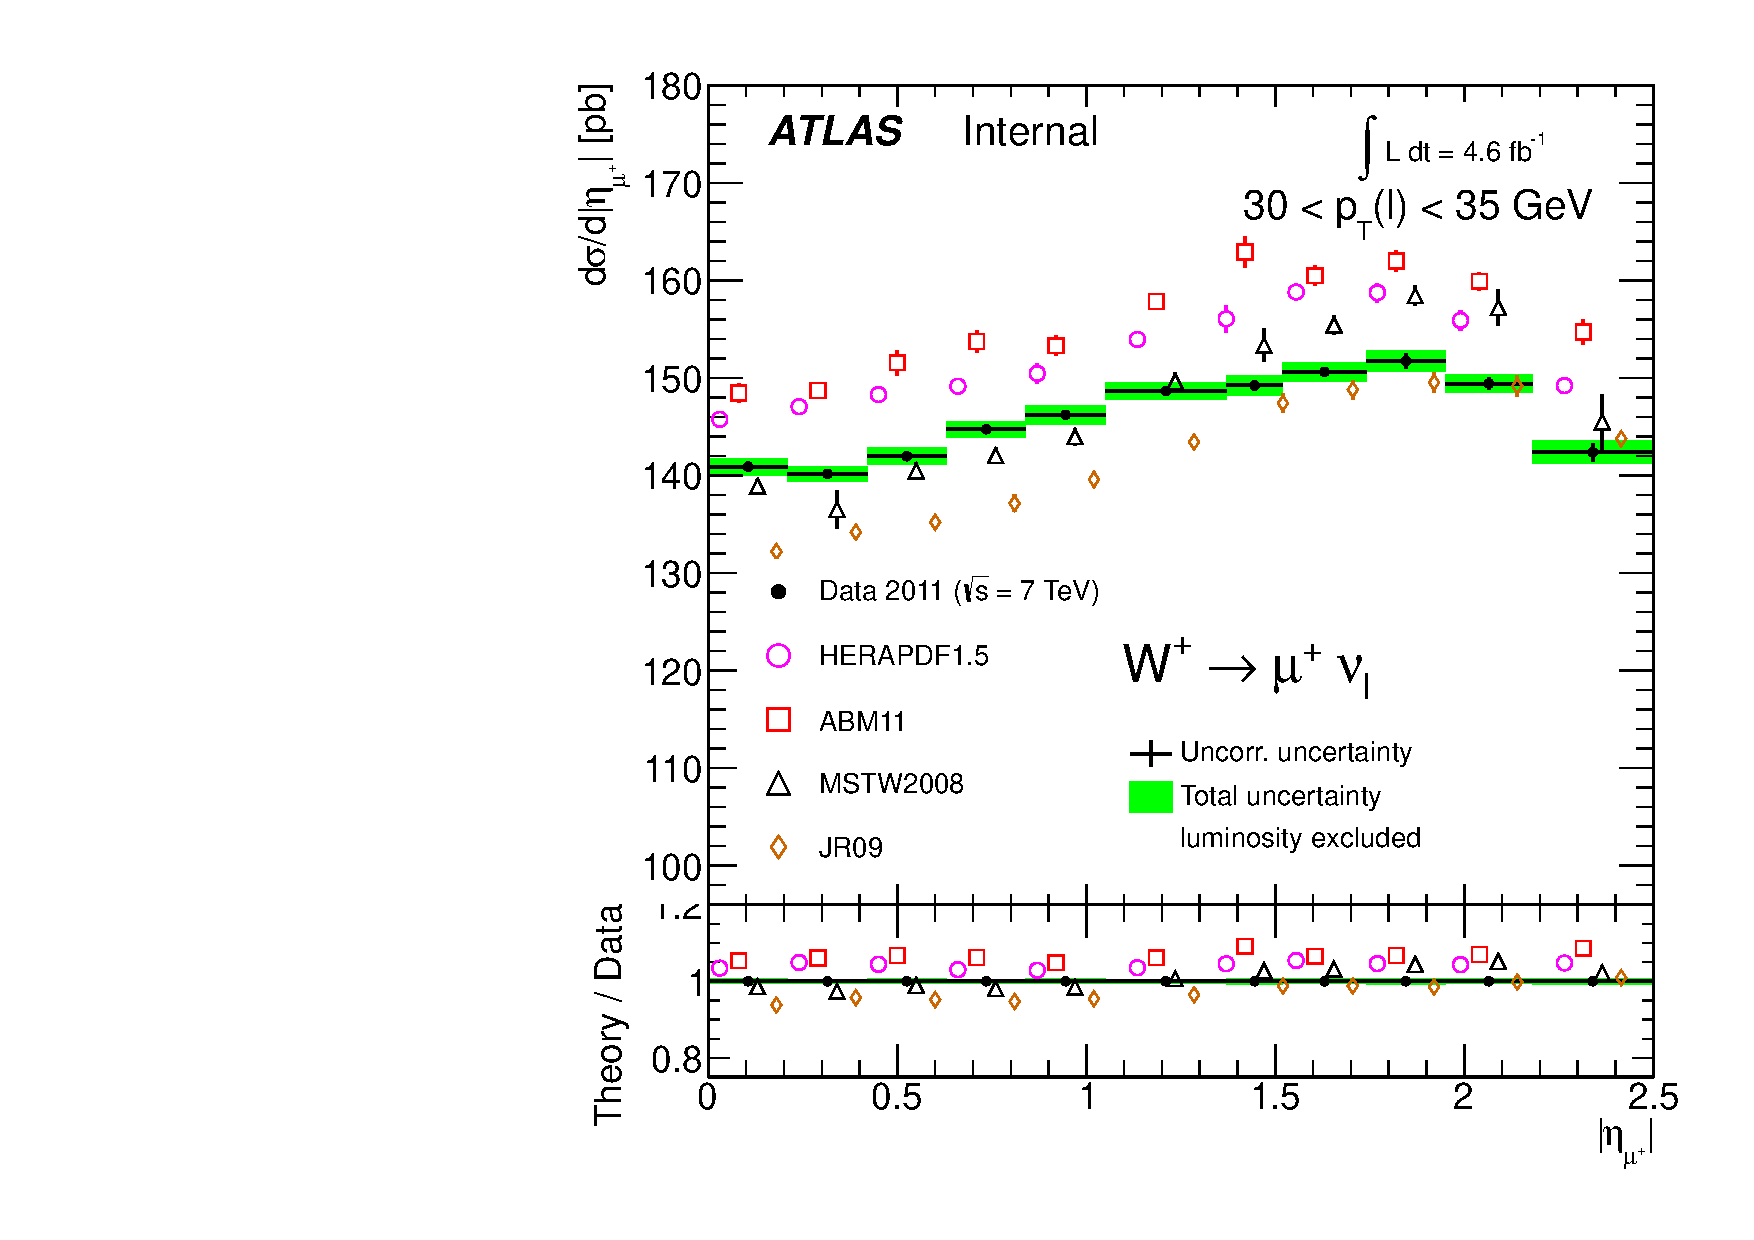
\includegraphics[width=0.36\textwidth]{res/fig/WPetaPt30_35_NNLO_combined}
%%         } \\
%%        \subfigure[\ptThree]{%
%% 	  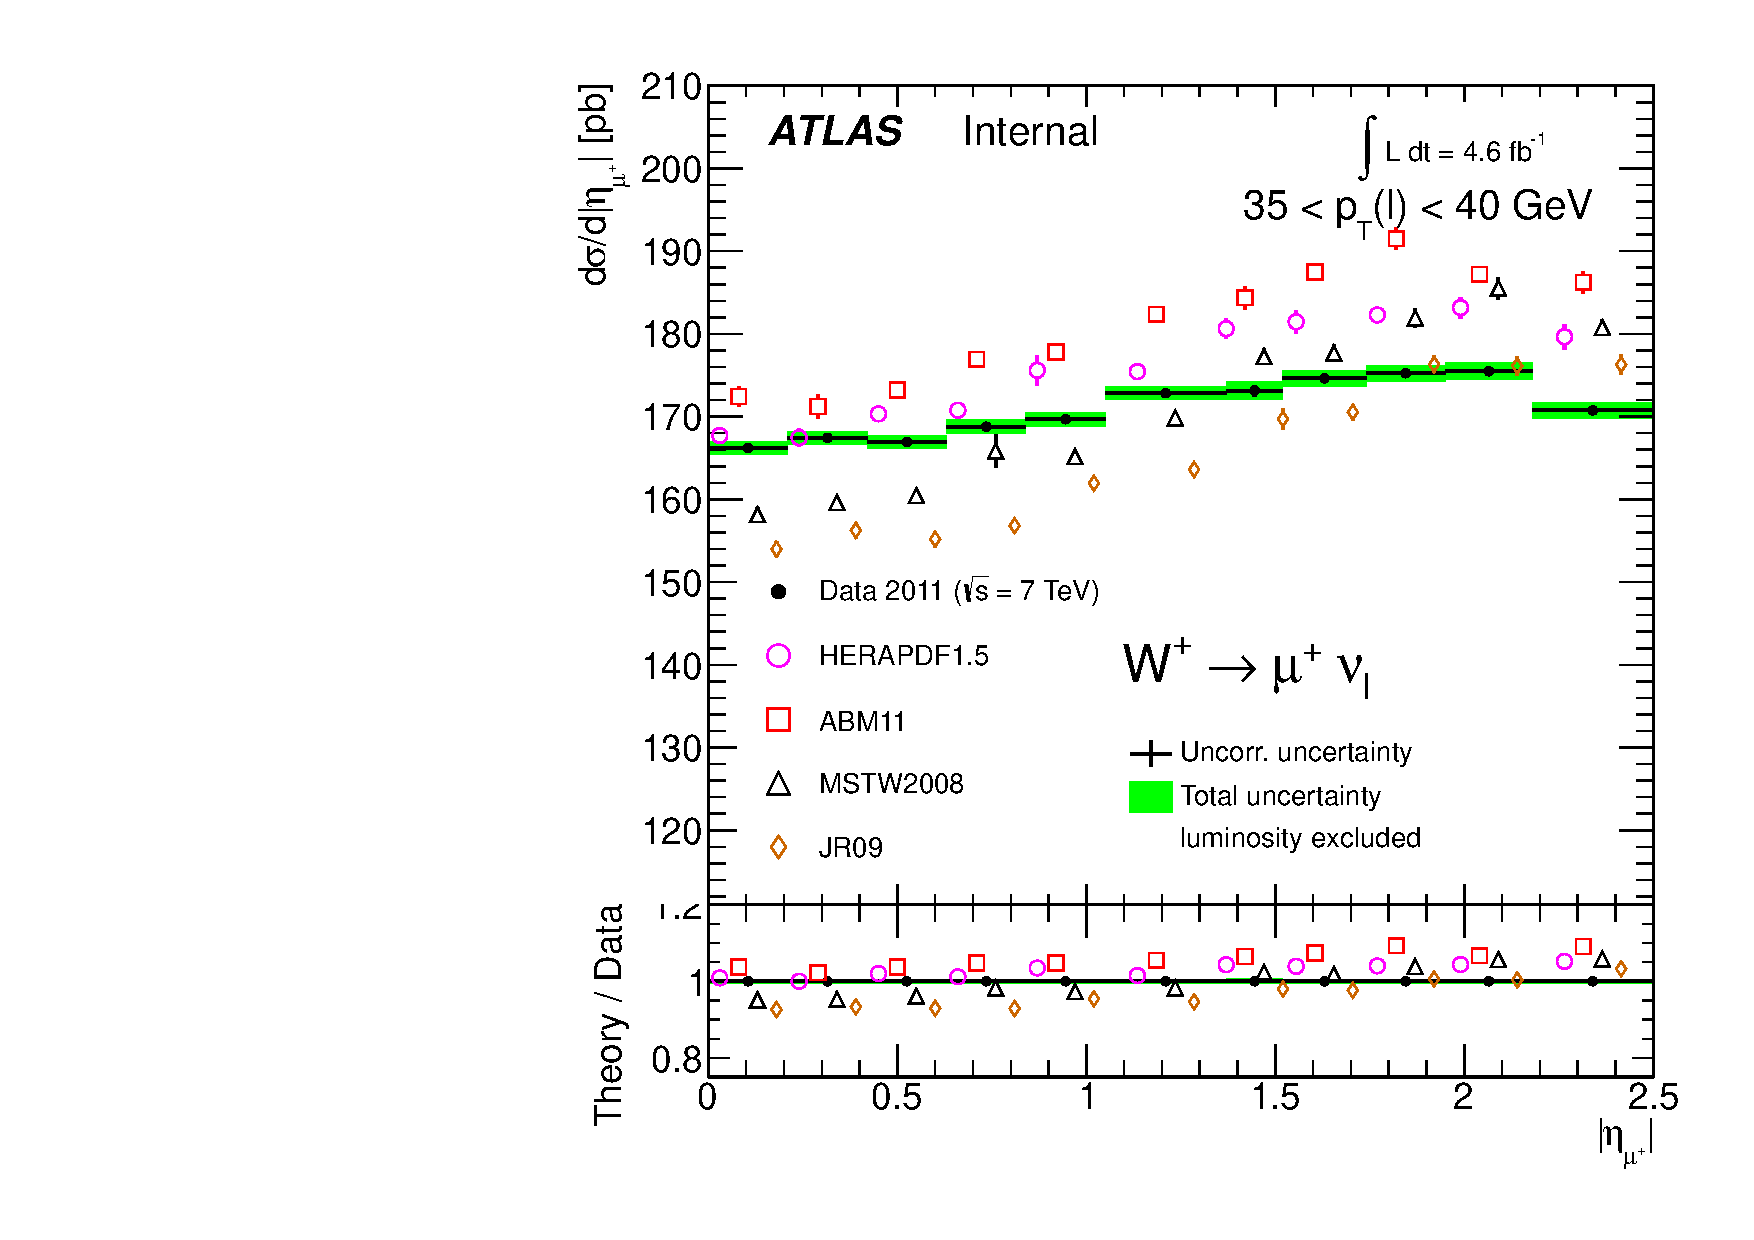
\includegraphics[width=0.36\textwidth]{res/fig/WPetaPt35_40_NNLO_combined}
%%         }
%%        \subfigure[\ptFour]{%
%% 	  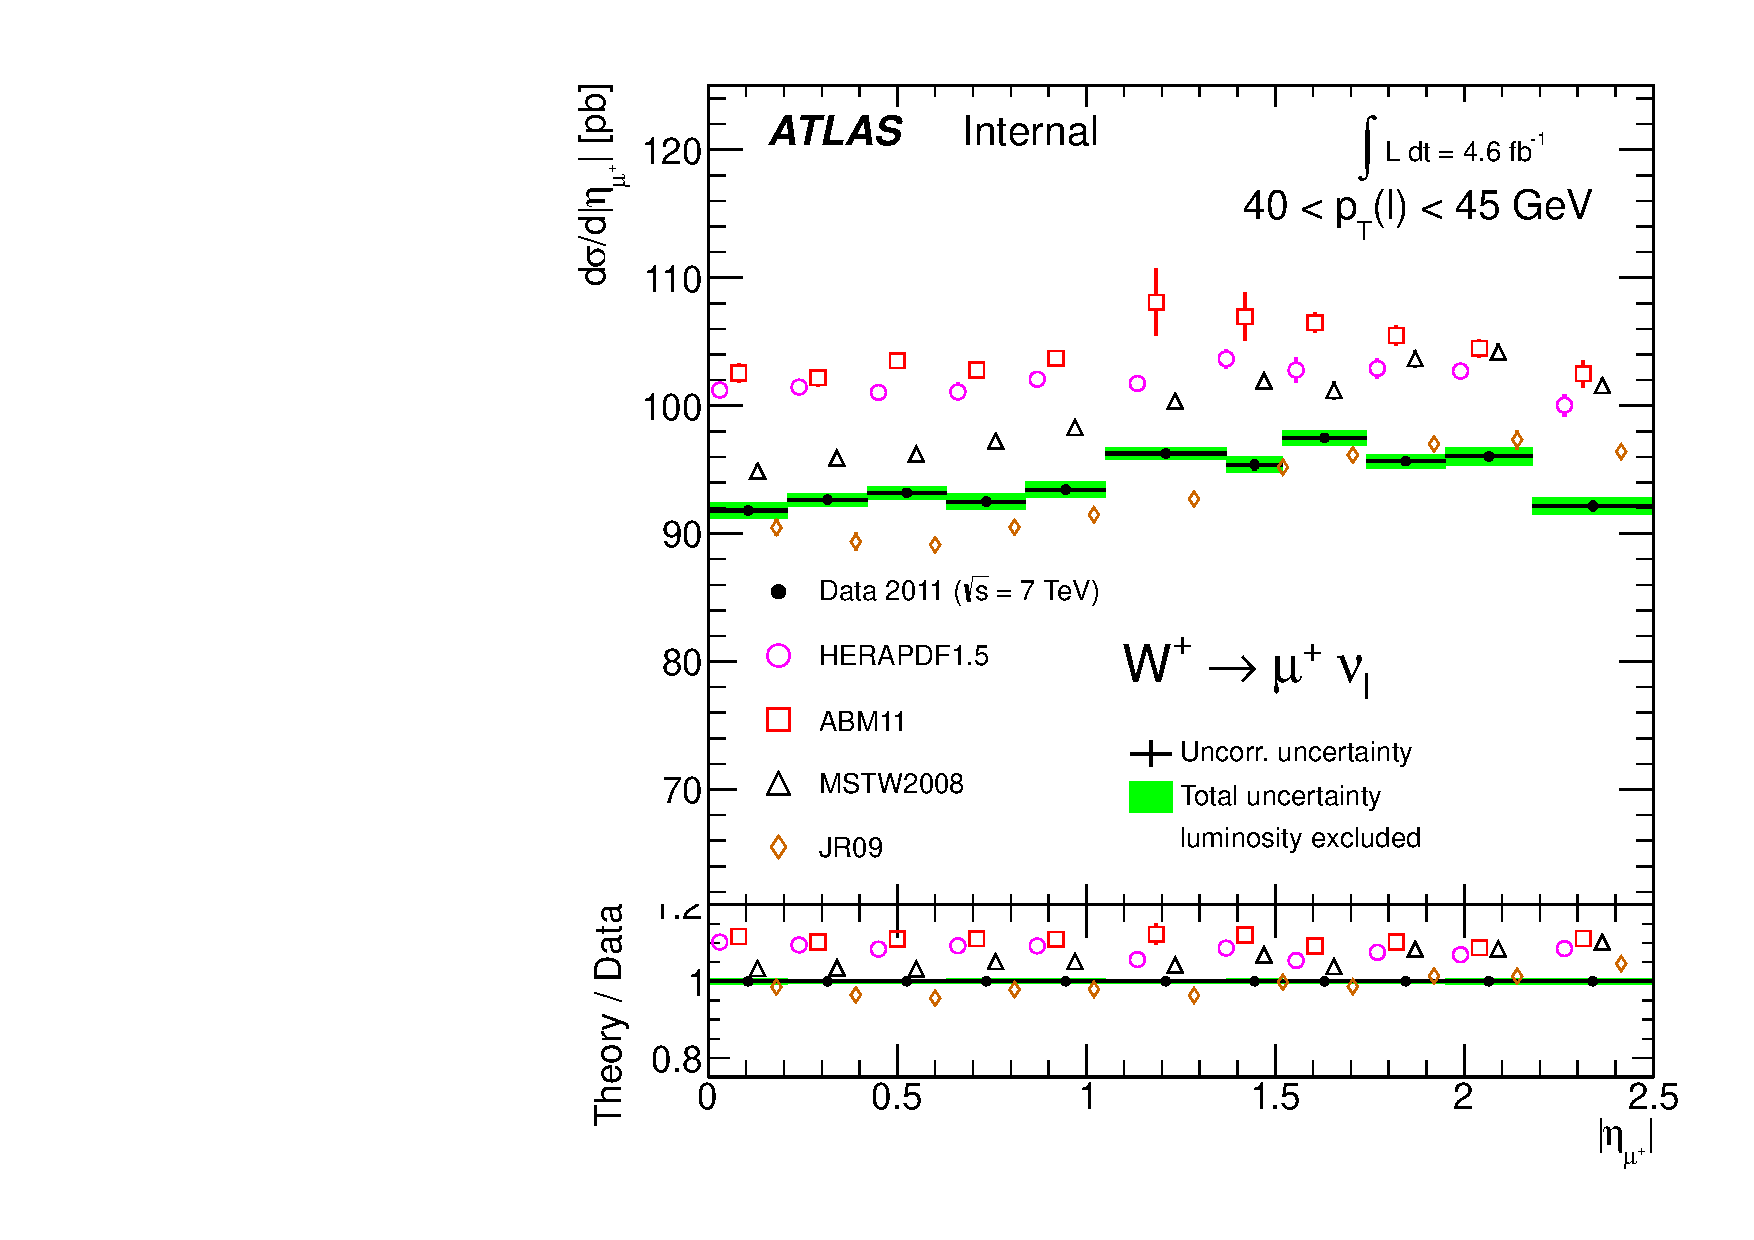
\includegraphics[width=0.36\textwidth]{res/fig/WPetaPt40_45_NNLO_combined}
%%         } \\
%%        \subfigure[\ptFive]{%
%% 	  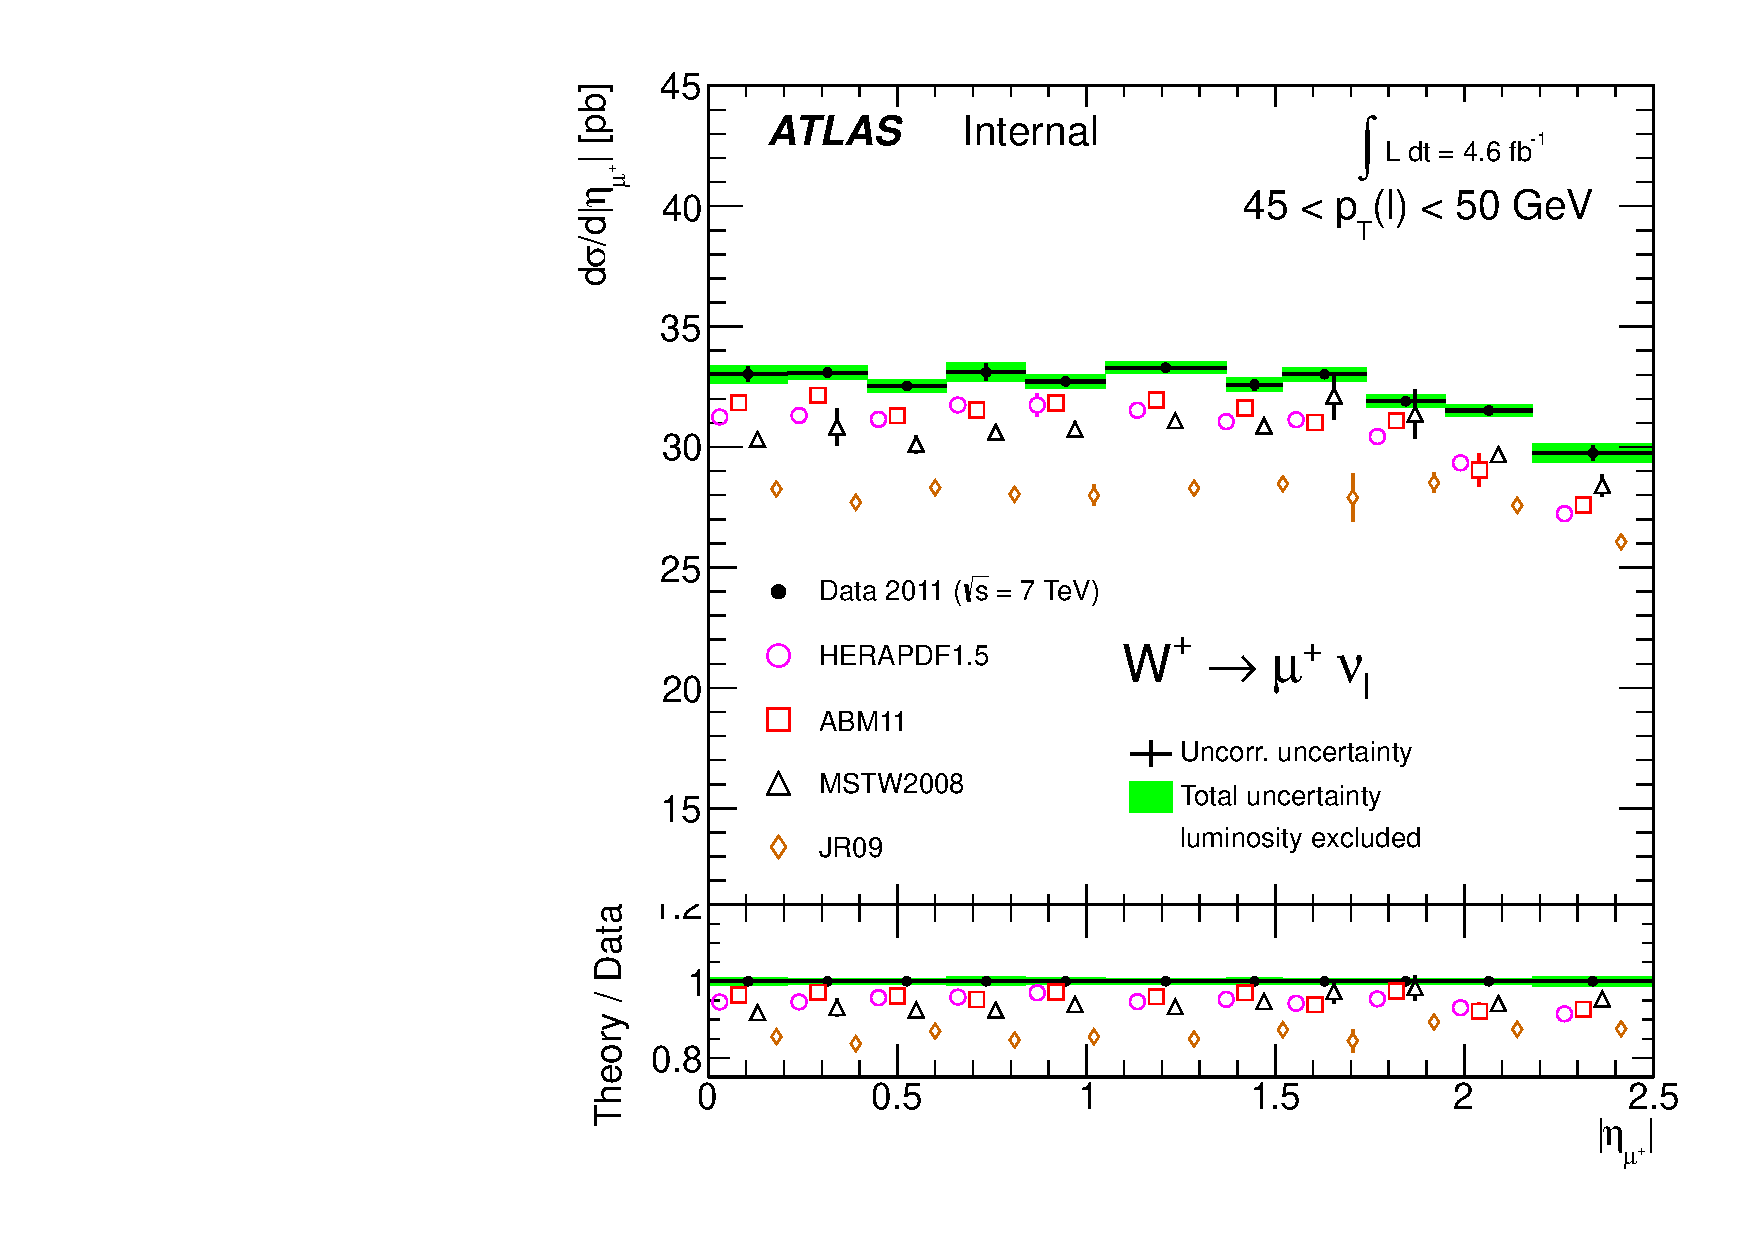
\includegraphics[width=0.36\textwidth]{res/fig/WPetaPt45_50_NNLO_combined}
%%         }
%%        \subfigure[\ptSix]{%
%% 	  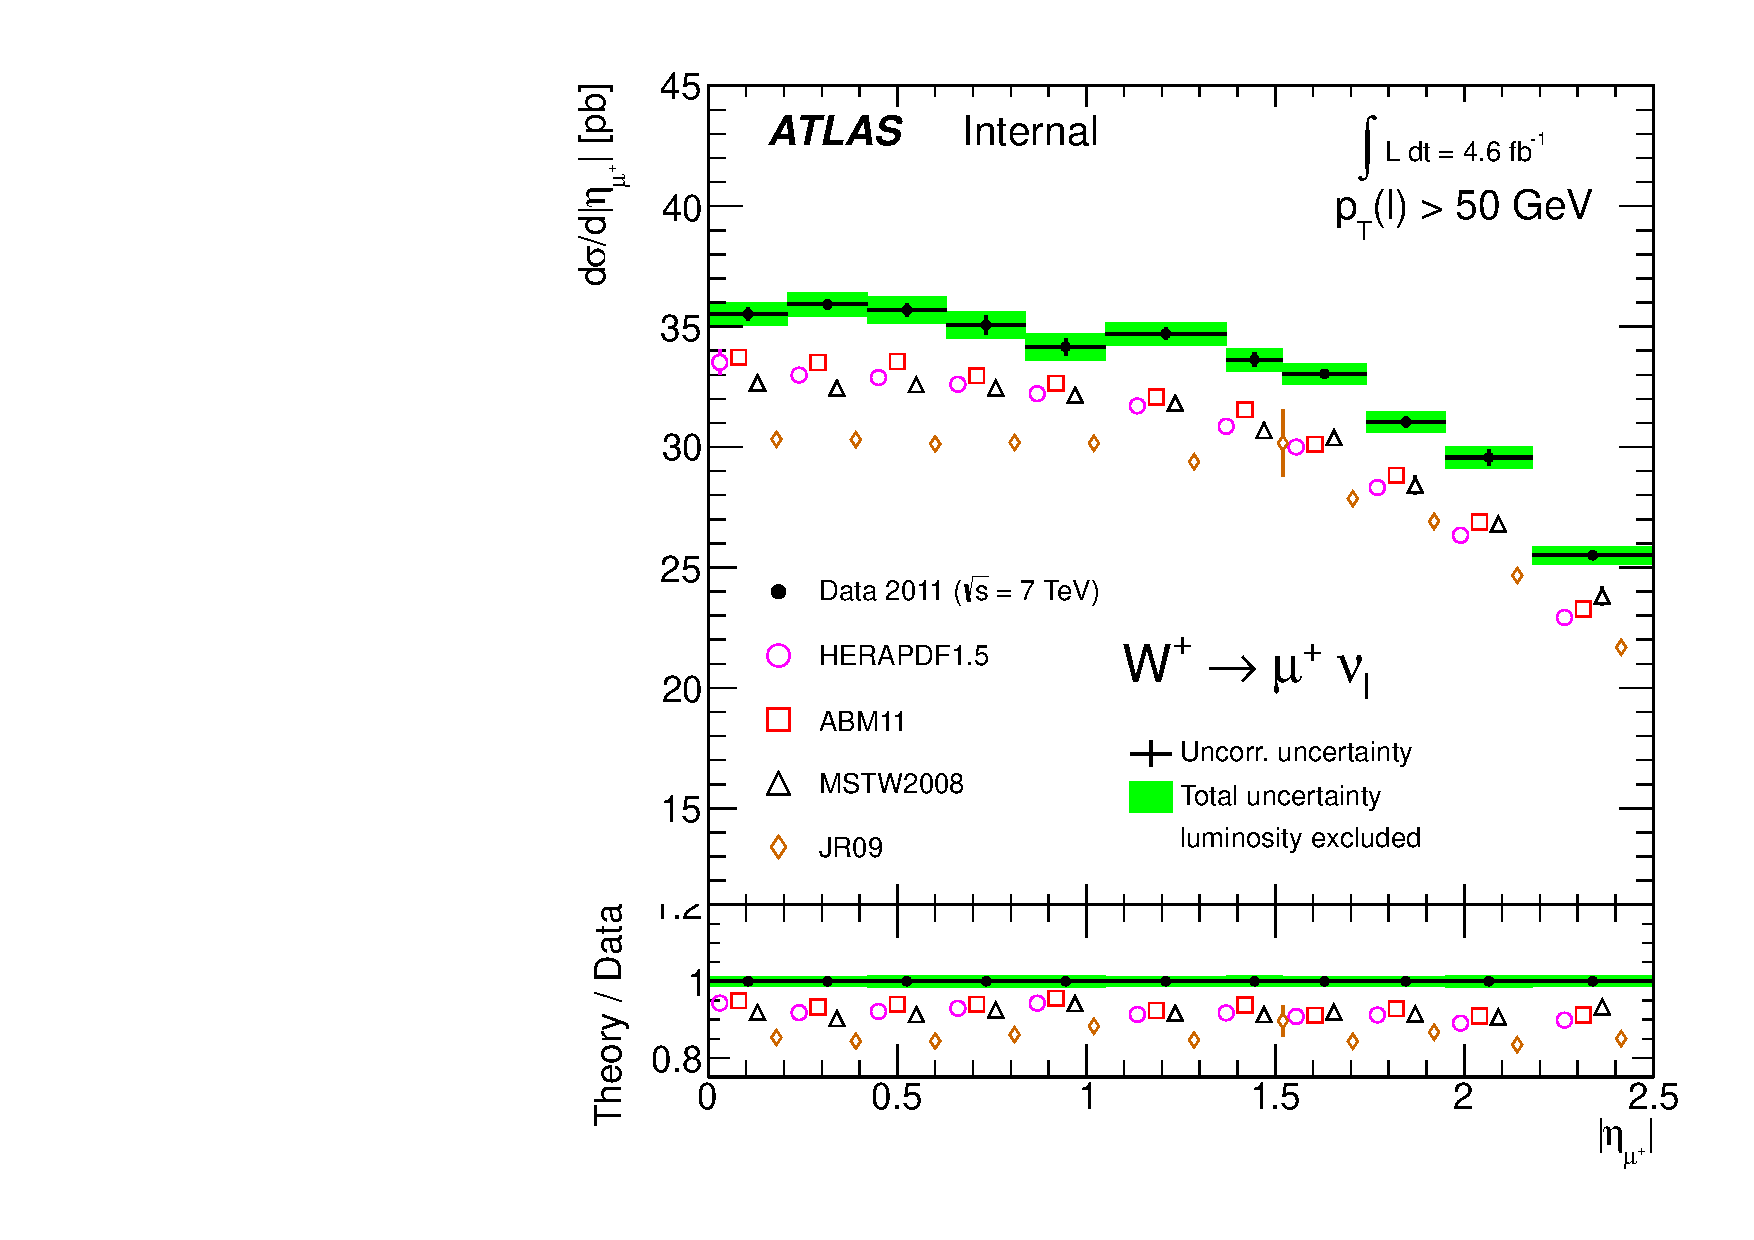
\includegraphics[width=0.36\textwidth]{res/fig/WPetaPt50_NNLO_combined}
%%        } 
%%  \caption{ The double-differential cross-section measurement for \Wplusmunu\ in $p_T$ slices. NNLO QCD predictions using various PDF sets (open symbols) are compared to the data (full points). For technical reasons, the uncertainty on predictions excludes the uncertainty from the PDF error envelope. }
%%  \label{fig:Comb:NNLO:W2dPOS}
%%  \end{center}
%% \end{figure}

\clearpage
\section{ PDF Fit Analysis }
Measurement of differential cross-sections can potentially provide new constraints on Parton Distribution Functions (PDFs), as explained in Sec.~\ref{sec:theory:pdfrap}. The efforts to integrate the results of this measurement into global PDF fits are in progress. Some preliminary results are presented below.

\subsection{ Combination }
In order to maximize the power of differential cross-sections to constrain PDFs, measurements in the \Wmn, \Wen, \Zmm, and \Zee\ channels are first combined taking into account the correlations of systematics across bins and measurement channels (see Tab.~\ref{tab:SystCorr}). The combination is performed using a standard Fortran package first developed for the combination of deep inelastic scattering data at HERA~\cite{glazov}.

At this time, only single-differential measurements can be used in the PDF analysis machinery. The $\chi^2$ of the combination divided by the number of degrees of freedom is $54.68/53$, suggesting that the measurements in all channels are compatible within their uncertainties.

\begin{table}[htbp]   
\small
  \begin{center}
    \begin{tabular}{lccccc}
      \hline
      \hline
      & \multicolumn{5}{c}{Channel} \\
      Uncertainty Source & \Wen\ & \Zee\ & \Zee\ (CF) & \Wmn\ & \Zmm\  \\
      \hline
      \input{tables/systematic_correlations.tex}
      \hline
      \hline
    \end{tabular}
  \end{center}
    \caption{Summary of the correlations for the uncertainties. Each number represents a nuisance
parameter. Cells with a shared nuisance parameter are treated as correlated, whereas cells containing
$u$ are treated as uncorrelated. $uN$ represents an uncertainty which is uncorrelated bin-to-bin, but
correlated across cells with the same $N$. The highlighted entries illustrate each type of cross-channel correlation. }
    \label{tab:SystCorr}
\end{table}

\subsection{ PDF sensitivity }

The PDF fits are performed using the HERAFitter framework~\cite{HERAFitter,Aaron:2009aa,Aaron:2009kv}, which relies on QCDNUM~\cite{Botje:2010ay} for PDF evolution and MINUIT~\cite{James:1975dr} for fit minimization. Convolution of hard scatter cross-sections with PDF weights is performed with the APPLGRID technique~\cite{Carli:2010rw}, while theoretical calculations are done using the MCFM program~\cite{Campbell:2010ff}.

Deep inelastic scattering data from HERA I is used to define a baseline PDF family, which is then augmented with the combined ATLAS data. The fit takes into account all experimental uncertainties in order to properly account for correlations between $|\eta|$ bins.

Fig.~\ref{fig:QCDFit:Wpm} shows the pulls\footnote{The pulls are defined as differences between the measured and predicted values in each bin, divided by the total bin error.} in the fits to \Wpm\ cross-sections vs $|\eta|$. The large luminosity uncertainty is mitigated by allowing the normalization to float, resulting in an overall shift that is consistent between $W^+$ and $W^-$. The data are consistent with the fitted PDF: the sum of the pulls across all 11 measured $|\eta|$ bins produces an overall $\chi^{2}/DOF \approx 13/11$, corresponding to a $\chi^{2}$ probability of 29\%.

\begin{figure}
  \begin{center}
    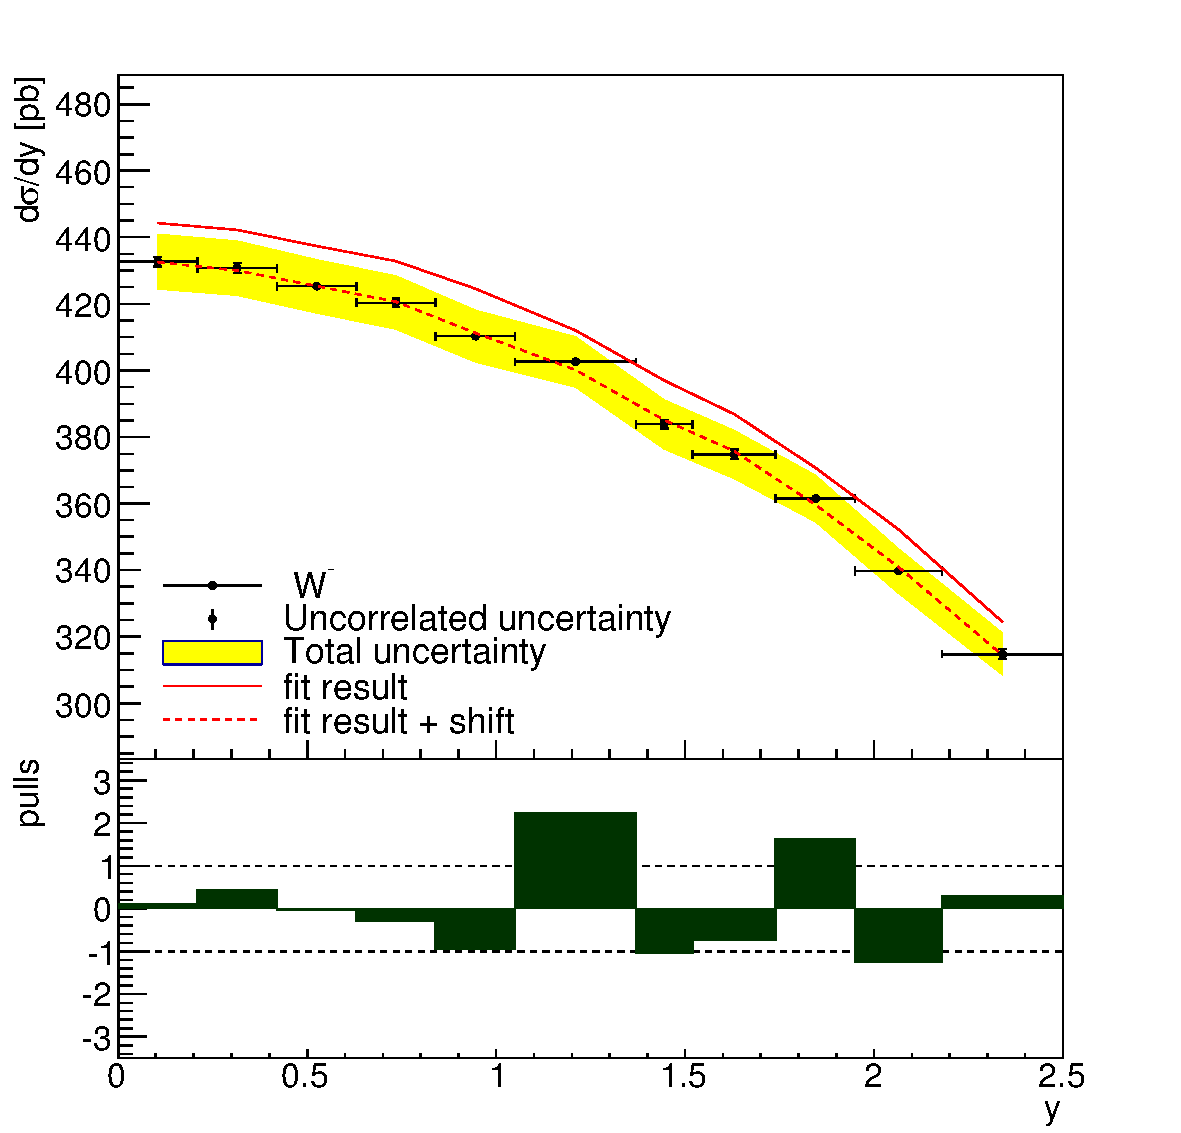
\includegraphics[width=0.60\textwidth]{res/fig/pulls_104}
    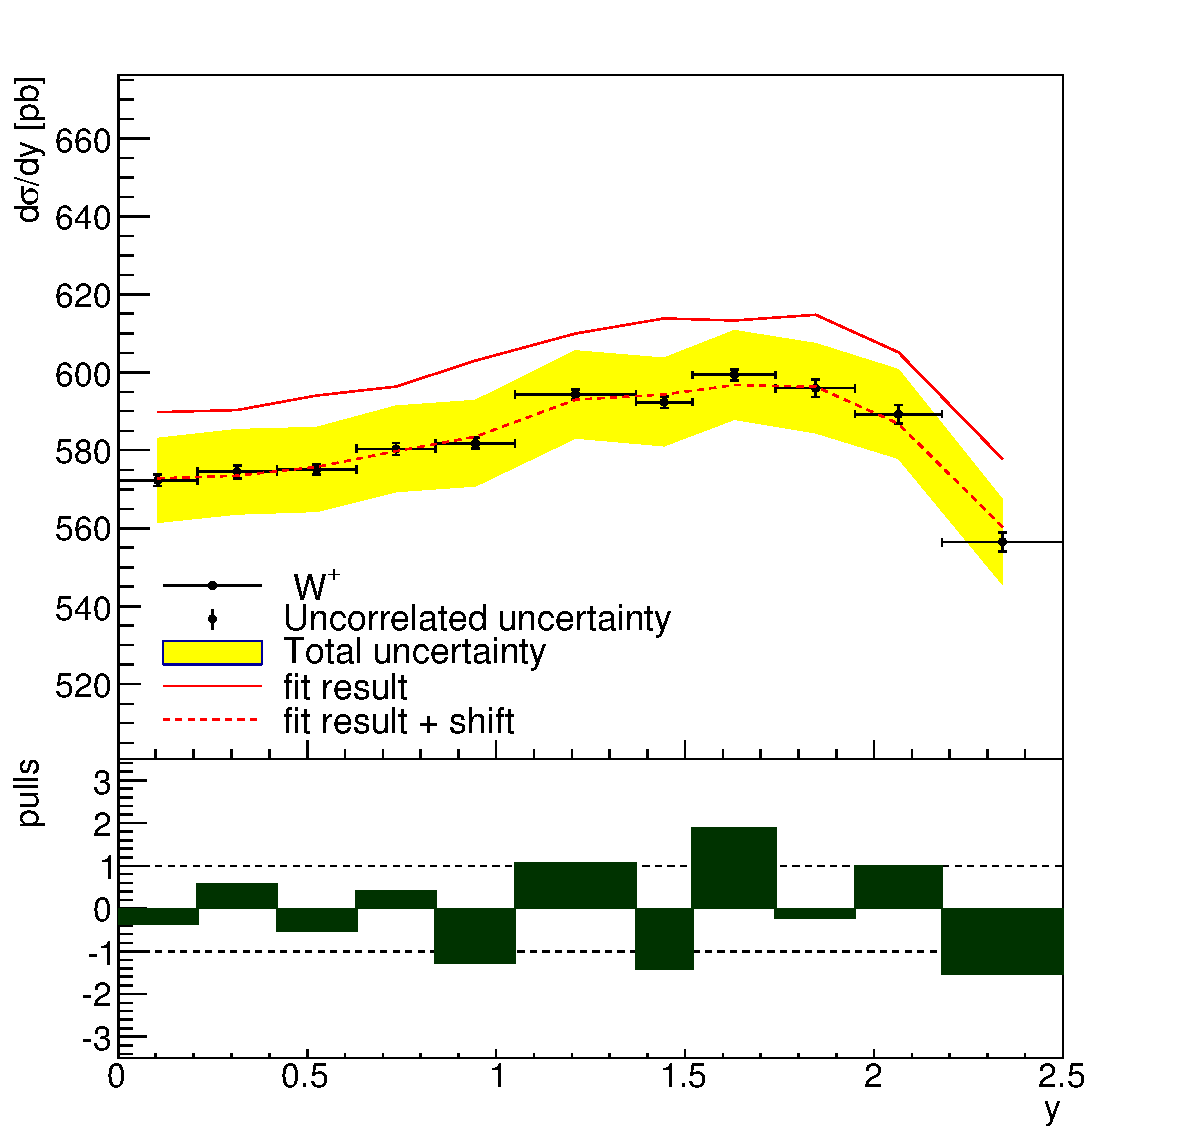
\includegraphics[width=0.60\textwidth]{res/fig/pulls_105}
  \end{center}
  \caption{ The differential $d\sigma/d|\eta_{\ell^{-}}|$ (top) and $d\sigma/d|\eta_{\ell^{+}}|$ (bottom) cross-section measurement for $W \rightarrow \ell\nu$. The lower box shows the normalized data-theory pulls after the shifts of the correlated uncertainties (e.g., luminosity) are applied. }
  \label{fig:QCDFit:Wpm}
\end{figure}

Fig.~\ref{fig:ZW_PDF_sensitivity} illustrates the combined effect of 2011 \Wpmln\ and \Zll\ measurements on the parton distribution functions. Good sensitivity is obtained on the valence down quark PDF (mostly driven by \Wpmln) and the strange quark sea PDF (mostly driven by \Zll), while only a moderate impact is seen on the valence up quark.

\begin{figure}
\begin{center}
\includegraphics[width=0.60\textwidth]{QCD/figures/ZWu_dval_pdf_hess.pdf} \\
\includegraphics[width=0.60\textwidth]{QCD/figures/ZWu_uval_pdf_hess.pdf} \\
\includegraphics[width=0.60\textwidth]{QCD/figures/ZWu_s_pdf_hess.pdf}
\caption{Sensitivity of \Wpmln\ and \Zll\ 2011 measurements to the $xd_{val}(x)$ (top), $xu_{val}(x)$ (middle), and $xs$ (bottom). }
\label{fig:ZW_PDF_sensitivity}
\end{center}
\end{figure}

\clearpage
\section{ Lepton Universality }

The lepton universality principle states that the coupling of leptons to gauge bosons is flavor-independent. The universality can be probed directly by comparing the integrated \Wmn\ and \Wen\ cross-sections, and separately \Zmm\ and \Zee\ cross-sections. Fig.~\ref{Fig:lUniFid} illustrates the ratios of these cross-sections and compares them with the PDG world average. The new data confirms the lepton universality and, in the case of W cross-sections, provides better precision than the current world average.

\begin{figure}
  \begin{center}
    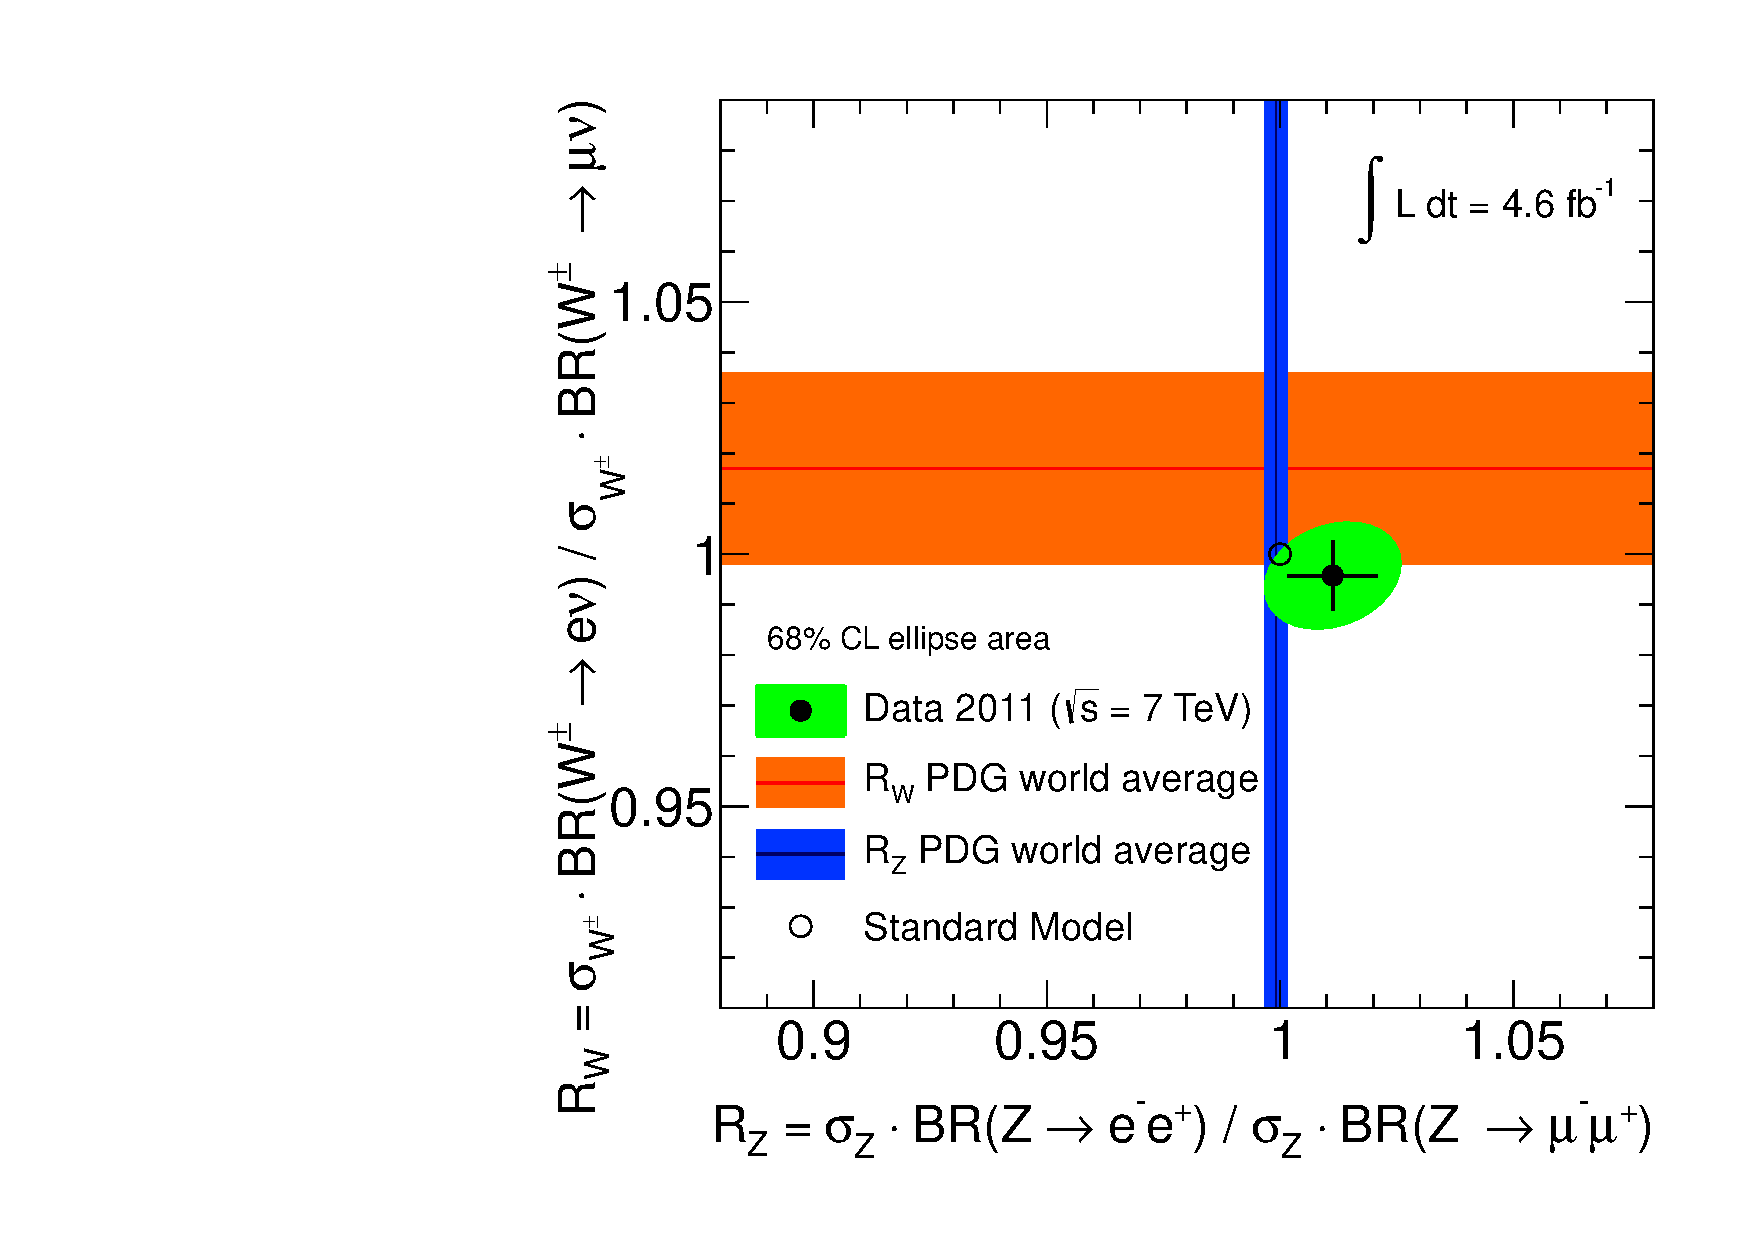
\includegraphics[width=0.75\textwidth]{res/fig/ZWluni_ellipse}
  \end{center}
\caption{The measurement of the electron-to-muon cross-section ratios for the $W$ and $Z$ production.
The shaded bands represent the world average of the ratios of electron and muon branching fractions
for $W$ and $Z$. The green shaded ellipse represents the $68\%$ CL for the correlated measurement of $R_{W}$ and $R_{Z}$}
\label{Fig:lUniFid}
\end{figure}
